
% this is for R kableExtra table output `striped'
\PassOptionsToPackage{table}{xcolor}

\PassOptionsToPackage{unicode}{hyperref}
\PassOptionsToPackage{naturalnames}{hyperref}

\documentclass[oneside,12pt,letterpaper]{article}

%%%%%%%%%%%%%%%%%%%%%%%%%%%%%%%%%%%%%%%%%%%%%%%%%%%%%%%%%%%%%
% title and authors
%%%%%%%%%%%%%%%%%%%%%%%%%%%%%%%%%%%%%%%%%%%%%%%%%%%%%%%%%%%%%
\usepackage{authblk} % provide \affil

%%%%%%%%%%%%%%%%%%%%%%%%%%%%%%%%%%%%%%%%%%%%%%%%%%%%%%%%%%%%%
% mathematics
%%%%%%%%%%%%%%%%%%%%%%%%%%%%%%%%%%%%%%%%%%%%%%%%%%%%%%%%%%%%%
% some mathematics packages
% avoid mathabx package at all cost
\usepackage{amsmath,amssymb,bm,bbold}
\usepackage{amsfonts,amsthm,mathrsfs,mathtools}
\usepackage{stmaryrd}
\SetSymbolFont{stmry}{bold}{U}{stmry}{m}{n}
\usepackage{upgreek}
% \usepackage{physics}
\usepackage{stmaryrd}
\usepackage{econometrics}
\usepackage{breqn}
% \breqnsetup{breakdepth={1}}

%%%%%%%%%%%%%%%%%%%%%%%%%%%%%%%%%%%%%%%%%%%%%%%%%%%%%%%%%%%%%
% graphics and others
%%%%%%%%%%%%%%%%%%%%%%%%%%%%%%%%%%%%%%%%%%%%%%%%%%%%%%%%%%%%%
\usepackage{tikz}
\usetikzlibrary{positioning}
\usepackage{xr-hyper}
\usepackage{pdfpages}
\usepackage{pgf,interval}

%%%%%%%%%%%%%%%%%%%%%%%%%%%%%%%%%%%%%%%%%%%%%%%%%%%%%%%%%%%%%
% table and figures
%%%%%%%%%%%%%%%%%%%%%%%%%%%%%%%%%%%%%%%%%%%%%%%%%%%%%%%%%%%%%
\usepackage{float}
\usepackage{booktabs, array, longtable, ragged2e, pdflscape}
\usepackage{subcaption}

%%%%%%%%%%%%%%%%%%%%%%%%%%%%%%%%%%%%%%%%%%%%%%%%%%%%%%%%%%%%%
% appendix, index, and toc
%%%%%%%%%%%%%%%%%%%%%%%%%%%%%%%%%%%%%%%%%%%%%%%%%%%%%%%%%%%%%
\usepackage{hyperref}
\hypersetup{
  colorlinks = false,
  urlbordercolor = {blue},
  linkbordercolor = {red},
  citebordercolor = {green}
}
\usepackage[page,toc,titletoc,title]{appendix}
\usepackage{makeidx}
\usepackage[nottoc,numbib]{tocbibind}
\hypersetup{bookmarksopen=true}


%%%%%%%%%%%%%%%%%%%%%%%%%%%%%%%%%%%%%%%%%%%%%%%%%%%%%%%%%%%%%
% cross-reference
%%%%%%%%%%%%%%%%%%%%%%%%%%%%%%%%%%%%%%%%%%%%%%%%%%%%%%%%%%%%%
\usepackage{cleveref}
\renewcommand{\cref}{\Cref}
\renewcommand{\crefrange}{\Crefrange}


%%%%%%%%%%%%%%%%%%%%%%%%%%%%%%%%%%%%%%%%%%%%%%%%%%%%%%%%%%%%%
% algorithm
%%%%%%%%%%%%%%%%%%%%%%%%%%%%%%%%%%%%%%%%%%%%%%%%%%%%%%%%%%%%%
\usepackage{algorithm}
% \usepackage{algorithmic}
\usepackage{algpseudocode}
% \usepackage{algpseudocodex}
% \floatname{algorithm}{Procedure}
\algnewcommand\algorithmicinput{\textbf{Initialize:}}
\algnewcommand\Initialize{\item[\algorithmicinput]}
\renewcommand{\algorithmicrequire}{\textbf{Input:}}
\renewcommand{\algorithmicensure}{\textbf{Output:}}

%%%%%%%%%%%%%%%%%%%%%%%%%%%%%%%%%%%%%%%%%%%%%%%%%%%%%%%%%%%%%
% load some fonts
%%%%%%%%%%%%%%%%%%%%%%%%%%%%%%%%%%%%%%%%%%%%%%%%%%%%%%%%%%%%%
% remove the font size not available warning (but change the font)
% \usepackage{lmodern,anyfontsize,libertinus}

%%%%%%%%%%%%%%%%%%%%%%%%%%%%%%%%%%%%%%%%%%%%%%%%%%%%%%%%%%%%%
% bibliography
%%%%%%%%%%%%%%%%%%%%%%%%%%%%%%%%%%%%%%%%%%%%%%%%%%%%%%%%%%%%%
% OLD bibtex KEEP FOR REFERENCE
% \bibliographystyle{apalike}
% \usepackage{doi,natbib}
% \bibliography{{../Metalearner.bib}} % add at the end


% default to newer biblatex
\usepackage[american]{babel}
\usepackage{csquotes}
\usepackage[
  style=authoryear,maxnames=3,natbib=true,uniquename=false,
  isbn=false,url=false,eprint=false,date=year,dashed=false
]{biblatex}
\bibliography{wig-r.bib}
\DefineBibliographyStrings{english}{bibliography = {References}}


% change the font of the bibliography
% \renewcommand*{\bibfont}{\normalfont\scriptsize}

%%%%%%%%%%%%%%%%%%%%%%%%%%%%%%%%%%%%%%%%%%%%%%%%%%%%%%%%%%%%%
% other packages
%%%%%%%%%%%%%%%%%%%%%%%%%%%%%%%%%%%%%%%%%%%%%%%%%%%%%%%%%%%%%
% \usepackage{filecontents}
\usepackage{xcolor}
\usepackage{cancel} % strikethrough line
\usepackage[left=2.5cm, right=2.5cm, top=3cm]{geometry}
\usepackage{indentfirst}
\usepackage{fancyhdr}
\setlength{\headheight}{27.5pt}
\pagestyle{fancy}

%%%%%%%%%%%%%%%%%%%%%%%%
\newcommand\deq{\stackrel{\mathclap{\normalfont\mbox{d}}}{=}}

%%%%%%%%%%%%%%%%%%%%%%%%%%%%%%%%%%%%%%%%%%%%%%%%%%%%%%%%%%%%%%
% underbar problem
%%%%%%%%%%%%%%%%%%%%%%%%%%%%%%%%%%%%%%%%%%%%%%%%%%%%%%%%%%%%%%
% \usepackage{accents} % don't work with econometrics
% \newcommand\munderbar[1]{\underaccent{\bar}{#1}} 
\newcommand{\ubar}[1]{\text{\b{$#1$}}} % without using accents package
% \newcommand\expe{\mathop{{}\mathbb{E}}}

%%%%%%%%%%%%%%%%%%%%%%%%%%%%%%%%%%%%%%%%%%%%%%%%%%%%%%%%%%%%%%
% fix the underbrace problem
% link: https://tex.stackexchange.com/questions/457134
% mathtools redefines overbrace and underbrace from mathabx
%%%%%%%%%%%%%%%%%%%%%%%%%%%%%%%%%%%%%%%%%%%%%%%%%%%%%%%%%%%%%%
\let\underbrace\LaTeXunderbrace%
\let\overbrace\LaTeXoverbrace%

% define \circled{} macro
\usepackage{enumitem}
\newcommand*\circled[1]{%
  \tikz[baseline=(char.base)]{\node[shape=circle,draw,inner sep=1.5pt] (char) {#1};}
}

% define \yes and \no for checkmarks
\usepackage{pifont}% http://ctan.org/pkg/pifont
\newcommand{\yes}{\ding{51}}%
\newcommand{\no}{\ding{55}}%

% % define interior macro
\newcommand{\interior}[1]{%
  {\kern0pt#1}^{\mathrm{o}}%
}
\newcommand{\intr}[1]{\interior{#1}}

%% define diag function
% \newcommand{\diag}{\text(diag)}

% % define argmin and argmax
\DeclareMathOperator*{\argmax}{arg\,max}
\DeclareMathOperator*{\argmin}{arg\,min}

\newtheorem{theorem}{Theorem}%[section]
\newtheorem{assumption}{Assumption}
\renewcommand{\thetheorem}{\arabic{theorem}}
% \setcounter{thm}{0}
\newtheorem{corollary}[theorem]{Corollary}
\newtheorem{proposition}[theorem]{Proposition}
\newtheorem{lemma}[theorem]{Lemma}
\newtheorem{question}[theorem]{Question}
\newtheorem{definition}[theorem]{Definition}
\newtheorem{conjecture}[theorem]{Conjecture}
\newtheorem{problem}[theorem]{Problem}
% \newtheorem{condition}[theorem]{Condition}
% \newtheorem{lemma}[theorem]{Lemma}
\newtheorem*{remark}{Remark}
\newtheorem*{solution}{Solution}
\newtheorem*{example}{Example}
% \renewcommand{\thethm}{\arabic{thm}}
% Remove subsection from theorem counter representation

% algorithm update equations
\newtheorem{update}{Update}

%%%%%%%%%%%%%%%%%%%%%%%%%%%%%%%%%%%%%%%%%%%%%%%%%%%%%%%%%%%%%
% reset counters
%%%%%%%%%%%%%%%%%%%%%%%%%%%%%%%%%%%%%%%%%%%%%%%%%%%%%%%%%%%%%
\counterwithin{update}{section}
\counterwithin{algorithm}{section}


%%%%%%%%%%%%%%%%%%%%%%%%%%%%%%%%%%%%%%%%%%%%%%%%%%%%%%%%%%%%%
% title, author, affiliation, etc
%%%%%%%%%%%%%%%%%%%%%%%%%%%%%%%%%%%%%%%%%%%%%%%%%%%%%%%%%%%%%

\title{\textit{\textbf{wig}}: An R Package for Wasserstein Index Generation (WIG) Model}
\author{Fangzhou Xie}
\affil{Department of Economics, Rutgers University}
\date{\today}


\begin{document}
\maketitle


%%%%%%%%%%%%%%%%%%%%%%%%%%%%%%%%%%%%%%%%%%%%%%%%%%%%%%%%%%%%%
% abstract
%%%%%%%%%%%%%%%%%%%%%%%%%%%%%%%%%%%%%%%%%%%%%%%%%%%%%%%%%%%%%

\begin{abstract}
  In this paper, I review the basics of Computation Optimal Transport, especially the entropic regularized OT problem,
  and the Sinkhorn algorithm
\end{abstract}

TODO: {
\color{red}
% \begin{enumerate}
%   \item edit all ``Sinkhorn''
% \end{enumerate}
}


\newpage

%%%%%%%%%%%%%%%%%%%%%%%%%%%%%%%%%%%%%%%%%%%%%%%%%%%%%%%%%%%%%
% table of contents
%%%%%%%%%%%%%%%%%%%%%%%%%%%%%%%%%%%%%%%%%%%%%%%%%%%%%%%%%%%%%

\tableofcontents
\newpage

%%%%%%%%%%%%%%%%%%%%%%%%%%%%%%%%%%%%%%%%%%%%%%%%%%%%%%%%%%%%%
% start main text here
%%%%%%%%%%%%%%%%%%%%%%%%%%%%%%%%%%%%%%%%%%%%%%%%%%%%%%%%%%%%%

\section{Introduction}

% introduction here

intro, literature review, etc

The remainder of this paper will be organized as follows.
\cref{sec:review} briefly reviews the Monge-Kantorivich problem, its entropic regularized Sinkhorn problem and solution.
\cref{sec:sinkhorn-algorithm} introduces the Sinkhorn algorithm and its variants to solve the entropic regularized problem.
\cref{sec:sinkhorn-gradient} derives the gradients and Jacobians of the family of Sinkhorn algorithms.
\cref{sec:wasserstein-barycenter} discusses the Wasserstein Barycenter and Wasserstein Dictionary Learning
problem.
\cref{sec:barycenter-jacobian} shows the gradient of Sinkhorn-like algorithms to solve the Wasserstein Barycenter problem.
\cref{sec:wdl} considers the Wasserstein Dictionary Learning problem,
which is built on top of the Barycenter problem and ``learns'' the latent topics.
\cref{sec:wig-model} finally presents the Wasserstein Index Generation model for automatically time-series index generation,
based on Wasserstein Dictionary Learning.
\cref{sec:wig-package} provides some code snippets of the \textbf{\textit{wig}} package to demonstrate how to carry out the
computations in practice.
\cref{appendix} lists all the mathematical notations used throughout this note.

This note can be seen as a review of some selected topics on Computational Optimal Transport
and a relatively complete reference to understand the Wasserstein Index Generation model.
Moreover, this is a companion paper for the R package \textbf{\textit{wig}}\footnote{
  \textcolor{red}{TODO: CRAN url here}: \url{}
} to illustrate the usage of the package and how to solve the Optimal Transport problems as discussed in
\crefrange{sec:review}{sec:wig-model}.


\begin{figure}%[H]
  \centering
  \begin{tikzpicture}[
      round/.style={circle, draw=black, very thick, minimum size=8mm},
    ]\centering
    % nodes
    \node[round] (review)                            {2};
    \node[round] (sinkhorn)    [below=of review]     {3};
    \node[round] (sinkgrad)    [right=of sinkhorn]   {4};
    \node[round] (barycenter)  [below=of sinkhorn]   {5};
    \node[round] (barygrad)    [right=of barycenter] {6};
    \node[round] (wdl)         [below=of barygrad]   {7};
    \node[round] (wig)         [below=of wdl]        {8};
    \node[round] (wigr)        [below=of wig]        {9};

    % draw lines
    \draw[->,very thick] (review.south) -- (sinkhorn.north);
    \draw[->,very thick] (sinkhorn.east) -- (sinkgrad.west);
    \draw[->,very thick] (sinkhorn.south) -- (barycenter.north);
    \draw[->,very thick] (barycenter.east) -- (barygrad.west);
    \draw[->,very thick] (barygrad.south) -- (wdl.north);
    \draw[->,very thick] (wdl.south) -- (wig.north);
    \draw[->,very thick] (wig.south) -- (wigr.north);
  \end{tikzpicture}
  \caption{Diagram of the structure of the paper.}\label{fig:article-diagram}
\end{figure}


\cref{fig:article-diagram} provides a diagram of the structure of the paper.
For readers interested in entropic regularized OT problems,
they can refer to \cref{sec:review,sec:sinkhorn-algorithm} with optional \cref{sec:sinkhorn-gradient};
for readers interested in Wasserstein Barycenter problems,
they can refer to \cref{sec:review,sec:sinkhorn-algorithm,sec:wasserstein-barycenter}
with optional \cref{sec:barycenter-jacobian};
for readers interested in Wasserstein Dictionary Learning,
they can refer to \cref{sec:review,sec:sinkhorn-algorithm,sec:wasserstein-barycenter,sec:barycenter-jacobian,sec:wdl};
for readers interested in Wasserstein Index Generation model,
they can refer to everything from the WDL sections, plus \cref{sec:wig-model},
namely \cref{sec:review,sec:sinkhorn-algorithm,sec:wasserstein-barycenter,sec:barycenter-jacobian,sec:wdl,sec:wig-model};
\cref{sec:wig-package} is required if one needs to use the \textbf{\textit{wig}} package to carry out
any of the aforementioned computation.




% \section{Review of Optimal Transport}

\section{Monge-Kantorovich Problem and Its Entropic Regularization}\label{sec:review}
\sectionmark{Monge-Kantorovich}


The Monge-Kantorovich problem\footnote{
  This is also called Kantorovich relaxation of the original Monge problem,
  as the problem was first proposed by \citet{monge1781} and then relaxed by \citet{kantorovich1942}.
  For mathematical foundation of Optimal Transport theory, the classic references are \citet{villani2003,villani2008};
  for its application in Economics, see \citet{galichon2016};
  for an introduction for applied mathematicians, see \citet{santambrogio2015a};
  for the computational aspects (algorithms and their properties) and its applications in data science and machine learning,
  see \citet{peyre2019}.
} states that:
given two probability vectors\footnote{
  Also called ``histograms'' in the Computational Optimal Transport community.
} $\mathbf{a} \in \Sigma_M$ and $\mathbf{b} \in \Sigma_N$,
how to find a \textit{coupling matrix} $\mathbf{P} \in \mathbb{R}_+^{M \times N}$
where each $\mathbf{P}_{ij}$ describes the flow of masses from bin $i$ to bin $j$,
such that the total cost of moving masses are optimal (minimal).
The cost of moving one unit of mass from bin $i$ to bin $j$ is $\mathbf{C}_{ij}$ and $\mathbf{C} \in \mathbb{R}_+^{M\times N}$.

\begin{problem}[Monge-Kantorovich]
Let $\mathbf{a} \in \Sigma_M$ and $\mathbf{b} \in \Sigma_N$.
The set of all coupling matrices is:

\begin{equation}\label{eqn-def:coupling-matrix}
  \begin{aligned}
    \mathbf{U(a,b)} \equiv \left\{
    \mathbf{P} \in \mathbb{R}_+^{M \times N}:
    \mathbf{P} \mathbb{1}_M = \mathbf{a}
    \text{ and }
    \mathbf{P}^\top \mathbb{1}_M = \mathbf{b}
    \right\}.
  \end{aligned}
\end{equation}
Given a cost matrix $\mathbf{C} \in \mathbb{R}^{M \times N}$,
the Kantorovich optimal transport problem tries to find the solution of the following

\begin{equation}\label{eqn:loss-kantorovich}
  \begin{aligned}
    L_{\mathbf{C}}(\mathbf{a}, \mathbf{b})
    \equiv \min_{\mathbf{P} \in \mathbf{U}(\mathbf{a},\mathbf{b})}
    \langle \mathbf{C}, \mathbf{P}\rangle
    = \sum_{i,j} \mathbf{C}_{ij} \mathbf{P}_{ij}.
  \end{aligned}
\end{equation}
\end{problem}

To solve this problem in practice, one needs to resort to linear programming\footnote{
  See Chapter 3 of \citet{peyre2019} for a historical overview and related algorithms.
}, which can be very challenging when the problem becomes large enough.
Instead of finding the exact solution to the above problem, one can actually add an entropy regularization term
to make this problem convex and hence greatly ease the computation.
This was first proposed in the seminal work of \citet{cuturi2013}
which leverages Sinkhorn-Knopp double scaling algorithm \citep{sinkhorn1964,sinkhorn1967,knight2008}.
\footnote{
  Therefore, in Optimal Transport literature,
  people usually refer to the numeric algorithm to solve the entropic regularized Kantorovich problem
  as the ``Sinkhorn algorithm''.
  % people sometimes refer to the entropic regularized Kantorovich problem
  % as the ``Sinkhorn problem'' and the algorithm to find its numeric solution as ``Sinkhorn algorithm.''
  Hence, its extensions are also named as ``X-khorn algorithms'',
  for example ``Greenkhorn algorithm'' \citep{altschuler2017} or ``Screenkhorn'' \citep{alaya2019}.
  Because of its simplicity, it has been re-discovered multiple times in history and renamed accordingly,
  for example,
  it can be linked to Sch\"odinger bridge problem \citep{schrodinger1931} or the RAS method \citep{bacharach1970}.
  See \citet{knight2008,leonard2013,modin2024} for historical accounts.
}

\begin{problem}[{\cite[Entropic Regularized OT Problem]{cuturi2013,peyre2019}}]\label{thm:entropic-regularized-OT-problem}
Given the coupling matrix $\mathbf{P} \in \mathbb{R}_+^{M \times N}$, its discrete entropy is defined as
\begin{equation*}
  \begin{aligned}
    \mathbf{H}(\mathbf{P})
    \equiv - \langle \mathbf{P}, \log(\mathbf{P}) - 1\rangle
    = - \sum_{i,j} \mathbf{P}_{ij} (\log(\mathbf{P}_{ij}) - 1).
  \end{aligned}
\end{equation*}

With the cost matrix $\mathbf{C}$, the entropic regularized loss function is

\begin{equation}\label{eqn:entropic-regularized-OT-loss}
  \begin{aligned}
    % \min_{\mathbf{P} \in \mathbf{U}(\mathbf{a},\mathbf{b})}
    L^\varepsilon_{\mathbf{C}}(\mathbf{a}, \mathbf{b})
    \equiv
    % \min_{\mathbf{P} \in \mathbf{U}(\mathbf{a},\mathbf{b})}
    \langle \mathbf{P}, \mathbf{C}\rangle - \varepsilon \mathbf{H}(\mathbf{P}),
  \end{aligned}
\end{equation}

and the entropic regularized OT problem is thus

\begin{equation}\label{eqn:entropic-regularized-OT-problem}
  \begin{aligned}
    \min_{\mathbf{P} \in \mathbf{U}(\mathbf{a},\mathbf{b})}
    L^\varepsilon_{\mathbf{C}}(\mathbf{a}, \mathbf{b})
    \equiv
    \min_{\mathbf{P} \in \mathbf{U}(\mathbf{a},\mathbf{b})}
    \langle \mathbf{P}, \mathbf{C}\rangle - \varepsilon \mathbf{H}(\mathbf{P}).
  \end{aligned}
\end{equation}
\end{problem}
% \footnotetext{
%   Naturally, this loss function is sometimes referred to as ``Sinkhorn loss.''
% }

The Sinkhorn problem has a unique optimal solution, since it is $\varepsilon$-strongly convex \citep{peyre2019}.
% Let us denote the solution to \cref{eqn:sinkhorn-problem} as $\mathbf{P}_\varepsilon$
% The Sinkhorn problem converges to original Kantorovich problem as $\varepsilon \to 0$ \citep[Proposition 4.1]{peyre2020}.
% And one can show that the solution of \cref{thm:problem-sinkhorn} 

\begin{proposition}[{\cite[Proposition 4.3]{peyre2019}}]
  The solution to \cref{eqn:entropic-regularized-OT-problem} is unique and has the form
  \begin{equation}\label{eqn:regularized-OT-solution}
    \begin{aligned}
      \mathbf{P}_{ij} = \mathbf{u}_i \mathbf{K}_{ij} \mathbf{v}_j,
    \end{aligned}
  \end{equation}
  or in matrix notation
  \begin{equation}\label{eqn:regularized-OT-solution-matrix-form}
    \begin{aligned}
      \mathbf{P} = \diag(\mathbf{u}) \,\mathbf{K} \,\diag(\mathbf{v})
    \end{aligned}
  \end{equation}
  where $i \in \left\{1, \ldots, M\right\}$ and $j \in \left\{1, \ldots, N\right\}$ with two (unknown)
  scaling variables $\mathbf{u} \in \mathbb{R}^M$ and $\mathbf{v} \in \mathbb{R}^N$.
\end{proposition}

\begin{proof}
  Let $\mathbf{f} \in \mathbb{R}^M$ and $\mathbf{g} \in \mathbb{R}^N$ be two dual variables for the two constraints
  $\mathbf{P} \mathbb{1}_N = \mathbf{a}$ and $\mathbf{P}^\top \mathbb{1}_M = \mathbf{b}$, respectively.
  The Lagrangian of \cref{eqn:entropic-regularized-OT-problem} becomes
  \begin{equation}\label{eqn:regularized-OT-lagrangian}
    \begin{aligned}
      \mathscr{L}(\mathbf{P}, \mathbf{f}, \mathbf{g}) =
      \langle \mathbf{P}, \mathbf{C}\rangle - \varepsilon \mathbf{H}(\mathbf{P}) -
      \langle \mathbf{f}, \mathbf{P} \mathbb{1}_m - \mathbf{a}\rangle  -
      \langle \mathbf{g}, \mathbf{P}^\top \mathbb{1}_n - \mathbf{b}\rangle.
    \end{aligned}
  \end{equation}
  The first-order-condition gives us
  \begin{equation*}
    \begin{aligned}
      \frac{
        \partial \mathscr{L}(\mathbf{P}, \mathbf{f}, \mathbf{g})
      }{
        \partial \mathbf{P}_{ij}
      } = \mathbf{C}_{ij} + \varepsilon \log(\mathbf{P}_{ij}) - \mathbf{f}_i - \mathbf{g}_j = 0
    \end{aligned}
  \end{equation*}
  Therefore we can solve for the optimal coupling matrix $\mathbf{P}$ as:
  \begin{equation*}
    \begin{aligned}
      \log(\mathbf{P}_{ij})
      =
      \frac{\mathbf{f}_i}{\varepsilon}
      \left(-\frac{\mathbf{C}_{ij}}{\varepsilon}\right)
      \frac{\mathbf{g}_j}{\varepsilon}
    \end{aligned}
  \end{equation*}
  or

  \begin{equation}\label{eqn:optimal-coupling}
    \begin{aligned}
      \mathbf{P}_{ij}
      =
      \exp(\frac{\mathbf{f}_i}{\varepsilon})
      \exp(-\frac{\mathbf{C}_{ij}}{\varepsilon})
      \exp(\frac{\mathbf{g}_j}{\varepsilon})
      =
      \mathbf{u}_i \mathbf{C}_{ij} \mathbf{v}_j,
    \end{aligned}
  \end{equation}

  where $\mathbf{u}_i = \exp(\frac{\mathbf{f}_i}{\varepsilon})$,
  $\mathbf{v}_j = \exp(\frac{\mathbf{g}_j}{\varepsilon})$, and
  $\mathbf{K}_{ij} = \exp(-\frac{\mathbf{C}_{ij}}{\varepsilon})$, respectively.
\end{proof}

\begin{remark}[]
  Note that computation of $\mathbf{P}_{ij}$ are effectively in the exponential domain, if we choose to find
  optimal solution for $\mathbf{P}$ by updating $\mathbf{f}$ and $\mathbf{g}$.
  This is indeed the case for the vanilla Sinkhorn Algorithm, and hence it has numeric instability issue
  which need to be overcome by the ``log-stabilization'' technique,
  which moves all computation in the log-domain (\cref{subsec:log-sinkhorn}).
\end{remark}



\section{Sinkhorn Algorithms}\label{sec:sinkhorn-algorithm}
\sectionmark{Sinkhorn}

In this section, I will discuss three different versions of Sinkhorn algorithms.

\subsection{Vanilla Sinkhorn Algorithm}\label{subsec:vanilla-sinkhorn}

Given the optimal solution to the Sinkhorn problem in \cref{eqn:regularized-OT-solution-matrix-form},
with the constraints in \cref{eqn-def:coupling-matrix}, we have

\begin{equation}
  \begin{aligned}
    \diag(\mathbf{u}) \,  \mathbf{K}      \, \diag(\mathbf{v}) \mathbb{1}_N  = \mathbf{a}
    \quad\text{and}\quad
    \diag(\mathbf{v}) \,  \mathbf{K}^\top \, \diag(\mathbf{u}) \mathbb{1}_M  = \mathbf{b}.
  \end{aligned}
\end{equation}

Since we also have $\diag(\mathbf{v}) \mathbb{1}_N = \mathbf{v}$ and $\diag(\mathbf{u}) \mathbb{1}_M = \mathbf{u}$,
we have that

\begin{equation}\label{eqn:vanilla-sinkhorn-solution-multiply}
  \begin{aligned}
    \mathbf{u} \odot (\mathbf{K} \mathbf{v}) = \mathbf{a}
    \quad\text{and}\quad
    \mathbf{v} \odot (\mathbf{K}^\top \mathbf{u}) = \mathbf{b}.
  \end{aligned}
\end{equation}

Equivalently, we can also write the solution as

\begin{equation}\label{eqn:vanilla-sinkhorn-solution-division}
  \begin{aligned}
    \mathbf{u} = \mathbf{a} \oslash (\mathbf{K} \mathbf{v})
    \quad\text{and}\quad
    \mathbf{v} = \mathbf{b} \oslash (\mathbf{K}^\top \mathbf{u}).
  \end{aligned}
\end{equation}

In the above equations, $\odot$ and $\oslash$ refer to element-wise multiplication and division, respectively.
Therefore, we can leverage \cref{eqn:vanilla-sinkhorn-solution-division} to update $\mathbf{u}$ and $\mathbf{v}$
till convergence and conclude with optimal coupling $\mathbf{P}$ by \cref{eqn:regularized-OT-solution-matrix-form}.
% Therefore, at any iteration $l$, we have the Sinkhorn algorithm updates with arbitrary $\mathbf{v}^{(0)}$.


\begin{update}[Vanilla Sinkhorn Updates]\label{update:vanilla-sinkhorn}
  At any iteration $\ell = 1, \ldots, L$
  we can update the scaling variables $\mathbf{u}$ and $\mathbf{v}$ by the following equations:
  \begin{equation}
    \begin{aligned}
      \mathbf{u}^{(\ell)} \equiv \mathbf{a} \oslash (\mathbf{K}\mathbf{v}^{(\ell-1)})
      \quad\text{and}\quad
      \mathbf{v}^{(\ell)} \equiv \mathbf{b} \oslash (\mathbf{K}^\top \mathbf{u}^{(\ell)}).
    \end{aligned}
  \end{equation}
\end{update}

\begin{remark}
  In \cref{update:vanilla-sinkhorn}, the choice of $\mathbf{v}^{(0)}$ is rather arbitrary,
  as long as it is not $\mathbb{0}$.
  The most common choice is to consider the vectors of ones, i.e. $\mathbb{1}_N$.
  Changing the initialization vector will result in different solutions to $\mathbf{u}$ and $\mathbf{v}$,
  since they are only defined up to a multiplicative constant.
  But $\mathbf{u}$ and $\mathbf{v}$ will converge regardless of the initialization,
  and result in the same optimal coupling matrix $\mathbf{P}$ upon convergence.
  % But the optimal coupling will result in the same matrix (once reaching convergence),
  % regardless of the initialization of $\mathbf{v}$.
  See \citet[p.82]{peyre2019} for discussion.
\end{remark}

After $L$ iterations, the scaling variables $\mathbf{u}^{(L)}$ and $\mathbf{v}^{(L)}$ can be used to compute the
optimal coupling matrix $\mathbf{P} = \diag\mathbf{u}^{(L)} \mathbf{K} \diag \mathbf{v}^{(L)}$.

From \cref{update:vanilla-sinkhorn}, we can arrive at the vanilla Sinkhorn algorithm (\cref{algo:vanilla-sinkhorn}).

\begin{algorithm}[H]
  \caption{Vanilla Sinkhorn}
  \begin{algorithmic}[1]\label{algo:vanilla-sinkhorn}
    \Require $\mathbf{a} \in \Sigma_M$, $\mathbf{b} \in \Sigma_N$, $\mathbf{C} \in \mathbb{R}^{M\times N}$, $\varepsilon > 0$.
    \Initialize $\mathbf{u} = \mathbb{1}_M$, $\mathbf{v} = \mathbb{1}_N$.
    \State $\mathbf{K} = \exp(-\frac{\mathbf{C}}{\varepsilon})$
    \While{Not Convergence}
    \State $\mathbf{u} \leftarrow \mathbf{a} \oslash (\mathbf{K} \mathbf{v})$
    \State $\mathbf{v} \leftarrow \mathbf{b} \oslash (\mathbf{K}^\top \mathbf{u})$
    \EndWhile
    \State $\mathbf{P} = \diag(\mathbf{u}) \, \mathbf{K} \, \diag(\mathbf{v})$
    \Ensure Optimal Coupling $\mathbf{P}$
  \end{algorithmic}
\end{algorithm}

\begin{remark}[Termination/Convergence Condition]
  Since we have \cref{eqn:vanilla-sinkhorn-solution-multiply}, we can use those equations to check if the scaling variables
  $\mathbf{u}$ and $\mathbf{v}$ at the current iteration could approximate $\mathbf{a}$ and $\mathbf{b}$ well.
  That is, for some small $\rho > 0$,
  \begin{equation*}
    \begin{aligned}
      \lVert \mathbf{u}^{(\ell)} \odot \left(\mathbf{K} \mathbf{v}^{(\ell)}\right) - \mathbf{a}\rVert_2 \le \rho
      \quad\text{and}\quad
      \lVert \mathbf{v}^{(\ell)} \odot \left(\mathbf{K}^\top \mathbf{u}^{(\ell)}\right) - \mathbf{b}\rVert_2 \le \rho
    \end{aligned}
  \end{equation*}
  If the norms are smaller than some threshold $\rho$, we can then terminate the program.
\end{remark}


\subsection{Parallel Sinkhorn Algorithm}\label{subsec:parallel-sinkhorn}

Note that in the Vanilla Sinkhorn Algorithm, the computation are carried out by vector-vector element-wise computation,
i.e., $\mathbf{u}, \mathbf{a}, \text{and } \mathbf{K}\mathbf{v} \in \mathbb{R}^M$
and $\mathbf{v}, \mathbf{b}, \text{and } \mathbf{K}^\top \mathbf{u} \in \mathbb{R}^N$.
That is, if we have a single source $\mathbf{a}$ and a single target $\mathbf{b}$,
we are computing the ``one-to-one'' transportation.
However, sometimes we need to calculate one-to-many, many-to-one, or many-to-many transport
% \footnote{
%   In fact, the parallelization described here can also be ``many-to-many'', as long as each source only correspond to
%   one target, and the total number of sources match with that of the targets.
%   This is the case in \citet[Remark 4.16]{peyre2020}.
%   Here, I only consider the case of having one source, but with arbitrarily many targets (or vice-versa),
%   as this would become useful for the later discussion on Wasserstein dictionary learning.
% },
and this can be easily computed in a parallelized fashion.
All we need to do is to define the matrices $\mathbf{A}$ and $\mathbf{B}$ instead of the vectors $\mathbf{a}$ and $\mathbf{b}$,
and all that remains is to carry out the matrix computation instead of the vector ones.

\begin{definition}
  For some $S \in \mathbb{N}_+$:
  \begin{itemize}
    \item Suppose we have $\mathbf{a} \in \Sigma_M$ and $\mathbf{b}_1, \ldots, \mathbf{b}_S \in \Sigma_N$.
          Then we can define
          \begin{equation*}
            \begin{aligned}
              \mathbf{A} = \left[\mathbf{a}, \ldots, \mathbf{a}\right] \in \mathbb{R}^{M \times S}
              \quad\text{and}\quad
              \mathbf{B} = \left[\mathbf{b}_1, \ldots, \mathbf{b}_S \right] \in \mathbb{R}^{N \times S}.
            \end{aligned}
          \end{equation*}
    \item Suppose we have $\mathbf{a}_1, \ldots, \mathbf{a}_S \in \Sigma_M$ and $\mathbf{b} \in \Sigma_N$.
          Then we can define
          \begin{equation*}
            \begin{aligned}
              \mathbf{A} = \left[\mathbf{a}_1, \ldots, \mathbf{a}_S\right] \in \mathbb{R}^{M \times S}
              \quad\text{and}\quad
              \mathbf{B} = \left[\mathbf{b}, \ldots, \mathbf{b} \right] \in \mathbb{R}^{N \times S}.
            \end{aligned}
          \end{equation*}
    \item Suppose we have $\mathbf{a}_1, \ldots, \mathbf{a}_S \in \Sigma_M$ and $\mathbf{b}_1, \ldots, \mathbf{b}_S \in \Sigma_N$.
          Then we can define
          \begin{equation*}
            \begin{aligned}
              \mathbf{A} = \left[\mathbf{a}_1, \ldots, \mathbf{a}_S\right] \in \mathbb{R}^{M \times S}
              \quad\text{and}\quad
              \mathbf{B} = \left[\mathbf{b}_1, \ldots, \mathbf{b}_S \right] \in \mathbb{R}^{N \times S}.
            \end{aligned}
          \end{equation*}
  \end{itemize}
\end{definition}

\begin{remark}[]
  In the many-to-many case, the number of columns in $\mathbf{A}$ should be equal to that of $\mathbf{B}$;
  % This effectively means we are calculating the scaling variable $\mathbf{u}_d$ and $\mathbf{v}_d$ 
  whereas in one-to-many or many-to-one cases, we need to duplicate the single vector $S$ times,
  as if we had a $S$-column matrix to begin with.
  In many modern linear algebra packages, this can be achieved automatically by ``broadcasting,''\footnote{
    For example,
    Eigen (C++): \url{https://eigen.tuxfamily.org/dox/group__TutorialReductionsVisitorsBroadcasting.html},
    NumPy (Python): \url{https://numpy.org/doc/stable/user/basics.broadcasting.html}.
  }
  without the need of actually doing the duplication of the column vectors.
  Or in terms of matrix computation,
  for example,
  $\mathbf{B} = \left[\mathbf{b}, \ldots, \mathbf{b}\right] = \mathbb{1}_S^\top \otimes \mathbf{b}$.
\end{remark}

Therefore, we can have the matrix version\footnote{
  Instead of computing the vector-vector computation in \cref{eqn:vanilla-sinkhorn-solution-division} $S$ times,
  we are computing a matrix-matrix product/division once.
  They are mathematically equivalent, but in practice,
  the latter would be much faster due to the implementation of linear algebra routines (e.g. BLAS).
  Hence, this simple extension is considered parallel since we process $S$ columns of data in one batch.
} of \cref{eqn:vanilla-sinkhorn-solution-division} with scaling variable
$\mathbf{U} \in \mathbb{R}^{M\times S}$ and $\mathbf{V} \in \mathbb{R}^{N\times S}$,

\begin{equation}
  \begin{aligned}
    \mathbf{U} = \mathbf{A} \oslash (\mathbf{K}\mathbf{V})
    \quad\text{and}\quad
    \mathbf{V} = \mathbf{B} \oslash (\mathbf{K}^\top \mathbf{V}).
  \end{aligned}
\end{equation}

Hence we could have the matrix version of the updating equations of Sinkhorn algorithm.

\begin{update}\label{update:parallel-sinkhorn}
  At any iteration $\ell = 1, \ldots, L$ and initialized $\mathbf{V}^{(0)} \in \mathbb{R}^{N\times S}$, we have
  \begin{equation}
    \begin{aligned}
      \mathbf{U}^{(\ell)} \equiv \mathbf{A} \oslash (\mathbf{K} \mathbf{V}^{(\ell-1)})
      \quad\text{and}\quad
      \mathbf{V}^{(\ell)} \equiv \mathbf{B} \oslash (\mathbf{K}^\top \mathbf{U}^{(\ell)}).
    \end{aligned}
  \end{equation}
\end{update}

\begin{remark}[]
  Since \cref{update:parallel-sinkhorn} only involves matrix operations,
  the Sinkhorn algorithm are intrinsically GPU friendly, as matrix operations are even more efficient on GPU than on CPU.
\end{remark}


\begin{algorithm}[H]
  \caption{Parallel Sinkhorn Algorithm}
  \begin{algorithmic}[1]\label{algo:parallel-sinkhorn}
    \Require $\mathbf{A} \in \Sigma_{M\times S}$, $\mathbf{B}\in \Sigma_{N\times S}$, $\mathbf{C} \in \mathbb{R}^{M\times N}$, $\varepsilon > 0$.
    \Initialize $\mathbf{U} = \mathbb{1}_{M \times S}$, $\mathbf{V} = \mathbb{1}_{N \times S}$.
    \State $\mathbf{K} = \exp(-\frac{\mathbf{C}}{\varepsilon})$
    \While{Not Convergence}
    \State $\mathbf{U} \leftarrow \mathbf{A} \oslash (\mathbf{K} \mathbf{V})$
    \State $\mathbf{V} \leftarrow \mathbf{B} \oslash (\mathbf{K}^\top \mathbf{U})$
    \EndWhile
    % \State $\mathbf{P} = diag(\mathbf{u}) \, \mathbf{K} \, diag(\mathbf{v})$
    \State $\forall s, \mathbf{P}_s = diag(\mathbf{U}_s) \, \mathbf{K} \, diag(\mathbf{V}_s)$
    \Ensure Optimal Coupling $\mathbf{P}_s, \forall s$
  \end{algorithmic}
\end{algorithm}

\begin{remark}[Convergence Condition]
  Similar to the termination condition in \cref{subsec:vanilla-sinkhorn}, we now have the matrix norms to check convergence.
  For some $\rho > 0$,
  \begin{equation*}
    \begin{aligned}
      \lVert
      \mathbf{U}^{(\ell)} \odot \left(\mathbf{K} \mathbf{V}^{(\ell)}\right) - \mathbf{A}
      \rVert_2 \le \rho,
      \quad\text{and}\quad
      \lVert
      \mathbf{V}^{(\ell)} \odot \left(\mathbf{K}^\top \mathbf{U}^{(\ell)}\right) - \mathbf{B}
      \rVert_2 \le \rho.
    \end{aligned}
  \end{equation*}
\end{remark}


\subsection{Log-stabilized Sinkhorn}\label{subsec:log-sinkhorn}

As can be seen in \cref{eqn:optimal-coupling,eqn:vanilla-sinkhorn-solution-division},
the updates on $\mathbf{u}$ and $\mathbf{v}$ are in the exponential domain.
Therefore, if either $\mathbf{C}_{ij}$ is large or $\varepsilon$ is small,
the corresponding $\mathbf{K}_{ij}$ would be very large,
and the subsequent updates will fail because of the Inf/NaN values introduced by the numeric overflow.
This is commonly known as the numeric instability issue of the Sinkhorn algorithm \citep[Chapter 4.4]{peyre2019}.
% We will leverage the ``log-sum-exp'' trick\footnote{
%   \url{https://en.wikipedia.org/wiki/LogSumExp}
% } to stabilize the computation and arrive at the updating equations.

To circumvent this instability issue, we could move the computation into the log-domain,
therefore without the need for computation of the exponential function.
To this end, instead of updating the $\mathbf{u}$ and $\mathbf{v}$ as in \cref{update:vanilla-sinkhorn},
we can consider the dual variables $\mathbf{f}$ and $\mathbf{g}$ in the Lagrangian in \cref{eqn:regularized-OT-lagrangian}.
Since $\mathbf{u} = \exp \left(\frac{\mathbf{f}}{\varepsilon}\right)$
and $\mathbf{v} = \exp \left(\frac{\mathbf{g}}\varepsilon\right)$, we have

\begin{equation}\label{eqn:fg-expression-as-uv}
  \begin{aligned}
    \mathbf{f} = \varepsilon \log(\mathbf{u})
    \quad\text{and}\quad
    \mathbf{g} = \varepsilon \log(\mathbf{v}).
  \end{aligned}
\end{equation}

Then, we can also rewrite the elements in the coupling matrix $\mathbf{P}$ as

\begin{equation*}
  \begin{aligned}
    \mathbf{P}_{ij}^{(\ell)}
    = \mathbf{u}_i^{(\ell)} \mathbf{K}_{ij} \mathbf{v}_j^{(\ell)}
    = \exp \left(
    -\frac{\mathbf{C}_{ij} - \mathbf{f}^{(\ell)}_i - \mathbf{g}^{(\ell)}_j}{\varepsilon}
    \right)
  \end{aligned}
\end{equation*}

and the matrix form of $\mathbf{P}$ expressed in $\mathbf{f}$ and $\mathbf{g}$ is
% after $L$ iterations, is

\begin{equation}\label{eqn:optimal-coupling-fg}
  \begin{aligned}
    \mathbf{P}^{(\ell)} = \exp \left(
    - \frac{\mathbf{C} - \mathbf{f}^{(\ell)} \cdot \mathbb{1}_N^\top -
      \mathbb{1}_M \cdot \mathbf{g}^{(\ell)\top}}{\varepsilon}
    \right).
  \end{aligned}
\end{equation}

Let us also denote a function $\mathcal{P}(\mathbf{f}, \mathbf{g})$ with
$\mathbf{f} \in \mathbb{R}^M$ and $\mathbf{g} \in \mathbb{R}^N$,

\begin{equation}\label{eqn:function-P}
  \begin{aligned}
    \mathcal{P}(\mathbf{f}, \mathbf{g})
    = \exp \left(
    - \frac{
      \mathbf{C} - \mathbf{f} \cdot \mathbb{1}_N^\top - \mathbb{1}_M \cdot \mathbf{g}^\top
    }{\varepsilon}
    \right),
  \end{aligned}
\end{equation}

and rewrite $\mathbf{P}^{(\ell)} = \mathcal{P}\left(\mathbf{f}^{(\ell)}, \mathbf{g}^{(\ell)}\right)$.
Note that $\mathbf{f}$ and $\mathbf{g}$ are dual variables in the Lagrangian in \cref{eqn:regularized-OT-lagrangian}.
Then we can plug in $\mathbf{u}$ and $\mathbf{v}$ to get the following updating equations

\begin{equation}\label{eqn:log-sinkhorn-update1}
  \begin{aligned}
    \mathbf{f}^{(\ell)}
     & = \varepsilon\log \mathbf{u}^{(\ell)}
    = \varepsilon\log \mathbf{a} - \varepsilon\log (\mathbf{K} \mathbf{v}^{(\ell-1)}), \\
    \mathbf{g}^{(\ell)}
     & = \varepsilon\log \mathbf{v}^{(\ell)}
    = \varepsilon\log \mathbf{b} = \varepsilon\log (\mathbf{K}^\top \mathbf{u}^{(\ell)})
  \end{aligned}
\end{equation}

Since $\mathbf{K}\mathbf{v}^{(\ell-1)} \in \mathbb{R}^m$, $\forall i$,
the $i$-th element is %of $-\varepsilon\log (\mathbf{K} \mathbf{v})$ is

\begin{equation*}
  \begin{aligned}
    \left(\mathbf{K}\mathbf{v}^{(\ell-1)}\right)_i
     & = \sum_j \mathbf{K}_{ij} \mathbf{v}_j^{(\ell-1)}                                                                      \\
     & = \sum_j \exp(-\frac{\mathbf{C}_{ij}}{\varepsilon}) \exp(\frac{\mathbf{g}_j^{(\ell-1)}}{\varepsilon})                 \\
    %  & = \sum_j \exp(- \frac{\mathbf{C}_{ij} - \mathbf{g}_j}{\varepsilon})                                                        \\
    %  & = \sum_j \exp(- \frac{\mathbf{C}_{ij} - \mathbf{f}_i - \mathbf{g}_j}{\varepsilon})
    % \exp(-\frac{\mathbf{f}_i}{\varepsilon})                                                            \\
     & = \left[\sum_j \exp(- \frac{\mathbf{C}_{ij} - \mathbf{f}_i^{(\ell-1)} - \mathbf{g}_j^{(\ell-1)}}{\varepsilon})\right]
    \exp(-\frac{\mathbf{f}_i^{(\ell-1)}}{\varepsilon}),
  \end{aligned}
\end{equation*}

and

\begin{equation*}
  \begin{aligned}
    -\varepsilon\log \left(\mathbf{K} \mathbf{v}^{(\ell-1)}\right)_i
     & =
    -\varepsilon\log \sum_j \exp(- \frac{\mathbf{C}_{ij} - \mathbf{f}_i^{(\ell-1)} - \mathbf{g}_j^{(\ell-1)}}{\varepsilon})
    + \mathbf{f}_i^{(\ell-1)} \\
     & =
    -\varepsilon\log \left[
      \exp \left(
      -\frac{\mathbf{C} - \mathbf{f}^{(\ell-1)} \mathbb{1}_N^\top - \mathbb{1}_M (\mathbf{g}^{(\ell-1)})^\top}{\varepsilon}
      \right)
      \cdot \mathbb{1}_N
      \right]_i
    + \mathbf{f}_i^{(\ell-1)} \\
     & =
    -\varepsilon\log
    \left[
      \mathcal{P} \left(\mathbf{f}^{(\ell-1)}, \mathbf{g}^{(\ell-1)}\right)\cdot \mathbb{1}_N
      \right]_i + \mathbf{f}_i^{(\ell-1)}.
  \end{aligned}
\end{equation*}

Therefore, we have

\begin{equation}\label{eqn:neg-log-kv-vec}
  \begin{aligned}
    - \varepsilon \log \left(\mathbf{K} \mathbf{v}^{(\ell)}\right)
    = - \varepsilon \log \left[
      \mathcal{P} \left(\mathbf{f}^{(\ell)}, \mathbf{g}^{(\ell)}\right)\cdot \mathbb{1}_N
      \right] + \mathbf{f}^{(\ell)}.
  \end{aligned}
\end{equation}

And we have the updating equation for $\mathbf{f}^{(\ell)}$.
If we follow similar steps, we can also get it for $\mathbf{g}^{(\ell)}$.
That is,

\begin{equation}\label{eqn:update-fg-by-P}
  \begin{aligned}
    \mathbf{f}^{(\ell)}
     & = \mathbf{f}^{(\ell-1)} + \varepsilon\log \mathbf{a} -\varepsilon\log
    \left[
      \mathcal{P} \left(\mathbf{f}^{(\ell-1)}, \mathbf{g}^{(\ell-1)}\right)\cdot \mathbb{1}_N
    \right],                                                                 \\
    \mathbf{g}^{(\ell)}
     & = \mathbf{g}^{(\ell-1)} + \varepsilon\log \mathbf{b} -\varepsilon\log
    \left[
      \mathcal{P}^\top \left(\mathbf{f}^{(\ell)}, \mathbf{g}^{(\ell-1)}\right) \cdot \mathbb{1}_M
      \right].
  \end{aligned}
\end{equation}


Note that $\log \left[\mathcal{P}(\mathbf{f}, \mathbf{g})\cdot \mathbb{1}_N\right]$
is essentially a ``log-sum-exp'' form, and we can apply the ``log-sum-exp'' trick\footnote{
  \url{https://en.wikipedia.org/wiki/LogSumExp}
} to make this equation numeric stable while computing it in practice.
Therefore, let us define the following two functions,

\begin{equation}\label{eqn:function-c-and-Q}
  \begin{aligned}
    \mathcal{Q} \left(\mathbf{f}, \mathbf{g}\right)
    % = \mathcal{Q} \left(\mathbf{f}, \mathbf{g}, c\right)
     & = \exp \left(
    - \frac{
      \mathbf{C} - \mathbf{f} \cdot \mathbb{1}_N^\top - \mathbb{1}_M \cdot \mathbf{g}^\top
      - c \left(\mathbf{f}, \mathbf{g}\right)
    }{\varepsilon}
    \right), \text{ where }                                                                                        \\
    c \left(\mathbf{f}, \mathbf{g}\right)
     & = \min \left\{\mathbf{C} - \mathbf{f} \cdot \mathbb{1}_N^\top - \mathbb{1}_M \cdot \mathbf{g}^\top\right\},
  \end{aligned}
\end{equation}


we can again rewrite \cref{eqn:update-fg-by-P} as

\begin{dgroup*}\label{eqn:update-fg-by-Q}
  \begin{dmath*}
    \mathbf{f}^{(\ell)}
    = \mathbf{f}^{(\ell-1)} + \varepsilon\log \mathbf{a}
    -\varepsilon\log \left[
      \mathcal{P} \left(\mathbf{f}^{(\ell-1)}, \mathbf{g}^{(\ell-1)}\right)\cdot \mathbb{1}_N
      \right],                                                                                                              \\
    = \mathbf{f}^{(\ell-1)} + \varepsilon\log \mathbf{a}
    -\varepsilon\log \left[
      \exp \left(
      -\frac{
        \mathbf{C} - \mathbf{f}^{(\ell-1)} \cdot \mathbb{1}_N^\top - \mathbb{1}_M \cdot \mathbf{g}^{(\ell-1)\top}
        % - c \left(\mathbf{f}^{(\ell-1)}, \mathbf{g}^{(\ell-1)}\right)
      }{\varepsilon}
      \right)\cdot \mathbb{1}_N
      \right]
    = \mathbf{f}^{(\ell-1)} + \varepsilon\log \mathbf{a}
    -\varepsilon\log \left[
      \exp \left(
      -\frac{c \left(\mathbf{f}^{(\ell-1)}, \mathbf{g}^{(\ell-1)}\right)}\varepsilon
      \right)
      \mathcal{Q}\left(\mathbf{f}^{(\ell-1)}, \mathbf{g}^{(\ell-1)}\right) \cdot \mathbb{1}_N
      \right]
    \\
    = \mathbf{f}^{(\ell-1)} + \varepsilon\log \mathbf{a} + c \left(\mathbf{f}^{(\ell-1)}, \mathbf{g}^{(\ell-1)}\right)
    -\varepsilon\log
    \left[
      \mathcal{Q} \left(
      \mathbf{f}^{(\ell-1)}, \mathbf{g}^{(\ell-1)}
      \right)\cdot \mathbb{1}_N
      \right],
  \end{dmath*}
  \begin{dmath*}
    \mathbf{g}^{(\ell)}
    = \mathbf{g}^{(\ell-1)} + \varepsilon\log \mathbf{b} + c \left(\mathbf{f}^{(\ell)}, \mathbf{g}^{(\ell-1)}\right)
    -\varepsilon\log
    \left[
      \mathcal{Q}^\top \left(\mathbf{f}^{(\ell)}, \mathbf{g}^{(\ell-1)}\right) \cdot \mathbb{1}_M
      \right].
  \end{dmath*}
\end{dgroup*}



Thus, we have obtained the numerically stable version of the updating equations for $\mathbf{f}$ and $\mathbf{g}$.

% Here, we subtract elements from both $\mathbf{f}^{(\ell-1)}$ and $\mathbf{g}^{(\ell-1)}$ from $\mathbf{C}_{ij}$,
% and the reason would become apparent once we derive the optimal coupling solution in terms of dual variables in
% \cref{eqn:optimal-coupling-fg}.

% With similar steps, we can obtain the expression for $\mathbf{g}^{(\ell)}$,
% and then we can rewrite the updating equations in \cref{eqn:log-sinkhorn-update1} as the following.

\begin{update}\label{update:log-sinkhorn}
  At any iteration $\ell = 1, \ldots, L$ and initialized $\mathbf{f}^{(0)}$ and $\mathbf{g}^{(0)}$, we have
  \begin{equation}\label{eqn:log-sinkhorn-update}
    \begin{aligned}
      \mathbf{f}^{(\ell)}
       & = \mathbf{f}^{(\ell-1)} + \varepsilon\log \mathbf{a} + c \left(\mathbf{f}^{(\ell-1)}, \mathbf{g}^{(\ell-1)}\right)
      -\varepsilon\log
      \left[
        \mathcal{Q} \left(
        \mathbf{f}^{(\ell-1)}, \mathbf{g}^{(\ell-1)}
        \right)\cdot \mathbb{1}_N
      \right],                                                                                                              \\
      \mathbf{g}^{(\ell)}
       & = \mathbf{g}^{(\ell-1)} + \varepsilon\log \mathbf{b} + c \left(\mathbf{f}^{(\ell)}, \mathbf{g}^{(\ell-1)}\right)
      -\varepsilon\log
      \left[
        \mathcal{Q}^\top \left(\mathbf{f}^{(\ell)}, \mathbf{g}^{(\ell-1)}\right) \cdot \mathbb{1}_M
        \right].
    \end{aligned}
  \end{equation}
\end{update}

\begin{remark}[]
  As mentioned in \cref{subsec:vanilla-sinkhorn}, the initialization for $\mathbf{u}$ and $\mathbf{v}$ are vectors of ones.
  This is to say that, the initializations of $\mathbf{f}$ and $\mathbf{g}$ are vectors of zeros,
  i.e. $\mathbf{f}^{(0)} = \mathbb{0}_M$ and $\mathbf{g}^{(0)} = \mathbb{0}_N$.
\end{remark}


% Note that for any matrix $\mathbf{M} \in \mathbb{R}^{M \times N}$ and $\varepsilon > 0$,

% \begin{equation}\label{eqn:log-sum-exp-matrix-form}
%   \begin{aligned}
%     - \varepsilon \log \left[
%       \exp \left(-\frac{\mathbf{M}}{\varepsilon}\right) \mathbb{1}_N
%       \right]
%     = \underbar{M} - \varepsilon\log \left[
%       \exp \left(-\frac{\mathbf{M} - \underbar{M}}{\varepsilon}\right) \mathbb{1}_N
%       \right].
%   \end{aligned}
% \end{equation}

% This is essentially the ``log-sum-exp'' trick\footnote{
%   \url{https://en.wikipedia.org/wiki/LogSumExp}
% } to stabilize the computation.
% Thus, \cref{eqn:log-sinkhorn-update,eqn:log-sinkhorn-update-stable} are equivalent,
% but the latter one is numeric stable as it is always bounded.
% Therefore,
% For ease of notation, however,
% I will use the form in \cref{eqn:log-sinkhorn-update} in the remainder of this note;
% in practice, it will always be implemented as in \cref{eqn:log-sinkhorn-update-stable}.


% and should be implemented as such for \cref{eqn:log-sinkhorn-update} in practice.
% For simplicity of expression, however, we will keep the form as in \cref{update:log-sinkhorn-update} to simplify notation.

% softmin function
% \begin{definition}[Softmin function]
%   Given $\varepsilon > 0$ and any vector $\mathbf{z}$, the Softmin function
%   \begin{equation}
%     \begin{aligned}
%       \min_{\varepsilon} \mathbf{z}
%        & = - \varepsilon\log \sum_i \exp(-\frac{\mathbf{z}_i}{\varepsilon})
%       = \ubar{z} - \varepsilon\log \sum_i \exp(-\frac{\mathbf{z}_i-\ubar{z}}{\varepsilon})
%     \end{aligned}
%   \end{equation}
%   is differentiable and approximate the $\min$ function as $\varepsilon \to 0$,
%   where $\ubar{z} = \argmin \mathbf{z}$.
% \end{definition}

% \begin{remark}[]
%   \cref{eqn:log-sum-exp-matrix-form} can be also written as a Softmin function as in \citet[Remark 4.22]{peyre2020}.
%   % , the Softmin function will approximate the $\min$ function and is differentiable.
%   % What is more, we can use the ``log-sum-exp'' trick to make this computation stable for any (arbitrarily small) $\varepsilon$.
%   However, here I choose \cref{eqn:log-sum-exp-matrix-form} as a more compact matrix notation.
%   This will also simplify the notation for calculating the jacobian matrices and gradients.
% \end{remark}

% In the case of Vanilla Sinkhorn in \cref{subsec:vanilla-sinkhorn} and Parallel Sinkhorn in \cref{subsec:parallel-sinkhorn},
% we use the \cref{eqn:sinkhorn-solution} to compute the optimal coupling matrix.
% Since we avoid calculating $\mathbf{u}$ and $\mathbf{v}$ in the log-stabilized Sinkhorn altogether,
% we need the solution $\mathbf{P}$ expressed by the dual variables $\mathbf{f}$ and $\mathbf{g}$.
% By \cref{eqn:sinkhorn-solution}, we have




Therefore, we can have the Log-stabilized Sinkhorn algorithm.

\begin{algorithm}[H]
  \caption{Log-Stabilized Sinkhorn Algorithm}
  \begin{algorithmic}[1]\label{algo:log-sinkhorn}
    \Require $\mathbf{a} \in \Sigma_M$, $\mathbf{b} \in \Sigma_N$, $\mathbf{C} \in \mathbb{R}^{M\times N}$, $\varepsilon > 0$.
    \Initialize $\mathbf{f} = \mathbb{0}_M$, $\mathbf{g} = \mathbb{0}_N$.
    \While{Not Convergence}
    \State \# update $f$
    \State $\mathbf{R} = \mathbf{C} - \mathbf{f}\cdot \mathbb{1}_N^\top - \mathbb{1}_M\cdot \mathbf{g}^\top$
    \State $c = \min \mathbf{R}$
    \State $\mathbf{Q} = \exp \left(
      -\frac{\mathbf{R} - c}{\varepsilon}
      \right)$
    \State $\mathbf{f} = \mathbf{f} + \varepsilon\log \mathbf{a} + c
      - \varepsilon\log \left[
        \mathbf{Q} \cdot\mathbb{1}_N
        \right]$
    \State \# update $g$
    \State $\mathbf{R} = \mathbf{C} - \mathbf{f}\cdot \mathbb{1}_N^\top - \mathbb{1}_M\cdot \mathbf{g}^\top$
    \State $c = \min \mathbf{R}$
    \State $\mathbf{Q} = \exp \left(
      -\frac{\mathbf{R} - c}{\varepsilon}
      \right)$
    \State $\mathbf{g} = \mathbf{g} + \varepsilon \log\mathbf{b} + c
      -\varepsilon\log \left[
        \mathbf{Q}^\top
        \cdot \mathbb{1}_M
        \right]$
    \EndWhile
    \State $\mathbf{P} = \exp \left(
      - \frac{\mathbf{C} - \mathbf{f}\,\mathbb{1}_N^\top - \mathbb{1}_M\,\mathbf{g}^\top}{\varepsilon}
      \right)$
    \Ensure $\mathbf{P}$
  \end{algorithmic}
\end{algorithm}

\begin{remark}[]
  The advantage of using log-stabilized Sinkhorn is to make sure the computation is stable for any arbitrary $\varepsilon$.
  The disadvantage, however, is that we cannot easily parallel its computation over several margins as in
  \cref{subsec:parallel-sinkhorn}.
  Moreover, the computation of matrix $\mathbf{Q}$ involves $\exp$ and $\log$ at every iteration twice
  for both updating $\mathbf{f}$ and $\mathbf{g}$.
  % Also, we include the softmin computation ($\exp$ and $\log$) at each iteration,
  % instead of the simple matrix multiplications,
  Thus, the log-stabilized Sinkhorn is less efficient than Vanilla and Parallel Sinkhorn algorithms.
  This is the tradeoff we need to make if we need to make sure the computation is stable,
  especially if we want to use a very small regularization constant $\varepsilon$.
  As in \citet[Chapter 4.1]{peyre2019},
  the Sinkhorn problem converges to original Kantorovich problem when $\varepsilon$ is small,
  i.e. $L_{\mathbf{C}}^\varepsilon(\mathbf{a},\mathbf{b}) \to L_{\mathbf{C}}(\mathbf{a},\mathbf{b})$
  as $\varepsilon \to 0$.
\end{remark}

\begin{remark}[Convergence Condition]\label{remark:conv-cond-parallel}
  Recall that in \cref{eqn:function-P}, we can recover the optimal coupling matrix from $\mathbf{f}$ and $\mathbf{g}$,
  then for some $\rho > 0$,
  \begin{equation*}
    \begin{aligned}
      \lVert
      \mathcal{P}\left(\mathbf{f}^{(\ell)}, \mathbf{g}^{(\ell)}\right) - \mathbf{a}
      \rVert_2 \le \rho
      \quad\text{and}\quad
      \lVert
      \mathcal{P}^\top \left(\mathbf{f}^{(\ell)}, \mathbf{g}^{(\ell)}\right) - \mathbf{b}
      \rVert_2 \le \rho.
    \end{aligned}
  \end{equation*}
\end{remark}


\section{Sinkhorn Algorithms with Gradients}\label{sec:sinkhorn-gradient}
\sectionmark{Sinkhorn Gradient}

In this section, I will derive the gradients of Sinkhorn loss with respect to its arguments for the algorithms
described in \cref{sec:sinkhorn-algorithm}.
This is useful when one wishes to use regularized loss in \cref{eqn:entropic-regularized-OT-loss}
as a loss function for training purpose in machine learning, for example,
Wasserstein Dictionary Learning in \crefrange{sec:wasserstein-barycenter}{sec:wdl}.




















\subsection{Vanilla Sinkhorn}\label{subsec:gradient-vanilla-sinkhorn}

The optimal coupling matrix $\mathbf{P}$ from the Vanilla Sinkhorn algorithm is

\begin{equation}\label{eqn:optimal-coupling-solution-from-sinkhorn}
  \begin{aligned}
    \mathbf{P} = \diag(\mathbf{u}^{(L)}) \mathbf{K} \diag(\mathbf{v}^{(L)}),
  \end{aligned}
\end{equation}

and the loss function evaluated at the solution is
% $\mathscr{L} = \mathbf{P} \odot \mathbf{C} - \varepsilon \mathbf{H}(\mathbf{P})$.
$L_{\mathbf{C}}^\varepsilon(\mathbf{P}) =
  \langle \mathbf{P}, \mathbf{C}\rangle + \varepsilon\langle\mathbf{P}, \log \mathbf{P} - 1\rangle $.

Therefore, by Chain's rule, the Jacobian of Sinkhorn loss w.r.t. first argument $\mathbf{a}$ is

\begin{equation}\label{eqn:jacobian-loss-wrt-chainrule}
  \begin{aligned}
    D L_{\mathbf{C}}^\varepsilon(\mathbf{a})
    = D L_{\mathbf{C}}^\varepsilon(\mathbf{P}) \cdot D \mathbf{P}(\mathbf{a}).
    % D L_{\mathbf{C}}^\varepsilon(\mathbf{a})
    % = D L_{\mathbf{C}}^\varepsilon(\mathbf{P}) \, D \mathbf{P}(\mathbf{a}).
  \end{aligned}
\end{equation}

Note that $\langle \mathbf{A}, \mathbf{B}\rangle = \mathbb{1}_M^\top \left(\mathbf{A}\odot \mathbf{B}\right) \mathbb{1}_N$,
for matrices $\mathbf{A}$ and $\mathbf{B}$ in $\mathbb{R}^{M\times N}$.
To get the first term $D L_{\mathbf{C}}^\varepsilon(\mathbf{P})$, we need the differential as the following

\begin{equation*}
  \begin{aligned}
    d\vec L_{\mathbf{C}}^\varepsilon(\mathbf{P})
     & =
    d \vec \left[\mathbb{1}_M^\top \left(\mathbf{P}\odot \mathbf{C}\right) \mathbb{1}_N\right] +
    \varepsilon d\vec \left\{
    \mathbb{1}_M^\top \left[\mathbf{P} \odot \left[\log \mathbf{P} - 1\right]\right] \mathbb{1}_N
    \right\}                                      \\
     & =
    d\left[
      \left(\mathbb{1}_N \otimes \mathbb{1}_M\right)^\top
      \left(\vec \mathbf{C} \otimes \vec \mathbf{P}\right)
      \right]
    + \varepsilon d \left\{
    \left(\mathbb{1}_N \otimes \mathbb{1}_M\right)^\top
    \left[
      \vec \mathbf{P}\otimes \vec \left(\log \mathbf{P} - 1\right)
      \right]
    \right\}                                      \\
     & =
    \mathbb{1}_{MN}^\top
    \left(\vec \mathbf{C} \otimes d\vec \mathbf{P}\right) +
    \varepsilon
    \mathbb{1}_{MN}^\top \cdot
    d \left[
      \vec \mathbf{P} \otimes \vec \left(\log \mathbf{P} - 1\right)
    \right]                                       \\
     & =
    \mathbb{1}_{MN}^\top \cdot
    \diag\vec \mathbf{C} \cdot d \vec \mathbf{P}
    + \varepsilon
    \mathbb{1}_{MN}^\top \cdot
    \diag\vec\log\mathbf{P}\cdot d\vec \mathbf{P} \\
     & =
    \mathbb{1}_{MN}^\top \cdot
    \diag\vec \left(\mathbf{C} + \varepsilon \log \mathbf{P}\right)
    \cdot d\vec \mathbf{P}.
  \end{aligned}
\end{equation*}

and the Jacobian is

\begin{equation}\label{eqn:jacobian-loss-wrt-P}
  \begin{aligned}
    D L_{\mathbf{C}}^\varepsilon(\mathbf{P}) = \mathbb{1}_{MN}^\top \diag\vec \left(\mathbf{C} + \varepsilon \log \mathbf{P}\right).
  \end{aligned}
\end{equation}

% $$.
% Similar to the steps in \cref{subsec:log-sinkhorn}, we have $\mathbf{Q} = \mathcal{Q}\left(\mathbf{f}^L, \mathbf{g}^L\right)$
% and $c = c \left(\mathbf{f}^L, \mathbf{g}^L\right)$,
% then $D \mathcal{L}(\mathbf{P}) =
%   \mathbb{1}_{MN}^\top \diag\vec \left(\mathbf{C} + \varepsilon c + \varepsilon \log \mathbf{Q}\right)$.
% This is the numerically stable version, compared to its original form.
Note that this Jacobian matrix has only one row,
since $\left(\mathbb{1}_N \otimes \mathbb{1}_M\right)=\mathbb{1}_{MN}$ has only one column.
Thus, the gradient\footnote{
$\nabla_{\mathbf{a}}L_{\mathbf{C}}^\varepsilon = \left(D L_{\mathbf{C}}^\varepsilon(\mathbf{a})\right)^\top$.
} $\nabla_{\mathbf{a}} L_{\mathbf{C}}^\varepsilon$, would be column vector of size $M$.


To get the second term, i.e. $D \mathbf{P}(\mathbf{a})$,
we also need the differential of $\mathbf{P}$ in \cref{eqn:optimal-coupling-fg}
instead of \cref{eqn:optimal-coupling-solution-from-sinkhorn},
as \cref{eqn:optimal-coupling-fg} involves
the dual variables $\mathbf{f}$ and $\mathbf{g}$,
which will be useful when we derive the Jacobian matrices
for the log-stabilized Sinkhorn algorithm in \cref{subsec:log-sinkhorn}.
% as this will also be used in the gradient derivation for the log-stabilized Sinkhorn.
% Instead of \cref{eqn:sinkhorn-solution-matrix-form},
% I will use \cref{eqn:optimal-coupling-fg} as this will simplify the gradient derivation for the log-stabilized Sinkhorn.

The differential is

\begin{equation}\label{eqn:differential-vecP}
  \begin{aligned}
    d \vec \mathbf{P}
    %  & = d \vec \mathcal{P} \left(\mathbf{f}^L, \mathbf{g}^L\right) \\
    %  & = d \exp\vec \left(
    % - \frac{\mathbf{C} - \mathbf{f}^{(L)} \mathbb{1}_N^\top - \mathbb{1}_M \left(\mathbf{g}^{(L)}\right)^\top}{\varepsilon}
    % \right)                                                                                                   \\
     & = - \frac1\varepsilon
    \diag\vec \mathbf{P}\,
    d\vec \left(
    \mathbf{C} - \mathbf{f}^{(L)} \mathbb{1}_N^\top - \mathbb{1}_M \left(\mathbf{g}^{(L)}\right)^\top
    \right)                                    \\
     & = \frac1\varepsilon\diag\vec \mathbf{P}
    \left[
      d \vec \left(\mathbf{f}^{(L)} \mathbb{1}_N^\top\right) +
      d \vec \left(\mathbb{1}_m \left(\mathbf{g}^{(L)}\right)^\top\right)
    \right]                                    \\
     & = \frac1\varepsilon\diag\vec \mathbf{P}
    \left[
      \left(\mathbb{1}_N\otimes I_M\right) d \mathbf{f}^{(L)} +
      \left(I_N\otimes \mathbb{1}_M\right) d \mathbf{g}^{(L)}
    \right]                                    \\
     & = \diag\vec \mathbf{P}
    \left[
      \left(\mathbb{1}_N\otimes I_M\right) \cdot \diag\frac1{\mathbf{u}^{(L)}} \cdot d \mathbf{u}^{(L)} +
      \left(I_N\otimes \mathbb{1}_M\right) \cdot \diag\frac1{\mathbf{v}^{(L)}} \cdot d \mathbf{v}^{(L)}
      \right],
  \end{aligned}
\end{equation}

since we also have $\mathbf{f} = \varepsilon\log \mathbf{u}$ and $\mathbf{g} = \varepsilon\log \mathbf{v}$,
$d \mathbf{f} = \varepsilon\diag\frac1{\mathbf{u}}\cdot d \mathbf{u}$
and
$d \mathbf{g} = \varepsilon\diag\frac1{\mathbf{v}}\cdot d \mathbf{v}$, respectively.
% $D \mathbf{f}^{(L)}(\mathbf{u}^{(L)}) = \varepsilon\diag\frac1{\mathbf{u}^{(L)}}$
% and
% $D \mathbf{g}^{(L)}(\mathbf{v}^{(L)}) = \varepsilon\diag\frac1{\mathbf{u}^{(L)}}$, respectively.

Therefore,

% \begin{equation}\label{eqn:jacobian-of-P-wrt-a-intermsof-fg}
%   \begin{aligned}
%     D \mathbf{P}(\mathbf{a})
%      & = \frac1\varepsilon \diag\vec \mathbf{P}
%     \left[
%       \left(\mathbb{1}_N\otimes I_M\right) D \mathbf{f}^{(L)}(\mathbf{a}) +
%       \left(I_N\otimes \mathbb{1}_M\right) D \mathbf{g}^{(L)}(\mathbf{a})
%       \right],
%   \end{aligned}
% \end{equation}

% or equivalently,

\begin{equation}\label{eqn:jacobian-of-P-wrt-a-intermsof-uv}
  \begin{aligned}
    D \mathbf{P}(\mathbf{a})
     & = \diag\vec \mathbf{P}
    \left[
      \left(\mathbb{1}_N\otimes I_M\right) \cdot \diag\frac1{\mathbf{u}^{(L)}}\cdot D \mathbf{u}^{(L)}(\mathbf{a}) +
      \left(I_N\otimes \mathbb{1}_M\right) \cdot \diag\frac1{\mathbf{v}^{(L)}}\cdot D \mathbf{v}^{(L)}(\mathbf{a})
      \right].
  \end{aligned}
\end{equation}


% Here I show the equations for $D \mathbf{P} (\mathbf{a})$ in two different forms,
% \cref{eqn:jacobian-of-P-wrt-a-intermsof-fg} is the Jacobian matrix $\mathbf{P}(\mathbf{a})$ expressed in the dual variables,
% and \cref{eqn:jacobian-of-P-wrt-a-intermsof-uv} is the Jacobian matrix $\mathbf{P}(\mathbf{a})$
% in terms of the primal scaling variables.
% In this subsection, we only consider the Vanilla Sinkhorn (in primal scaling variables),
% and we only use \cref{eqn:jacobian-of-P-wrt-a-intermsof-uv}.
% \cref{eqn:jacobian-of-P-wrt-a-intermsof-fg} will come in handy only later in this note in \cref{subsec:log-sinkhorn}.

From \cref{eqn:jacobian-of-P-wrt-a-intermsof-uv}, all that remains to be shown are the formulae of
$D\mathbf{u}^{(L)}\left(\mathbf{a}\right)$
and
$D\mathbf{v}^{(L)}\left(\mathbf{a}\right)$,
which can be obtained iteratively differentiating \cref{update:vanilla-sinkhorn}.
Again, we need first to calculate the differentials

\begin{equation*}
  \begin{aligned}
    d\,\mathbf{u}^{(\ell)}
     & = d\, \left[
      \mathbf{a} \oslash \left(\mathbf{K}\mathbf{v}^{(\ell-1)}\right)
      \right]
    = d\, \left(
    \mathbf{a} \odot \frac1{\mathbf{K}\mathbf{v}^{(\ell-1)}}
    \right)                                                                                                             \\
     & = d\, \mathbf{a} \odot \frac1{\mathbf{K}\mathbf{v}^{(\ell-1)}}
    - \mathbf{a} \odot d\left(\frac1{\mathbf{K}\mathbf{v}^{(\ell-1)}}\right)                                            \\
     & = \diag(\frac1{\mathbf{K}\mathbf{v}^{(\ell-1)}})\cdot d\,\mathbf{a}
    - \diag \frac{\mathbf{a}}{\left(\mathbf{K}\mathbf{v}^{(\ell-1)}\right)^2}\cdot\mathbf{K}\cdot d\,\mathbf{v}^{(l-1)} \\
    d\, \mathbf{v}^{(\ell)}
     & = d \left(\mathbf{b}\odot \frac1{\mathbf{K}^\top \mathbf{u}^{(\ell)}}\right)                                     \\
     & = d\,\mathbf{b}\odot\frac1{\mathbf{K}^\top \mathbf{u}^{(\ell)}}
    + \mathbf{b}\odot d\,\left(\frac1{\mathbf{K}^\top \mathbf{u}^{(\ell)}}\right)                                       \\
     & = - \diag \frac{\mathbf{b}}{\left(\mathbf{K}^\top \mathbf{u}^{(\ell)}\right)^2}
    \cdot\mathbf{K}^\top \cdot d\, \mathbf{u}^{(\ell)}
  \end{aligned}
\end{equation*}

Therefore, the Jacobian updating equations are

\begin{update}[Updating Equations for Jacobians of Vanilla Sinkhorn]\label{update:jacobian-vanilla-sinkhorn}
  \begin{equation}\label{eqn:jacobian-vanilla-sinkhorn}
    \begin{aligned}
      D\,\mathbf{u}^{(\ell)}\left(\mathbf{a}\right)
       & = \diag\frac1{\mathbf{K}\mathbf{v}^{(\ell-1)}}
      - \diag \frac{\mathbf{a}}{\left(\mathbf{K}\mathbf{v}^{(\ell-1)}\right)^2}\cdot\mathbf{K}\cdot
      D\,\mathbf{v}^{(\ell-1)}\left(\mathbf{a}\right),                                   \\
      D\,\mathbf{v}^{(\ell)}\left(\mathbf{a}\right)
       & = - \diag \frac{\mathbf{b}}{\left(\mathbf{K}^\top \mathbf{u}^{(\ell)}\right)^2}
      \cdot\mathbf{K}^\top \cdot
      D\,\mathbf{u}^{(\ell)}\left(\mathbf{a}\right).
    \end{aligned}
  \end{equation}
\end{update}

Therefore, for the initialized $D \mathbf{v}^{(0)}\left(\mathbf{u}^{(0)}\right) = \mathbb{0}_{N\times N}$,
we can compute $D \mathbf{u}^{(\ell)}$ and $D \mathbf{v}^{(\ell)}$ for any $\ell$, including $L$.
Then we can finally arrive at the formula for the Jacobian

\begin{dmath}
  D L_{\mathbf{C}}^\varepsilon(\mathbf{a})
  = D L_{\mathbf{C}}^\varepsilon (\mathbf{P}) \cdot D \mathbf{P}(\mathbf{a})                                  \\
  = \mathbb{1}_{MN}^\top \diag\vec \left(\mathbf{C} + \varepsilon \log \mathbf{P}\right)
  \diag\vec \mathbf{P}
  \left[
    \left(\mathbb{1}_N\otimes I_M\right) \diag\frac1{\mathbf{u}^{(L)}}\cdot D \mathbf{u}^{(L)}(\mathbf{a}) +
    \left(I_N\otimes \mathbb{1}_M\right) \diag\frac1{\mathbf{v}^{(L)}}\cdot D \mathbf{v}^{(L)}(\mathbf{a})
    \right],
\end{dmath}

and the gradient $\nabla_{\mathbf{a}}L_{\mathbf{C}}^\varepsilon =
  \Bigl[D L_{\mathbf{C}}^\varepsilon(\mathbf{a})\Bigr]^\top$.

We can combine the Jacobian updates with the Sinkhorn updates in one loop,
hence without the need to save intermediate Jacobian matrices.

\begin{algorithm}[H]
  \caption{Vanilla Sinkhorn with Gradient}
  \begin{algorithmic}[1]\label{algo:vanillia-sinkhorn-with-gradient}
    \Require $\mathbf{a} \in \Sigma_M$, $\mathbf{b} \in \Sigma_N$, $\mathbf{C} \in \mathbb{R}^{M\times N}$, $\varepsilon > 0$.
    \Initialize $\mathbf{u} = \mathbb{1}_M$, $\mathbf{v} = \mathbb{1}_N$,
    $\mathbf{J_u} = \mathbb{0}_{M\times M}$, $\mathbf{J_v} = \mathbb{0}_{N\times M}$.
    \State $\mathbf{K} = \exp(-\frac{\mathbf{C}}{\varepsilon})$
    \While{Not Convergence}
    \State \# update Ju and u
    \State $\mathbf{J_u} =
      \diag\frac1{\mathbf{K} \mathbf{v}} -
      \diag\frac{\mathbf{a}}{\left(\mathbf{K} \mathbf{v}\right)^2}\cdot\mathbf{K}\cdot\mathbf{J_v}$
    \State $\mathbf{u} \leftarrow \mathbf{a} \oslash (\mathbf{K} \mathbf{v})$
    \State \# update Jv and v
    \State $
      \mathbf{J_v} =
      - \diag \frac{\mathbf{b}}{\left(\mathbf{K}^\top \mathbf{u}^{(\ell)}\right)^2}
      \cdot\mathbf{K}^\top \cdot \mathbf{J_u}
    $
    \State $\mathbf{v} \leftarrow \mathbf{b} \oslash (\mathbf{K}^\top \mathbf{u})$
    \EndWhile
    \State \# compute Optimal Coupling
    \State $\mathbf{P} = \diag(\mathbf{u}) \, \mathbf{K} \, \diag(\mathbf{v})$
    \State \# compute gradient
    \State $\mathbf{J_P} = \mathbb{1}_{MN}^\top \cdot
      \diag\vec \left(\mathbf{C} + \varepsilon \log \mathbf{P}\right)$
    % \State $
    %   \mathbf{J} =
    %   \left(\mathbb{1}_N\otimes I_M\right) \diag\frac1{\mathbf{u}}\cdot \mathbf{J_u} +
    %   \left(I_N \times \mathbb{1}_m\right) \diag\frac1{\mathbf{v}}\cdot \mathbf{J_v}
    % $
    % \State $\mathbf{JfJg} = \diag\frac1{\mathbf{u}}\cdot\mathbf{Ju} + \diag\frac1{\mathbf{v}}\cdot\mathbf{Jv}$
    \State $\mathbf{J_a} = \diag\vec \mathbf{P}\cdot \left[
        \left(\mathbb{1}_N\otimes I_M\right) \diag\frac1{\mathbf{u}}\cdot \mathbf{J_u} +
        \left(I_N \times \mathbb{1}_m\right) \diag\frac1{\mathbf{v}}\cdot \mathbf{J_v}
        \right]$
    \State $\mathbf{\nabla}_{\mathbf{a}} = \left(\mathbf{J_P}\cdot\mathbf{J_a}\right)^\top$
    \Ensure $\mathbf{P}$, $\mathbf{\nabla}_{\mathbf{a}}$
  \end{algorithmic}
\end{algorithm}






















% \text{\color{red} check the algo by julia}
\subsection{Parallel Sinkhorn}\label{subsec:jacobian-parallel-sinkhorn}

For the Parallel Sinkhorn algorithm, since we have $S$ transport maps being computed at the same time,
as supposed to the Vanilla Sinkhorn where we only compute one transport map at a time,
we would have a loss vector of length $S$ instead of a scalar.
Therefore, without a proper way to aggregate the loss vector into a scalar,
we cannot derive the gradient of the loss.
We can, however, derive the Jacobian updating equations for the Parallel Sinkhorn algorithm,
which is the focus of this subsection.
With the Jacobians defined recursively, one can easily apply it to gradient computation,
once the (scalar) loss function is properly defined.

A natural way to introduce an aggregation is to define the Wasserstein barycenter problem,
% as in ,
where we can take the weighted sum of the Sinkhorn losses as the loss function for the minimization
problem.
But this discussion is deferred to \cref{sec:wasserstein-barycenter}.

Here, to derive the Jacobian updating equations,
% In this subsection, I will instead only derive the Jacobian updating equations for the Parallel Sinkhorn algorithm.
% From \cref{update:parallel-sinkhorn},
we can take the differentials

\begin{dmath}
  d\,\vec \mathbf{U}^{(\ell)}
  = d\, \left[
    \vec \mathbf{A} \odot \frac1{\vec \left(\mathbf{K} \mathbf{V}^{(\ell-1)}\right)}
    \right]
  = d\,\vec \mathbf{A}\odot \frac1{\vec \left(\mathbf{K} \mathbf{V}^{(\ell-1)}\right)}
  + \vec \mathbf{A}\odot d\,\frac1{\vec \left(\mathbf{K} \mathbf{V}^{(\ell-1)}\right)}
  = \diag\vec\frac1{\mathbf{K} \mathbf{V}^{(\ell-1)}} \cdot d\, \vec \mathbf{A}
  - \diag\vec \mathbf{A}\cdot \diag\vec \frac1{\left(\mathbf{K} \mathbf{V}^{(\ell-1)}\right)^2}
  \cdot
  d\,\vec \left(\mathbf{K}\mathbf{V}^{(\ell-1)}\right)
  =
  \diag\vec\frac1{\mathbf{K} \mathbf{V}^{(\ell-1)}} \cdot d\, \vec \mathbf{A}
  - \diag\vec \frac{\mathbf{A}}{\left(\mathbf{K} \mathbf{V}^{(\ell-1)}\right)^2}
  \cdot
  \left(I_S\otimes \mathbf{K}\right)\cdot
  d\,\vec\mathbf{V}^{(\ell-1)},
\end{dmath}

and

\begin{dmath}
  d\,\vec \mathbf{V}^{(\ell)}
  =
  d\, \left[
    \vec \mathbf{B}\odot \frac1{\vec \left(\mathbf{K}^\top \mathbf{U}^{(\ell)} \right)}
    \right]
  =
  \vec \mathbf{B}\odot d\, \frac1{\vec \left(\mathbf{K}^\top \mathbf{U}^{(\ell)}\right)}
  =
  -\diag\vec \mathbf{B}\cdot
  \diag\vec\frac1{\left(\mathbf{K}^\top \mathbf{U}^{(\ell)}\right)^2}
  \cdot
  d\,\vec \left(\mathbf{K}^\top \mathbf{U}^{(\ell)}\right)
  =
  -\diag\vec \frac{\mathbf{B}}{\left(\mathbf{K}^\top \mathbf{U}^{(\ell)}\right)^2}
  \cdot
  \left(I_S \otimes \mathbf{K}\right)^\top
  \cdot
  d\,\vec \mathbf{U}^{(\ell)}.
\end{dmath}

Therefore, we obtain the Jacobian updating equations.

\begin{update}[Updating Equations for Jacobians of Parallel Sinkhorn]
  \begin{equation}
    \begin{aligned}
      D\,\mathbf{U}^{(\ell)}(\mathbf{A})
       & =
      \diag\vec\frac1{\mathbf{K} \mathbf{V}^{(\ell-1)}}
      - \diag\vec \frac{\mathbf{A}}{\left(\mathbf{K} \mathbf{V}^{(\ell-1)}\right)^2}
      \cdot
      \left(I_S\otimes \mathbf{K}\right)\cdot
      D\,\mathbf{V}^{(\ell-1)}(\mathbf{A}), \\
      D\,\mathbf{V}^{(\ell)}(\mathbf{A})
       & =
      -\diag\vec \frac{\mathbf{B}}{\left(\mathbf{K}^\top \mathbf{U}^{(\ell)}\right)^2}
      \cdot
      \left(I_S \otimes \mathbf{K}\right)^\top
      \cdot
      D\, \mathbf{U}^{(\ell)}(\mathbf{A}).
    \end{aligned}
  \end{equation}
\end{update}

\begin{algorithm}[H]
  \caption{Parallel Sinkhorn Algorithm with Jacobians}
  \begin{algorithmic}[1]\label{algo:parallel-sinkhorn-with-jacobian}
    \Require $\mathbf{A} \in \Sigma_{M\times S}$, $\mathbf{B}\in \Sigma_{N\times S}$, $\mathbf{C} \in \mathbb{R}^{M\times N}$, $\varepsilon > 0$.
    \Initialize $\mathbf{U} = \mathbb{1}_{M \times S}$, $\mathbf{V} = \mathbb{1}_{N \times S}$,
    $\mathbf{J_U} = \mathbb{0}_{MS \times MS}$, $\mathbf{J_V} = \mathbb{0}_{NS \times MS}$.
    \State $\mathbf{K} = \exp(-\frac{\mathbf{C}}{\varepsilon})$
    \While{Not Convergence}
    % \State \# update U and JU
    \State $\mathbf{J_U} =
      \diag\vec\frac1{\mathbf{K} \mathbf{V}}
      - \diag\vec \frac{\mathbf{A}}{\left(\mathbf{K} \mathbf{V}\right)^2}
      \cdot
      \left(I_S\otimes \mathbf{K}\right)\cdot
      \mathbf{J_V}
    $ \quad \# update JU
    \State $\mathbf{U} \leftarrow \mathbf{A} \oslash (\mathbf{K} \mathbf{V})$
    % \State \# update V and JV
    \State $\mathbf{J_V} =
      -\diag\vec \frac{\mathbf{B}}{\left(\mathbf{K}^\top \mathbf{U}\right)^2}
      \cdot
      \left(I_S \otimes \mathbf{K}\right)^\top
      \cdot
      \mathbf{J_U}
    $   \qquad\qquad\quad \# update JV
    \State $\mathbf{V} \leftarrow \mathbf{B} \oslash (\mathbf{K}^\top \mathbf{U})$
    \EndWhile
    % \State $\mathbf{P} = diag(\mathbf{u}) \, \mathbf{K} \, diag(\mathbf{v})$
    \State $\forall s, \mathbf{P}_s = diag(\mathbf{U}_s) \, \mathbf{K} \, diag(\mathbf{V}_s)$
    \Ensure $\mathbf{P}_s$ for all $s$, $\mathbf{J_U}$, $\mathbf{J_V}$
  \end{algorithmic}
\end{algorithm}






















\subsection{Log-Stabilized Sinkhorn}\label{subsec:gradient-log-sinkhorn}

To derive the gradient of the log-stabilized Sinkhorn algorithm,
we again use the Chain's rule to compute the Jacobian first as in \cref{eqn:jacobian-loss-wrt-chainrule}.
We would thus have the same $
  D\, L_{\mathbf{C}}^\varepsilon(\mathbf{P})
  = \mathbb{1}_{MN}^\top\cdot \diag\vec \left(\mathbf{C} + \varepsilon \log \mathbf{P}\right)
$, where $\mathbf{P} = \mathcal{P} \left(\mathbf{f}^{(L)}, \mathbf{g}^{(L)}\right).$

Then all we need is $D\, \mathbf{P}(\mathbf{a})$.
To get this term, we will take the differential $\mathcal{P}$ defined
as \cref{eqn:function-P} in \cref{subsec:log-sinkhorn},
and $\mathbf{f} = \mathbf{f}(\mathbf{a})$ and $\mathbf{g} = \mathbf{g}(\mathbf{a})$,

\begin{equation}
  \begin{aligned}
    d\,\vec \mathcal{P} \left(\mathbf{f}, \mathbf{g}\right)
     & = d\,\vec \exp \left(
    -\frac{
      \mathbf{C} - \mathbf{f} \cdot \mathbb{1}_N^\top - \mathbb{1}_M \cdot \mathbf{g}^{\top}
    }{\varepsilon}
    \right)                                                            \\
     & = \diag\vec\mathcal{P} \left(\mathbf{f}, \mathbf{g}\right)\cdot
    d\, \left[
      -\frac{
        \mathbf{C} - \mathbf{f} \cdot \mathbb{1}_N^\top - \mathbb{1}_M \cdot \mathbf{g}^{\top}
      }{\varepsilon}
    \right]                                                            \\
     & = \frac1\varepsilon
    \diag\vec\mathcal{P} \left(\mathbf{f}, \mathbf{g}\right)\cdot
    d\,\vec
    \left(
    \mathbf{f} \cdot \mathbb{1}_N^\top + \mathbb{1}_M \cdot \mathbf{g}^{\top}
    \right)                                                            \\
     & = \frac1\varepsilon
    \diag\vec\mathcal{P} \left(\mathbf{f}, \mathbf{g}\right)\cdot
    \Bigr[
      \left(\mathbb{1}_N\otimes I_M\right) d\, \mathbf{f}
      +  \left(I_N\otimes \mathbb{1}_M\right) d\, \mathbf{g}
    \Bigr].                                                            \\
    %  & = \frac{\exp \left(-\frac{c \left(\mathbf{f}, \mathbf{g}\right)}{\varepsilon}\right)}\varepsilon
    % \cdot
    % \diag\vec\mathcal{Q}\left(\mathbf{f}, \mathbf{g}\right)
    % \cdot
    % \Bigr[
    %   \left(\mathbb{1}_N\otimes I_M\right) d\, \mathbf{f}
    %   +  \left(I_N\otimes \mathbb{1}_M\right) d\, \mathbf{g}
    %   \Bigr].
  \end{aligned}
\end{equation}

Therefore, the Jacobian of $\mathbf{P} = \mathcal{P} \left(\mathbf{f}^{(L)}, \mathbf{g}^{(L)}\right)$ is

\begin{equation}\label{eqn:jacobian-P-wrt-a-intermsof-fg}
  \begin{aligned}
    D\, \mathbf{P}(\mathbf{a})
    %  & =
    % \frac1\varepsilon
    % \diag\vec\mathcal{P} \left(\mathbf{f}^{(L)}, \mathbf{g}^{(L)}\right)\cdot
    % \Bigr[
    %   \left(\mathbb{1}_N\otimes I_M\right) D\, \mathbf{f}^{(L)}(\mathbf{a})
    %   +  \left(I_N\otimes \mathbb{1}_M\right) D\, \mathbf{g}^{(L)}(\mathbf{a})
    % \Bigr] \\
     & =
    D\, \mathcal{P}(\mathbf{f}^{(L)}(\mathbf{a}), \mathbf{g}^{(L)}(\mathbf{a})) \\
     & =
    \frac1\varepsilon
    \diag\vec\mathbf{P}\cdot
    \Bigr[
      \left(\mathbb{1}_N\otimes I_M\right) D\, \mathbf{f}^{(L)}(\mathbf{a})
      +  \left(I_N\otimes \mathbb{1}_M\right) D\, \mathbf{g}^{(L)}(\mathbf{a})
      \Bigr].
  \end{aligned}
\end{equation}


% Before getting to their differentials, n
Note that
for $\mathcal{P}$, $\mathcal{Q}$, and $c$ defined in \cref{eqn:function-P,eqn:function-c-and-Q},

\begin{equation}
  \begin{aligned}
    \mathcal{P} \left(\mathbf{f}, \mathbf{g}\right)
     & = \exp \left(
    -\frac{
      \mathbf{C} - \mathbf{f} \cdot \mathbb{1}_N^\top - \mathbb{1}_M \cdot \mathbf{g}^{\top}
    }{\varepsilon}
    \right)
     & =
    \exp \left(-\frac{c \left(\mathbf{f}, \mathbf{g}\right)}{\varepsilon}\right)
    % \exp \left(-c \left(\mathbf{f}^{(\ell)}, \mathbf{g}^{(\ell)}\right)/\varepsilon\right)
    \cdot
    \mathcal{Q}\left(\mathbf{f}, \mathbf{g}\right),
  \end{aligned}
\end{equation}

and thus

\begin{equation*}
  \begin{aligned}
    \diag\vec \frac1{
      \mathcal{P}(\mathbf{f}, \mathbf{g})\cdot \mathbb{1}_N
    }
     & =
    \frac{1}{\exp \left(-\frac{c(\mathbf{f}, \mathbf{g})}{\varepsilon}\right)}
    \cdot
    \diag\vec \frac1{
      \mathcal{Q}(\mathbf{f}, \mathbf{g}) \cdot \mathbb{1}_N
    },   \\
    \diag\vec \mathcal{P}(\mathbf{f}, \mathbf{g})
     & =
    \exp \left(-\frac{c(\mathbf{f}, \mathbf{g})}{\varepsilon}\right) \cdot
    \diag\vec \mathcal{Q}(\mathbf{f}, \mathbf{g}).
  \end{aligned}
\end{equation*}


Then we need to differentiate $\mathbf{f}^{(L)}$ and $\mathbf{g}^{(L)}$ to obtain
$D \mathbf{f}^{(L)}(\mathbf{a})$ and $D \mathbf{g}^{(L)}(\mathbf{a})$
to obtain the formulae for the computation of $D\, \mathbf{P}(\mathbf{a})$.
Instead of directly differentiating from \cref{eqn:log-sinkhorn-update},
we will take the differentials from \cref{eqn:update-fg-by-P},
as this is equivalent to the form in \cref{eqn:log-sinkhorn-update},
but without the need for differentiation on the $\min$ function:

\begin{dmath}\label{eqn:differential-of-f-in-log-sinkhorn}
  d\,\vec \mathbf{f}^{(\ell)}
  = d\,\mathbf{f}^{(\ell-1)} + \varepsilon d\,\log\mathbf{a}
  - \varepsilon d\,\vec\log \left[
    \mathcal{P}\left(\mathbf{f}^{(\ell-1)}, \mathbf{g}^{(\ell-1)}\right) \cdot \mathbb{1}_N
    \right]
  = d\,\mathbf{f}^{(\ell-1)} + \varepsilon \diag\frac1{\mathbf{a}}\cdot d\,\mathbf{a}
  - \varepsilon \diag\vec \frac1{
    \mathcal{P}\left(\mathbf{f}^{(\ell-1)}, \mathbf{g}^{(\ell-1)}\right) \cdot \mathbb{1}_N
  }\cdot
  d\, \vec \left[
    \mathcal{P}\left(\mathbf{f}^{(\ell-1)}, \mathbf{g}^{(\ell-1)}\right) \cdot \mathbb{1}_N
    \right]
  = d\,\mathbf{f}^{(\ell-1)} + \varepsilon \diag\frac1{\mathbf{a}}\cdot d\,\mathbf{a}
  - \frac{\varepsilon}{
    \exp \left(-\frac{c \left(\mathbf{f}^{(\ell)}, \mathbf{g}^{(\ell)}\right)}{\varepsilon}\right)
  } \cdot \diag\vec \frac1{
    \mathcal{Q}\left(\mathbf{f}^{(\ell-1)}, \mathbf{g}^{(\ell-1)}\right) \cdot \mathbb{1}_N
  }\cdot
  \left(\mathbb{1}_N^\top \otimes I_M\right) \cdot
  d\,\vec \mathcal{P}\left(\mathbf{f}^{(\ell-1)}, \mathbf{g}^{(\ell-1)}\right)
  =
  d\,\mathbf{f}^{(\ell-1)} + \varepsilon \diag\frac1{\mathbf{a}}\cdot d\,\mathbf{a}
  - \diag\vec \frac1{
    \mathcal{Q}\left(\mathbf{f}^{(\ell-1)}, \mathbf{g}^{(\ell-1)}\right) \cdot \mathbb{1}_N
  }\cdot
  \left(\mathbb{1}_N \otimes I_M\right)^\top \cdot
  \diag\vec\mathcal{Q}\left(\mathbf{f}^{(\ell-1)}, \mathbf{g}^{(\ell-1)}\right)
  \cdot
  \left[
    \left(\mathbb{1}_N\otimes I_M\right)\cdot d\, \mathbf{f}^{(\ell-1)}
    +  \left(I_N\otimes \mathbb{1}_M\right)\cdot d\, \mathbf{g}^{(\ell-1)}
    \right].
\end{dmath}

Similarly, we can have the differential for $\mathbf{g}^\ell$.
Note that a commutation matrix\footnote{
  \url{https://en.wikipedia.org/wiki/Commutation_matrix}
} $\mathcal{K}^{(M, N)}$ is one such that
$\mathcal{K}^{(M, N)}\cdot \vec \mathbf{A} = \vec \left(\mathbf{A}^\top\right)$
for any matrix $\mathbf{A} \in \mathbb{R}^{M \times N}$.
Then,

\begin{dmath}\label{eqn:differential-of-g-in-log-sinkhorn}
  d\,\vec\mathbf{g}^{(\ell)}
  = d \mathbf{g}^{(\ell-1)}
  - \varepsilon \diag\vec \frac1{
    \mathcal{P}^\top \left(\mathbf{f}^{(\ell)}, \mathbf{g}^{(\ell-1)}\right)\cdot \mathbb{1}_M
  }\cdot
  d\,\vec \left[
    \mathcal{P}^\top \left(\mathbf{f}^{(\ell)}, \mathbf{g}^{(\ell-1)}\right)\cdot \mathbb{1}_M
    \right]
  =
  d \mathbf{g}^{(\ell-1)}
  - \varepsilon \diag\vec \frac1{
    \mathcal{P}^\top \left(\mathbf{f}^{(\ell)}, \mathbf{g}^{(\ell-1)}\right)\cdot \mathbb{1}_M
  }\cdot
  d\, \left[
    \left(\mathbb{1}_M^\top \otimes I_N\right)
    \cdot
    \mathcal{K}^{\left(M,N\right)}
    \cdot
    \mathcal{P} \left(\mathbf{f}^{(\ell)}, \mathbf{g}^{(\ell-1)}\right)
    \right]
  =
  d \mathbf{g}^{(\ell-1)}
  - \varepsilon \diag\vec \frac1{
    \mathcal{P}^\top \left(\mathbf{f}^{(\ell)}, \mathbf{g}^{(\ell-1)}\right)\cdot \mathbb{1}_M
  }
  \cdot
  \left(\mathbb{1}_M^\top \otimes I_N\right)
  \cdot
  \mathcal{K}^{\left(M,N\right)}
  \cdot
  d\,\vec \mathcal{P} \left(\mathbf{f}^{(\ell)}, \mathbf{g}^{(\ell-1)}\right)
  =
  d \mathbf{g}^{(\ell-1)}
  - \frac{\varepsilon}{
    \exp \left(-\frac{c \left(\mathbf{f}^{(\ell)}, \mathbf{g}^{(\ell-1)}\right)}{\varepsilon}\right)
  }
  \cdot
  \diag\vec \frac1{
    \mathcal{Q}^\top\left(\mathbf{f}^{(\ell)}, \mathbf{g}^{(\ell-1)}\right)\cdot \mathbb{1}_M
  }
  \cdot
  \left(\mathbb{1}_M \otimes I_N\right)^\top
  \cdot
  \mathcal{K}^{\left(M,N\right)}
  \cdot
  \frac{\exp \left(-\frac{c \left(\mathbf{f}^{(\ell)}, \mathbf{g}^{(\ell-1)}\right)}{\varepsilon}\right)}\varepsilon
  \cdot
  \diag\vec\mathcal{Q}\left(\mathbf{f}^{(\ell)}, \mathbf{g}^{(\ell-1)}\right)
  \cdot
  \left[
    \left(\mathbb{1}_N\otimes I_M\right)\cdot d\, \mathbf{f}^{(\ell)}
    +  \left(I_N\otimes \mathbb{1}_M\right)\cdot d\, \mathbf{g}^{(\ell-1)}
    \right]
  =
  d \mathbf{g}^{(\ell-1)}
  -
  \diag\vec \frac1{
    \mathcal{Q}^\top\left(\mathbf{f}^{(\ell)}, \mathbf{g}^{(\ell-1)}\right)\cdot \mathbb{1}_M
  }
  \cdot
  \left(\mathbb{1}_M \otimes I_N\right)^\top
  \cdot
  \mathcal{K}^{\left(M,N\right)}
  \cdot
  \diag\vec\mathcal{Q}\left(\mathbf{f}^{(\ell)}, \mathbf{g}^{(\ell-1)}\right)
  \cdot
  \left[
    \left(\mathbb{1}_N\otimes I_M\right)\cdot d\, \mathbf{f}^{(\ell)}
    +  \left(I_N\otimes \mathbb{1}_M\right)\cdot d\, \mathbf{g}^{(\ell-1)}
    \right].
\end{dmath}

Therefore, from \cref{eqn:differential-of-f-in-log-sinkhorn,eqn:differential-of-g-in-log-sinkhorn},
we have obtained the updating equations for the Jacobians
with the numerically stable $\mathcal{Q}$ instead of $\mathcal{P}$.

\begin{update}[Updating Equations for Jacobians of Log-Stabilized Sinkhorn]\label{update:jacobian-log-sinkhorn}
  \begin{dgroup*}
    \begin{dmath}
      D\,\mathbf{f}^{(\ell)}(\mathbf{a})
      =
      D\,\mathbf{f}^{(\ell-1)} (\mathbf{a})
      + \varepsilon \diag\frac1{\mathbf{a}}
      - \diag\vec \frac1{
        \mathcal{Q}\left(\mathbf{f}^{(\ell-1)}, \mathbf{g}^{(\ell-1)}\right) \cdot \mathbb{1}_N
      }\cdot
      \left(\mathbb{1}_N\otimes I_M\right)^\top \cdot
      \diag\vec\mathcal{Q}\left(\mathbf{f}^{(\ell-1)}, \mathbf{g}^{(\ell-1)}\right)
      \cdot
      \left[
        \left(\mathbb{1}_N\otimes I_M\right)\cdot D\, \mathbf{f}^{(\ell-1)}(\mathbf{a})
        +  \left(I_N\otimes \mathbb{1}_M\right)\cdot D\, \mathbf{g}^{(\ell-1)}(\mathbf{a})
        \right],
    \end{dmath}
    \begin{dmath}
      D\, \mathbf{g}^{(\ell)}(\mathbf{a})
      =
      D\, \mathbf{g}^{(\ell-1)}(\mathbf{a})
      -
      \diag\vec \frac1{
        \mathcal{Q}^\top\left(\mathbf{f}^{(\ell)}, \mathbf{g}^{(\ell-1)}\right)\cdot \mathbb{1}_M
      }
      \cdot
      \left(\mathbb{1}_M \otimes I_N\right)^\top
      \cdot
      \mathcal{K}^{\left(M,N\right)}
      \cdot
      \diag\vec\mathcal{Q}\left(\mathbf{f}^{(\ell)}, \mathbf{g}^{(\ell-1)}\right)
      \cdot
      \left[
        \left(\mathbb{1}_N\otimes I_M\right)\cdot D\, \mathbf{f}^{(\ell)}(\mathbf{a})
        +  \left(I_N\otimes \mathbb{1}_M\right)\cdot D\, \mathbf{g}^{(\ell-1)}(\mathbf{a})
        \right].
    \end{dmath}
  \end{dgroup*}
\end{update}

Therefore, from \cref{update:jacobian-log-sinkhorn},
we could iteratively obtain $D\, \mathbf{f}^{(L)}(\mathbf{a})$ and $D\, \mathbf{g}^{(L)}(\mathbf{a})$.
And thus obtain $D\, \mathbf{P}(\mathbf{a})$ from \cref{eqn:jacobian-P-wrt-a-intermsof-fg}.
Then with the Jacobian in \cref{eqn:jacobian-loss-wrt-P},
we finally have the Jacobian of the loss with respect to argument $\mathbf{a}$,
and its transpose would be the gradient.
% With the Jacobian in \cref{eqn:jacobian-loss-wrt-P},
% we then have the following

% the log-sinkhorn algo with Jacobians

\begin{algorithm}[H]
  \caption{Log-Stabilized Sinkhorn with Gradient}
  \begin{algorithmic}[1]\label{algo:log-sinkhorn-with-gradient}
    \Require $\mathbf{a} \in \Sigma_M$, $\mathbf{b} \in \Sigma_N$, $\mathbf{C} \in \mathbb{R}^{M\times N}$, $\varepsilon > 0$.
    \Initialize $\mathbf{f} = \mathbb{0}_M$, $\mathbf{g} = \mathbb{0}_N$,
    $\mathbf{J_f} = \mathbb{0}_{M \times M}$, $\mathbf{J_g} = \mathbb{0}_{N \times M}$.
    \State $\mathbf{K} = Commutation(M,N)$ \# commutation matrix K
    \While{Not Convergence}
    \State \# update f and Jf
    \State $\mathbf{R} = \mathbf{C} - \mathbf{f}\cdot \mathbb{1}_N^\top - \mathbb{1}_M\cdot \mathbf{g}^\top$
    \State $c = \min \mathbf{R}$
    \State $\mathbf{Q} = \exp \left(
      -\frac{\mathbf{R} - c}{\varepsilon}
      \right)$
    \State $\mathbf{J} = \left(\mathbb{1}_N\otimes I_M\right)\cdot \mathbf{J_f} + \left(I_N\otimes \mathbb{1}_M\right)\cdot \mathbf{J_g}$
    \State $
      \mathbf{J_f}
      =
      \mathbf{J_f}
      + \varepsilon \diag\frac1{\mathbf{a}}
      - \diag\vec \frac1{
        \mathbf{Q} \cdot \mathbb{1}_N
      }\cdot
      \left(\mathbb{1}_N \otimes I_M\right)^\top \cdot
      \diag\vec\mathbf{Q}
      \cdot
      \mathbf{J}
    $
    \State $\mathbf{f} = \mathbf{f} + \varepsilon\log \mathbf{a} + c
      - \varepsilon\log \left[
        \mathbf{Q} \cdot\mathbb{1}_N
        \right]$
    \State \# update g and Jg
    \State $\mathbf{R} = \mathbf{C} - \mathbf{f}\cdot \mathbb{1}_N^\top - \mathbb{1}_M\cdot \mathbf{g}^\top$
    \State $c = \min \mathbf{R}$
    \State $\mathbf{Q} = \exp \left(
      -\frac{\mathbf{R} - c}{\varepsilon}
      \right)$
    \State $\mathbf{J} = \left(\mathbb{1}_N\otimes I_M\right)\cdot \mathbf{J_f} +
      \left(I_N\otimes \mathbb{1}_M\right)\cdot \mathbf{J_g}$
    \State $
      \mathbf{J_g} =
      \mathbf{J_g}
      -
      \diag\vec \frac1{
        \mathbf{Q}^\top \cdot \mathbb{1}_M
      }
      \cdot
      \left(\mathbb{1}_M \otimes I_N\right)^\top
      \cdot
      \mathbf{K}
      \cdot
      \diag\vec \mathbf{Q}
      \cdot
      \mathbf{J}
    $
    \State $\mathbf{g} = \mathbf{g} + \varepsilon \log\mathbf{b} + c
      -\varepsilon\log \left[
        \mathbf{Q}^\top
        \cdot \mathbb{1}_M
        \right]$
    \EndWhile
    % \State $\mathbf{S} = \mathbf{C} - \mathbf{f}\cdot \mathbb{1}_N^\top - \mathbb{1}_M\cdot \mathbf{g}^\top$
    \State $\mathbf{P} = \exp \left(-\frac{\mathbf{C} - \mathbf{f}\cdot \mathbb{1}_N^\top - \mathbb{1}_M\cdot \mathbf{g}^\top}{\varepsilon}\right)$ \# optimal coupling
    % \State $\mathbf{J} = \left(\mathbb{1}_N\otimes I_M\right)\cdot \mathbf{J_f} +
    %   \left(I_N\otimes \mathbb{1}_M\right)\cdot \mathbf{J_g}$
    \State $\mathbf{J_{P}} = \mathbb{1}_{MN}^\top\cdot \diag\vec \left(\mathbf{C} + \varepsilon \log \mathbf{P}\right)$
    \State $\mathbf{J_{a}} = \frac1\varepsilon \diag\vec \mathbf{P} \cdot \left[
        \left(\mathbb{1}_N\otimes I_M\right)\cdot \mathbf{J_f} +
        \left(I_N\otimes \mathbb{1}_M\right)\cdot \mathbf{J_g}
        \right]$
    \State $\mathbf{\nabla}_{\mathbf{a}} = \left(\mathbf{J_{P}}\cdot\mathbf{J_{a}}\right)^\top$
    \Ensure $\mathbf{P}$, $\mathbf{\nabla}_{\mathbf{a}}$.
  \end{algorithmic}
\end{algorithm}


\section{Wasserstein Barycenter}\label{sec:wasserstein-barycenter}
\sectionmark{Barycenter}
% Wasserstein Barycenter and Dictionary Learning

% \subsection{Fr\'echet Mean}\label{subsec:frechet-mean}

As is often in the case in practice, one wants to compute the ``mean'' or ``center'' given a sequence of points.
This is useful when we want to find a unknown center as an estimate to the group of points (usually data).
Suppose we have $\left(x_s\right)_{s = 1}^S \in \mathcal{X}^S$ in a metric space $\left(\mathcal{X}, d\right)$,
where $d(\cdot)$ is a metric defined on $\mathcal{X}$,
then we have the following problem

\begin{equation*}
  \begin{aligned}
    \min_{x \in \mathcal{X}} \sum_s^S \lambda_s d(x, x_s)^p,
  \end{aligned}
\end{equation*}

for a weight vector $\boldsymbol{\uplambda} \in \Sigma_S$ and some power $p$ but is often set to 2.
This is often called ``Fr\'echet'' or ``Karcher'' mean\footnote{
  Or Riemannian center of mass.
  See \citet{karcher2014} for a historical account on the naming.
}.

\subsection{Parallel Algorithm}\label{subsec:barycenter-parallel}
% \subsectionmark{Parallel Barycenter}

% In light of the idea of ``Fr\'echet mean'', we can 
We can then state the Wasserstein Barycenter problem, similar to the idea of ``Fr\'echet mean''
as a weighted sum of the individual distances/losses.
Consider the loss function in \cref{eqn:loss-kantorovich},
a weight vector $\boldsymbol{\uplambda} \in \Sigma_S$,
and a sequence of discrete densities $\left\{\mathbf{a}_s\right\}_{s = 1}^S$,
where $a_s \in \Sigma_{M_s}$ and $M_s$ is the length of $a_s$,
a Wasserstein barycenter is computed by the following minimization problem

\begin{equation*}
  \begin{aligned}
    \argmin_{\mathbf{b} \in \Sigma_N} \sum_{s=1}^S \lambda_s L_{\mathbf{C}_s} \left(\mathbf{a}_s, \mathbf{b}\right),
  \end{aligned}
\end{equation*}

where the cost matrix $\mathbf{C}_s \in \mathbb{R}^{M_s \times N}$ specifies the cost for transporting
between the probability vectors $\mathbf{a}_s$ and $\mathbf{b}$.
Of course, this problem can be approximated by the entropic regularized version
by simply swapping the loss function by \cref{eqn:entropic-regularized-OT-loss}.
Thus, we have the entropic regularized Wasserstein barycenter problem

\begin{equation}
  \begin{aligned}
    \argmin_{\mathbf{b} \in \Sigma_N} \sum_{s=1}^S \lambda_s L_{\mathbf{C}_s}^\varepsilon \left(\mathbf{a}_s, \mathbf{b}\right).
  \end{aligned}
\end{equation}

$\mathbf{b}$ is therefore the unknown computed barycenter as the ``mean'' of
the atoms $\mathbf{a}_1, \ldots, \mathbf{a}_S$.
% This problem is a smooth convex problem,
% which can be solved by gradient descent \citep{cuturi2014a,gramfort2015},
% descent methods on the semi-dual \citep{cuturi2016},
% or the Iterative Bregman Projections method \citep{benamou2015}.
Again, we will arrive at the Sinkhorn-like updates \citep{benamou2015,schmitz2018}:

\begin{equation}\label{eqn:barycenter-sinkhorn-like-vector-update}
  \begin{aligned}
    \mathbf{u}_s^{(\ell)}
     & = \frac{\mathbf{a}_s}{\mathbf{K}_s \mathbf{v}_s^{(\ell-1)}},                                   \\
    \mathbf{b}^{(\ell)}
     & = \boldsymbol{\Pi}_{s = 1}^S \left(\mathbf{K}_s^\top \mathbf{u}_s^{(\ell)}\right)^{\lambda_s}, \\
    \mathbf{v}_s^{(\ell)}
     & = \frac{\mathbf{b}^{(\ell)}}{\mathbf{K}_s^\top \mathbf{u}_s^{(\ell)}},
  \end{aligned}
\end{equation}

where $\mathbf{K}_s = \exp \left(-\frac{\mathbf{C}_s}{\varepsilon}\right)$,
and $\mathbf{u}_s$, $\mathbf{v}_s$ are scaling vectors for $s = 1, \ldots, S$.
Also, $\frac\cdot\cdot$ and $\left(\cdot\right)^{(\cdot)}$ are to be understood as element-wise operations.

In practical applications, however,
we usually have $M_1 = \ldots = M_s = N$
and $\mathbf{K} = \mathbf{K}_1 = \mathbf{K}_2 = \cdots = \mathbf{K}_S$.
We can thus rewrite \cref{eqn:barycenter-sinkhorn-like-vector-update}
similar to \cref{subsec:parallel-sinkhorn} as the following updating equations

\begin{update}[Updating Equations for Parallel Wasserstein Barycenter Algorithm]\label{update:parallel-barycenter}
  \begin{equation}\label{eqn:barycenter-sinkhorn-like-matrix-update}
    \begin{aligned}
      \mathbf{U}^{(\ell)}
       & = \frac{\mathbf{A}}{\mathbf{K} \mathbf{V}^{(\ell-1)}},                                          \\
      \mathbf{b}^{(\ell)}
       & = \boldsymbol{\Pi}_{row}
      \left(\mathbf{K}^\top \mathbf{U}^{(\ell)}\right)^{\boldsymbol\uplambda^\top \otimes \mathbb{1}_N}, \\
      \mathbf{V}^{(\ell)}
       & = \frac{\mathbf{B}^{(\ell)}}{\mathbf{K}^\top \mathbf{U}^{(\ell)}},
    \end{aligned}
  \end{equation}
  where $\mathbf{B}^{(\ell)} = \left[\mathbf{b}^{(\ell)}, \ldots, \mathbf{b}^{(\ell)}\right] \in \mathbb{R}^{N\times S}$,
  % $\left(\cdot\right)^\cdot$ denotes column-wise power,
  and the product operator $\boldsymbol\Pi_{row}$ refers to the row-wise product on the matrix.
  % which will result in a length $N$ vector as the current iteration barycenter estimator.
\end{update}

The row-wise product will reduce the matrix into a length $N$ vector,
and the power operation in the second line refers to the element-wise power operation.
The matrix $\boldsymbol\uplambda^\top \otimes \mathbb{1}_N$ simply populates the length $S$ vector
$\boldsymbol\uplambda$ into an $N\times S$ matrix,
which can also be seen as applying each element of the $\boldsymbol\uplambda$ vector to the base matrix column-wise.



\begin{algorithm}[H]
  \caption{Wasserstein Barycenter Algorithm (Parallel)}
  \begin{algorithmic}[1]\label{algo:parallel-barycenter}
    \Require $\mathbf{A} \in \Sigma_{N \times S}$, $\mathbf{C} \in \mathbb{R}^{N \times N}$, $\varepsilon > 0$.
    \Initialize $\mathbf{U} = \mathbb{1}_{N \times S}$, $\mathbf{V}_{N \times S} = \mathbb{1}_{N \times S}$,
    $\mathbf{b} = \mathbb{0}_N$.
    \State $\mathbf{K} = \exp(-\frac{\mathbf{C}}{\varepsilon})$
    \While{Not Convergence}
    \State $\mathbf{U} \leftarrow \mathbf{A} \oslash (\mathbf{K} \mathbf{V})$
    \State $\mathbf{b} =
      \boldsymbol\Pi_{row}
      \left(\mathbf{K}^\top \mathbf{U}\right)^{\boldsymbol\uplambda^\top \otimes \mathbb{1}_N}
    $
    \State $\mathbf{V} \leftarrow \mathbf{b} \oslash (\mathbf{K}^\top \mathbf{U})$
    \EndWhile
    \Ensure $\mathbf{b}$
  \end{algorithmic}
\end{algorithm}

\begin{remark}[]
  In Line 4 of \cref{algo:parallel-barycenter},
  the notation $\boldsymbol\Pi_s$ refers to row-wise product reduction
  as in \cref{eqn:barycenter-sinkhorn-like-matrix-update}.
  In Line 5, the numerator $\mathbf{b}$ can be broadcast to be the same numerator of all columns of the denominator matrix
  as discussed in \cref{subsec:parallel-sinkhorn}.
\end{remark}

\begin{remark}[Convergence Condition]
  Similar to the Convergence Condition in \cref{remark:conv-cond-parallel},
  we can check the following condition for convergence. For some $\rho > 0$,
  \begin{equation*}
    \begin{aligned}
      \lVert
      \mathbf{U}^{(\ell)} \odot \left(\mathbf{K} \mathbf{V}^{(\ell)}\right) - \mathbf{A}
      \rVert_2 \le \rho.
    \end{aligned}
  \end{equation*}
\end{remark}


\subsection{Log-stabilized Algorithm}\label{subsec:log-barycenter}


Similar to the discussion of \cref{subsec:log-sinkhorn},
numerical instability is still an issue for \cref{algo:parallel-barycenter}
due the computation of the exponential function and its potential numeric overflow.
Therefore, we would also need to stabilize the computation in the log-domain.
In order to do so, we will also need to state the algorithms (updating equations)
in terms of the dual variables $\mathbf{f}$ and $\mathbf{g}$.

One issue arises if we try to adapt \cref{subsec:log-sinkhorn} to the problem in
\cref{eqn:barycenter-sinkhorn-like-matrix-update},
that is,
we can only calculate the value of the function $\mathcal{P}$ for each margin,
i.e. each pair of $\mathbf{f}$ and $\mathbf{g}$,
without being able to process the data for all the margins at once as in \cref{subsec:parallel-sinkhorn}.
Therefore, we need to extend (abuse) the notation in \cref{subsec:log-sinkhorn}
for the equations in \cref{update:parallel-barycenter}.

Let us define

\begin{equation*}
  \begin{aligned}
    \mathbf{F}^{(\ell)}
     & \equiv \left[
    \mathbf{f}_1^{(\ell)}, \ldots, \mathbf{f}_S^{(\ell)}
    \right]
    =
    \left[
    \varepsilon \log \mathbf{u}_1^{(\ell)}, \ldots, \varepsilon \log \mathbf{u}_S^{(\ell)}
    \right]
    = \varepsilon \log \mathbf{U}^{(\ell)} \in \mathbb{R}^{M \times S}, \\
    \mathbf{G}^{(\ell)}
     & \equiv \left[
      \mathbf{g}^{(\ell)}_1, \ldots, \mathbf{g}^{(\ell)}_S
      \right]
    = \left[
      \varepsilon \log \mathbf{v}^{(\ell)}_1, \ldots, \varepsilon \log \mathbf{v}^{(\ell)}_S
      \right]
    = \varepsilon \log \mathbf{V}^{(\ell)} \in \mathbb{R}^{N \times S}.
  \end{aligned}
\end{equation*}

% and

% \begin{equation*}
%   \begin{aligned}
%     \mathcal{P} \left(\mathbf{F}^{(\ell)}, \mathbf{G}^{(\ell)}\right)
%     = \left[
%       \mathcal{P} \left(\mathbf{f}^{(\ell)}_1, \mathbf{g}^{(\ell)}_1\right),
%       \ldots,
%       \mathcal{P} \left(\mathbf{f}^{(\ell)}_S, \mathbf{g}^{(\ell)}_S\right)
%       \right].
%   \end{aligned}
% \end{equation*}


Since we have \cref{eqn:neg-log-kv-vec}, then

\begin{equation*}
  \begin{aligned}
    - \varepsilon \log \mathbf{K} \mathbf{V}^{(\ell)}
     & =
    - \varepsilon \log \left[
      \mathbf{K} \mathbf{v}^{(\ell)}_1, \ldots, \mathbf{K} \mathbf{v}^{(\ell)}_S
    \right] \\
     & =
    - \varepsilon \log \left[
      \mathcal{P} \left(\mathbf{f}^{(\ell)}_1, \mathbf{g}^{(\ell)}_1\right) \cdot \mathbb{1}_N,
      \ldots,
      \mathcal{P} \left(\mathbf{f}^{(\ell)}_S, \mathbf{g}^{(\ell)}_S\right) \cdot \mathbb{1}_N
      \right] + \left[
      \mathbf{f}^{(\ell)}_1, \ldots, \mathbf{f}^{(\ell)}_S
    \right] \\
     & =
    - \varepsilon \log
    \left\{
    \left[
      \mathcal{P} \left(\mathbf{f}^{(\ell)}_1, \mathbf{g}^{(\ell)}_1\right),
      \ldots,
      \mathcal{P} \left(\mathbf{f}^{(\ell)}_S, \mathbf{g}^{(\ell)}_S\right)
      \right] \cdot
    \left(I_S \otimes \mathbb{1}_N\right)
    \right\}
    + \mathbf{F}^{(\ell)}.
  \end{aligned}
\end{equation*}

By abusing the notation, we could also have

% \begin{equation*}
%   \begin{aligned}
%   \left[
%   \mathcal{P} \left(\mathbf{f}^{(\ell)}_1, \mathbf{g}^{(\ell)}_1\right),
%   \ldots,
%   \mathcal{P} \left(\mathbf{f}^{(\ell)}_S, \mathbf{g}^{(\ell)}_S\right)
%   \right]\\
%   =   
%   \end{aligned}
% \end{equation*}

\begin{dmath}
  \mathcal{P} \left(\mathbf{F}, \mathbf{G}\right)
  \equiv
  \left[
    \mathcal{P} \left(\mathbf{f}_1, \mathbf{g}_1\right),
    \ldots,
    \mathcal{P} \left(\mathbf{f}_S, \mathbf{g}_S\right)
    \right]
  =
  \left[
    \exp \left(- \frac{
      \mathbf{C} - \mathbf{f}_1 \mathbb{1}_N^\top - \mathbb{1}_M \mathbf{g}^{\top}_1
    }{\varepsilon}\right),
    \ldots,
    \exp \left(
    - \frac{
      \mathbf{C} - \mathbf{f}_S \mathbb{1}_N^\top - \mathbb{1}_M \mathbf{g}^{\top}_S
    }{\varepsilon}
    \right)
    \right]
  = \exp \left(
  -\frac1\varepsilon \left[
    \mathbf{C} - \mathbf{f}_1 \mathbb{1}_N^\top - \mathbb{1}_M \mathbf{g}^{\top}_1,
    \ldots,
    \mathbf{C} - \mathbf{f}_S \mathbb{1}_N^\top - \mathbb{1}_M \mathbf{g}^{\top}_S
    \right]
  \right)
  = \exp \left\{
  -\frac1\varepsilon \left[
    \mathbb{1}_S^\top \otimes \mathbf{C}
    - \mathbf{F} \cdot \left(I_S \otimes \mathbb{1}_N^\top\right)
    - \mathbb{1}_M \otimes \left(\vec \mathbf{G}\right)^\top
    \right]
  \right\}.
\end{dmath}

Note that in the previous display, we have avoided matrix concatenation
and transform the expression into basic matrix computations (multiplication and kronecker product).
This will also make our life easier when we derive the Jacobians later in \cref{sec:barycenter-gradient}.
Therefore, we could have the updating equation for

\begin{equation*}
  \begin{aligned}
    \mathbf{F}^{(\ell)}
     & = \varepsilon \log \mathbf{A} - \varepsilon \log \mathbf{K} \mathbf{V}^{(\ell-1)} \\
     & = \mathbf{F}^{(\ell-1)} + \varepsilon \log \mathbf{A}
    - \varepsilon
    \log \left[
      \mathcal{P} \left(\mathbf{F}^{(\ell-1)}, \mathbf{G}^{(\ell-1)}\right)
      \cdot
      \left(I_S \otimes \mathbb{1}_N\right)
      \right].
  \end{aligned}
\end{equation*}

To get the expression for $\mathbf{G}^{(\ell)}$, we need to follow similar steps.
First, define

\begin{equation*}
  \begin{aligned}
    \widetilde{\mathcal{P}} \left(\mathbf{F}, \mathbf{G}\right)
     & \equiv \left[
      \mathcal{P}^\top \left(\mathbf{f}_1, \mathbf{g}_1\right),
      \ldots,
      \mathcal{P}^\top \left(\mathbf{f}_S, \mathbf{g}_S\right)
    \right]          \\
     & =
    \exp \left\{
    -\frac1\varepsilon \left[
      \mathbb{1}_S^\top \otimes \mathbf{C}^\top
      - \mathbb{1}_N \otimes \left(\vec \mathbf{F}\right)^\top
      - \mathbf{G} \cdot \left(I_S \otimes \mathbb{1}_M^\top\right)
      \right]
    \right\}.
  \end{aligned}
\end{equation*}

Then by \cref{eqn:fg-expression-as-uv}, we have

\begin{equation}\label{eqn:log-barycenter-G-updating-eqn}
  \begin{aligned}
    \mathbf{G}^{(\ell)}
     & = \varepsilon \log \mathbf{V}^{(\ell)}                                               \\
     & = \varepsilon \log \mathbf{B} - \varepsilon \log \mathbf{K}^\top \mathbf{V}^{(\ell)} \\
     & = \mathbf{G}^{(\ell-1)} + \varepsilon \log \mathbf{B} -
    \varepsilon \log \left[
      \mathcal{P}^\top \left(\mathbf{f}^{(\ell)}_1, \mathbf{g}^{(\ell-1)}_1\right) \cdot \mathbb{1}_M,
      \ldots,
      \mathcal{P}^\top \left(\mathbf{f}^{(\ell)}_S, \mathbf{g}^{(\ell-1)}_S\right) \cdot \mathbb{1}_M
    \right]                                                                                 \\
     & = \mathbf{G}^{(\ell-1)} + \varepsilon \log \mathbf{B} -
    \varepsilon
    \log \left[
      \widetilde{\mathcal{P}} \left(\mathbf{F}^{(\ell)}, \mathbf{G}^{(\ell-1)}\right)
      \cdot
      \left(I_S \otimes \mathbb{1}_M\right)
      \right].
  \end{aligned}
\end{equation}


Putting everything together, we have the following updating equations,

\begin{equation}\label{eqn:updating-eqn-FG-by-P}
  \begin{aligned}
    \mathbf{F}^{(\ell)}
     & =
    \mathbf{F}^{(\ell-1)} + \varepsilon \log \mathbf{A}
    - \varepsilon \log\left[\mathcal{P} \left(\mathbf{F}^{(\ell-1)}, \mathbf{G}^{(\ell-1)}\right)
      \cdot \left(I_S \otimes \mathbb{1}_N\right)
    \right], \\
    \mathbf{G}^{(\ell)}
     & =
    \mathbf{G}^{(\ell-1)}
    + \varepsilon \log \mathbf{B}
    - \varepsilon \log \left[
      \widetilde{\mathcal{P}} \left(\mathbf{F}^{(\ell)}, \mathbf{G}^{(\ell-1)}\right)
      \cdot \left(I_S \otimes \mathbb{1}_M\right)
      \right],
  \end{aligned}
\end{equation}
where

\begin{equation*}
  \begin{aligned}
    \mathcal{P} \left(\mathbf{F}^{(\ell-1)}, \mathbf{G}^{(\ell-1)}\right)
     & =
    \exp \left\{
    -\frac1\varepsilon \left[
      \mathbb{1}_S^\top \otimes \mathbf{C}
      - \mathbf{F}^{(\ell-1)} \cdot \left(I_S \otimes \mathbb{1}_N^\top\right)
      - \mathbb{1}_M \otimes \left(\vec \mathbf{G}^{(\ell-1)}\right)^\top
      \right]
    \right\}, \\
    \widetilde{\mathcal{P}} \left(\mathbf{F}^{(\ell)}, \mathbf{G}^{(\ell-1)}\right)
     & =
    \exp \left\{
    -\frac1\varepsilon \left[
      \mathbb{1}_S^\top \otimes \mathbf{C}^\top
      - \mathbb{1}_N \otimes \left(\vec \mathbf{F}^{(\ell)}\right)^\top
      - \mathbf{G}^{(\ell-1)} \cdot \left(I_S \otimes \mathbb{1}_M^\top\right)
      \right]
    \right\}.
  \end{aligned}
\end{equation*}

% Note that by abusing the notations of $\mathcal{P} \left(\mathbf{F}, \mathbf{G}\right)$
% and $\mathcal{P}^\top \left(\mathbf{F}, \mathbf{G}\right)$,
% we can have a more compact expression for \cref{eqn:updating-eqn-FG-by-P};
% but here $\mathcal{P}^\top \left(\mathbf{F}, \mathbf{G}\right)$
% no longer means the ``transpose of $\mathcal{P} \left(\mathbf{F}, \mathbf{G}\right)$,''
% as was the case in \cref{eqn:update-fg-by-P}.

Again, as discussed in \cref{subsec:log-sinkhorn},
the above expressions are not necessarily numerically stable.
Then, we also need to extend the definitions of functions $c$ and $\mathcal{Q}$ from \cref{eqn:function-c-and-Q},
again using the ``log-sum-exp'' trick as in \cref{subsec:log-sinkhorn},

\begin{equation}\label{eqn:function-c-and-Q-barycenter}
  \begin{aligned}
    \mathcal{Q} \left(\mathbf{F}, \mathbf{G}\right)
     & =
    \exp \left\{
    -\frac1\varepsilon \left[
      \mathbb{1}_S^\top \otimes \mathbf{C}
      - \mathbf{F} \cdot \left(I_S \otimes \mathbb{1}_N^\top\right)
      - \mathbb{1}_M \otimes \left(\vec \mathbf{G}\right)^\top
      - c_1\left(\mathbf{F}, \mathbf{G}\right)
      \right]
    \right\},                                                          \\
    \widetilde{\mathcal{Q}} \left(\mathbf{F}, \mathbf{G}\right)
     & =
    \exp \left\{
    -\frac1\varepsilon \left[
      \mathbb{1}_S^\top \otimes \mathbf{C}^\top
      - \mathbb{1}_N \otimes \left(\vec \mathbf{F}\right)^\top
      - \mathbf{G} \cdot \left(I_S \otimes \mathbb{1}_M^\top\right)
      - c_2\left(\mathbf{F}, \mathbf{G}\right)
      \right]
    \right\},                                                          \\
    c_1 \left(\mathbf{F}, \mathbf{G}\right)
     & = \min \left\{\mathbb{1}_S^\top \otimes \mathbf{C}
    - \mathbf{F} \cdot \left(I_S \otimes \mathbb{1}_N^\top\right)
    - \mathbb{1}_M \otimes \left(\vec \mathbf{G} \right)^\top\right\}, \\
    c_2 \left(\mathbf{F}, \mathbf{G}\right)
     & =
    \min \left\{
    \mathbb{1}_S^\top \otimes \mathbf{C}^\top
    - \mathbb{1}_N \otimes \left(\vec \mathbf{F}\right)^\top
    - \mathbf{G} \cdot \left(I_S \otimes \mathbb{1}_M^\top\right)
    \right\}.
  \end{aligned}
\end{equation}


All that remains is to derive the updating formula for $\mathbf{b}$, or $\log\mathbf{b}$ in the log-domain.
We then have

\begin{equation*}
  \begin{aligned}
    \log \mathbf{b}^{(\ell)}
     & = \log\boldsymbol\Pi_{s} \left(\mathbf{K}^\top \mathbf{u}_s^{(\ell)}\right)^{\lambda_s}   \\
     & = \boldsymbol\Sigma_s \log \left(\mathbf{K}^\top \mathbf{u}^{(\ell)}_s\right)^{\lambda_s} \\
     & = \boldsymbol\Sigma_s \lambda_s \log \left(\mathbf{K}^\top \mathbf{u}^{(\ell)}_s\right)   \\
     & = \log \left(\mathbf{K}^\top \mathbf{U}^{(\ell)}\right) \cdot \boldsymbol\lambda          \\
     & = \log \left[
      \widetilde{\mathcal{P}} \left(\mathbf{F}^{(\ell)}, \mathbf{G}^{(\ell-1)}\right)
      \cdot \left(I_S \otimes \mathbb{1}_M\right)
      \right]
    \cdot \boldsymbol \lambda
    - \frac1\varepsilon \cdot \mathbf{G}^{(\ell-1)} \cdot \boldsymbol \lambda                    \\
    %  & = - \frac1\varepsilon \left[
    %   \mathbf{G}^{(\ell-1)} \cdot \diag \boldsymbol \lambda
    %   + c_2 \left(\mathbf{F}^{(\ell)}, \mathbf{G}^{(\ell-1)}\right)
    %   - \varepsilon \log \widetilde{\mathcal{Q}} \left(\mathbf{F}^{(\ell)}, \mathbf{G}^{(\ell-1)}\right)
    %   \cdot \left(I_S \otimes \mathbb{1}_M\right) \cdot \diag \boldsymbol \lambda
    % \right]                                                                                      \\
     & = \log \left[
      \widetilde{\mathcal{Q}} \left(\mathbf{F}^{(\ell)}, \mathbf{G}^{(\ell-1)}\right)
      \cdot \left(I_S \otimes \mathbb{1}_M\right)
      \right] \cdot \boldsymbol \lambda
    - \frac1\varepsilon \cdot \mathbf{G}^{(\ell-1)} \cdot \boldsymbol \lambda
    - \frac{c_2 \left(\mathbf{F}^{(\ell)}, \mathbf{G}^{(\ell-1)}\right)}\varepsilon
  \end{aligned}
\end{equation*}

where in the last two lines, we used the formula when deriving \cref{eqn:log-barycenter-G-updating-eqn}
and the numerically stable expression from \cref{eqn:function-c-and-Q-barycenter}.
Therefore, we can finally arrive at the following updating equations.

\begin{update}[Updating Equations for Log-Stabilized Wasserstein Barycenter Algorithm]\label{update:log-barycenter}
  \begin{equation*}
    \begin{aligned}
      \mathbf{F}^{(\ell)}
       & =
      \mathbf{F}^{(\ell-1)} + \varepsilon \log \mathbf{A} + c_1 \left(\mathbf{F}^{(\ell-1)}, \mathbf{G}^{(\ell-1)}\right)
      - \varepsilon \log\left[
        \mathcal{Q} \left(\mathbf{F}^{(\ell-1)}, \mathbf{G}^{(\ell-1)}\right)
        \cdot \left(I_S \otimes \mathbb{1}_N\right)
      \right],                                                                         \\
      \log \mathbf{b}^{(\ell)}
       & = \log\left[
        \widetilde{\mathcal{Q}} \left(\mathbf{F}^{(\ell)}, \mathbf{G}^{(\ell-1)}\right)
        \cdot \left(I_S \otimes \mathbb{1}_M\right)
        \right]
      \cdot \boldsymbol\lambda
      - \frac1\varepsilon \cdot \mathbf{G}^{(\ell-1)} \cdot \boldsymbol \lambda
      - \frac{c_2 \left(\mathbf{F}^{(\ell)}, \mathbf{G}^{(\ell-1)}\right)}\varepsilon, \\
      \mathbf{G}^{(\ell)}
       & =
      \mathbf{G}^{(\ell-1)}
      + \varepsilon \log \mathbf{B}
      + c_2 \left(\mathbf{F}^{(\ell)}, \mathbf{G}^{(\ell-1)}\right)
      - \varepsilon \log \left[
        \widetilde{\mathcal{Q}} \left(\mathbf{F}^{(\ell)}, \mathbf{G}^{(\ell-1)}\right)
        \cdot \left(I_S \otimes \mathbb{1}_M\right)
        \right],
    \end{aligned}
  \end{equation*}
  where $\mathcal{Q}$, $\widetilde{\mathcal{Q}}$, $c_1$, and $c_2$ are defined in \cref{eqn:function-c-and-Q-barycenter}.
\end{update}

Also, we can let $M = N$ as is common in applications to further simplify the notation.

\begin{algorithm}[H]
  \caption{Wasserstein Barycenter Algorithm (Log-Stabilized)}
  \begin{algorithmic}[1]\label{algo:log-barycenter}
    \Require $\mathbf{A} \in \Sigma_{N \times S}$, $\mathbf{C} \in \mathbb{R}^{N \times N}$, $\boldsymbol\lambda \in \Sigma_S$,
    $\varepsilon > 0$.
    \Initialize $\mathbf{F} = \mathbb{0}_{N \times S}$, $\mathbf{G}_{N \times S} = \mathbb{1}_{N \times S}$,
    $\mathbf{logb} = \mathbb{0}_N$.
    \While{Not Convergence}
    \State \# update F
    \State $\mathbf{R} = \mathbb{1}_S^\top \otimes \mathbf{C} - \mathbf{F} \cdot \left(I_S \otimes \mathbb{1}_N^\top\right)
      - \mathbb{1}_N \otimes \left(\vec \mathbf{G}\right)^\top$
    \State $c = \min \mathbf{R}$
    \State $\mathbf{Q} = \exp \left(-\frac{\mathbf{R} - c}{\varepsilon}\right)$
    \State $\mathbf{F} = \mathbf{F} + \varepsilon \cdot \log \mathbf{A} + c
      - \varepsilon \log \left[\mathbf{Q} \cdot \left(I_S \otimes \mathbb{1}_N\right)\right]$
    \State
    \State $\mathbf{R} = \mathbb{1}_S^\top \otimes \mathbf{C}^\top
      - \mathbb{1}_N \otimes \left(\vec \mathbf{F}\right)^\top
      - \mathbf{G} \cdot \left(I_S \otimes \mathbb{1}_N ^\top \right)$
    \State $c = \min \mathbf{R}$
    \State $\mathbf{Q} = \exp \left(-\frac{\mathbf{R} - c}{\varepsilon}\right)$
    \State \# update log b
    \State $\mathbf{logb}
      = \log \left[\mathbf{Q} \cdot \left(I_S \otimes \mathbb{1}_N\right)\right] \cdot \boldsymbol\lambda -
      \frac1\varepsilon \cdot \mathbf{G} \cdot \boldsymbol\lambda - \frac{c}{\varepsilon}$
    \State \# update G
    \State $\mathbf{logB} = \mathbb{1}_S^\top \otimes \mathbf{logb}$
    \State $\mathbf{G} = \mathbf{G} + \varepsilon \cdot \mathbf{logB} + c
      - \varepsilon \log \left[\mathbf{Q} \cdot \left(I_S \otimes \mathbb{1}_N\right)\right]$
    \EndWhile
    \Ensure $\mathbf{b} = \exp \mathbf{logb}$
  \end{algorithmic}
\end{algorithm}

\begin{remark}[Convergence Condition]
  Note that for the algorithm to converge,
  $\mathbf{U}^{(\ell)} \odot \left(\mathbf{K} \mathbf{V}^{(\ell)}\right)$ must approximate $\mathbf{A}$ well.
  % Therefore, we need $\log \left[\mathbf{U}^{(\ell)} \odot \left(\mathbf{K} \mathbf{V}^{(\ell)}\right)\right]$
  % to approximate $\log \mathbf{A}$ well.
  This leads us to the following Convergence Condition in the log-domain, for some $\rho > 0$,
  \begin{equation*}
    \begin{aligned}
      \left\lVert
      \left(
      \mathcal{Q} \left(\mathbf{F}^{(\ell)}, \mathbf{G}^{(\ell)}\right)
      - \frac{c_1 \left(\mathbf{F}^(\ell), \mathbf{G}^{(\ell)}\right)}{\varepsilon}
      \right)
      \cdot
      \left(I_S \otimes \mathbb{1}_N\right)
      - \mathbf{A}
      \right\rVert_2 \le \rho.
    \end{aligned}
  \end{equation*}

  To see this, let us take the logarithm first

  \begin{equation*}
    \begin{aligned}
      \log \left[\mathbf{U}^{(\ell)} \odot \left(\mathbf{K} \mathbf{V}^{(\ell)}\right)\right]
       & = \log \mathbf{U}^{(\ell)} + \log \left(\mathbf{K} \mathbf{V}^{(\ell)}\right) \\
       & = \frac1\varepsilon \mathbf{F}^{(\ell)}
      + \log \left[
        \mathcal{P} \left(\mathbf{F}^{(\ell)}, \mathbf{G}^{(\ell)}\right)\cdot
        \left(I_S \otimes \mathbb{1}_N\right)
        \right]
      - \frac1\varepsilon \mathbf{F}^{(\ell)}                                          \\
       & = \log \left[
        \mathcal{P} \left(\mathbf{F}^{(\ell)}, \mathbf{G}^{(\ell)}\right)\cdot
        \left(I_S \otimes \mathbb{1}_N\right)
      \right]                                                                          \\
       & =
      \log \left[
        \left(
        \mathcal{Q} \left(\mathbf{F}^{(\ell)}, \mathbf{G}^{(\ell)}\right)
        - \frac{c_1 \left(\mathbf{F}^(\ell), \mathbf{G}^{(\ell)}\right)}{\varepsilon}
        \right)
        \cdot
        \left(I_S \otimes \mathbb{1}_N\right)
        \right].
    \end{aligned}
  \end{equation*}
\end{remark}


\section{Wasserstein Barycenter with Jacobians}\label{sec:barycenter-jacobian}
\sectionmark{Barycenter Jacobian}

Similar to \cref{sec:sinkhorn-gradient},
we need to manually derive the Jacobian calculations for the Wasserstein Barycenter algorithm
of \cref{algo:parallel-barycenter,algo:log-barycenter}.
Since we have two versions of algorithms, we will need to derive their Jacobians separately.

\subsection{Jacobians for Parallel Algorithm}\label{subsec:jacobian-parallel-barycenter}

As the updating equations for $\mathbf{U}^{(\ell)}$ and $\mathbf{V}^{(\ell)}$ are identical to that of
\cref{update:parallel-sinkhorn},
we would have almost identical differentials as in \cref{subsec:jacobian-parallel-sinkhorn},
with the slight difference that the differential of $\mathbf{V}^{(\ell)}$ now also depends on
(the differential of) $\mathbf{b}^{(\ell)}$,

\begin{equation}\label{eqn:differential-UV-barycenter}
  \begin{aligned}
    d \vec \mathbf{U}^{(\ell)}
     & =
    \diag\vec\frac1{\mathbf{K} \mathbf{V}^{(\ell-1)}} \cdot d \vec \mathbf{A}
    - \diag\vec \frac{\mathbf{A}}{\left(\mathbf{K} \mathbf{V}^{(\ell-1)}\right)^2}
    \cdot
    \left(I_S\otimes \mathbf{K}\right)\cdot
    d \vec\mathbf{V}^{(\ell-1)}, \\
    d \vec \mathbf{V}^{(\ell)}
     & =
    \diag\vec  \frac{1}{\mathbf{K}^\top \mathbf{U}^{(\ell)}} \cdot
    \left(\mathbb{1}_S \otimes I_N\right) \cdot d \vec \mathbf{b}^{(\ell)}
    - \diag\vec \frac{\mathbf{B}}{\left(\mathbf{K}^\top \mathbf{U}^{(\ell)}\right)^2}
    \cdot
    \left(I_S \otimes \mathbf{K}\right)^\top
    \cdot
    d \vec \mathbf{U}^{(\ell)}.
  \end{aligned}
\end{equation}

The only thing that is really new, compared to \cref{subsec:jacobian-parallel-sinkhorn},
is the differential of $\mathbf{b}^{(\ell)}$,
and we leverage the fact that $\mathbf{b} = \exp \log \mathbf{b}$, then

\begin{equation*}
  \begin{aligned}
    d \vec \mathbf{b}^{(\ell)}
     & = d \vec \exp \log \mathbf{b}^{(\ell)} \\
     & = \diag \log \mathbf{b}^{(\ell)} \cdot
    d \vec \left[
      \left(\log \mathbf{K}^\top \mathbf{U}^{(\ell)} \right) \cdot \boldsymbol\lambda
      \right],
  \end{aligned}
\end{equation*}

since

\begin{equation*}
  \begin{aligned}
    d \left[
      \left(\log \mathbf{K}^\top \mathbf{U}^{(\ell)} \right) \cdot \boldsymbol\lambda
      \right]
     & = \left[
      d \log \left(\mathbf{K}^\top \mathbf{U}^{(\ell)}\right)
      \right]\cdot \boldsymbol\lambda +
    \left[
      \log \left(\mathbf{K}^\top \mathbf{U}^{(\ell)}\right)
      \right] \cdot d \boldsymbol\lambda,
  \end{aligned}
\end{equation*}

then

\begin{dmath}\label{eqn:differential-b-barycenter}
  d \vec \left[
    \left(\log \mathbf{K}^\top \mathbf{U}^{(\ell)} \right) \cdot \boldsymbol\lambda
    \right]
  =
  \left(\boldsymbol\lambda^\top \otimes I_N\right) \vec d \log \left(\mathbf{K}^\top \mathbf{U}^{(\ell)}\right)
  +
  \left[\log \left(\mathbf{K}^\top \mathbf{U}^{(\ell)}\right)\right] \cdot d \boldsymbol\lambda \\
  =
  \left(\boldsymbol\lambda \otimes I_N\right)^\top
  \cdot
  \diag\vec \frac1{\mathbf{K}^\top \mathbf{U}^{(\ell)}}
  \cdot
  \left(I_S \otimes \mathbf{K}\right)^\top
  \cdot
  d \vec \mathbf{U}^{(\ell)}
  +
  \left(\log \mathbf{K}^\top \mathbf{U}^{(\ell)}\right)
  \cdot d \boldsymbol\lambda.
\end{dmath}

For the Wasserstein Barycenter problem, we assume the weight vector $\boldsymbol\lambda$ is fixed or given,
as supposed to the Wasserstein Dictionary Learning problem where it is considered a variable to be learned,
therefore its derivative is zero.
Therefore, we have the following Jacobian updating equations

\begin{update}[Updating Equations for Jacobians of Parallel Barycenter w.r.t. $\mathbf{A}$]
  \begin{dgroup*}
    \begin{dmath}
      D\,\mathbf{U}^{(\ell)} \left(\mathbf{A}\right)
      =
      \diag\vec\frac1{\mathbf{K} \mathbf{V}^{(\ell-1)}}
      - \diag\vec \frac{\mathbf{A}}{\left(\mathbf{K} \mathbf{V}^{(\ell-1)}\right)^2}
      \cdot
      \left(I_S\otimes \mathbf{K}\right)\cdot
      D\,\mathbf{V}^{(\ell-1)} \left(\mathbf{A}\right),
    \end{dmath}
    \begin{dmath}
      D\, \mathbf{b}^{(\ell)} \left(\mathbf{A}\right)
      =
      \diag \log \mathbf{b}^{(\ell)} \cdot
      \left(\boldsymbol\lambda \otimes I_N\right)^\top \cdot
      \diag\vec \frac1{\mathbf{K}^\top \mathbf{U}^{(\ell)}} \cdot
      \left(I_S \otimes \mathbf{K}\right)^\top \cdot D\,\mathbf{U}^{(\ell)} \left(\mathbf{A}\right),
    \end{dmath}
    \begin{dmath}
      D\,\mathbf{V}^{(\ell)} \left(\mathbf{A}\right)
      =
      \diag\vec  \frac{1}{\mathbf{K}^\top \mathbf{U}^{(\ell)}} \cdot
      \left(\mathbb{1}_S \otimes I_N\right) \cdot D\, \mathbf{b}^{(\ell)} \left(\mathbf{A}\right)
      - \diag\vec \frac{\mathbf{B}}{\left(\mathbf{K}^\top \mathbf{U}^{(\ell)}\right)^2}
      \cdot
      \left(I_S \otimes \mathbf{K}\right)^\top
      \cdot
      D\, \mathbf{U}^{(\ell)} \left(\mathbf{A}\right).
    \end{dmath}
  \end{dgroup*}
\end{update}

Then the Jacobian of the final result $\mathbf{b}^{(L)}$ would be $D\, \mathbf{b}^{(L)} \left(\mathbf{A}\right)$.

\begin{algorithm}[H]
  \caption{Parallel Wasserstein Barycenter Algorithm with Jacobian}
  \begin{algorithmic}[1]\label{algo:parallel-barycenter-withjacobian}
    \Require $\mathbf{A} \in \Sigma_{N \times S}$, $\mathbf{C} \in \mathbb{R}^{N \times N}$, $\varepsilon > 0$.
    \Initialize $\mathbf{U} = \mathbb{1}_{N \times S}$, $\mathbf{V}_{N \times S} = \mathbb{1}_{N \times S}$,
    $\mathbf{b} = \mathbb{0}_N$,
    $\mathbf{J_U} = \mathbb{0}_{NS\times NS}$, $\mathbf{J_V} = \mathbb{0}_{NS \times NS}$,
    $\mathbf{J_b} = \mathbb{0}_{N \times NS}$.
    \State $\mathbf{K} = \exp(-\frac{\mathbf{C}}{\varepsilon})$
    \While{Not Convergence}
    \State $\mathbf{J_U} =
      \diag\vec\frac1{\mathbf{K} \mathbf{V}}
      - \diag\vec \frac{\mathbf{A}}{\left(\mathbf{K} \mathbf{V} \right)^2}
      \cdot
      \left(I_S\otimes \mathbf{K}\right)\cdot
      \mathbf{J_V}$
    \State $\mathbf{U} \leftarrow \mathbf{A} \oslash (\mathbf{K} \mathbf{V})$
    \State $\mathbf{J_b} =
      \diag \log \mathbf{b} \cdot
      \left(\boldsymbol\lambda \otimes I_N\right)^\top \cdot
      \diag\vec \frac1{\mathbf{K}^\top \mathbf{U}} \cdot
      \left(I_S \otimes \mathbf{K}\right)^\top \cdot \mathbf{J_U}
    $
    \State $\mathbf{b} =
      \boldsymbol\Pi_{row}
      \left(\mathbf{K}^\top \mathbf{U}\right)^{\boldsymbol\uplambda^\top \otimes \mathbb{1}_N}
    $
    \State $\mathbf{J_V} =
      \diag\vec  \frac{1}{\mathbf{K}^\top \mathbf{U}} \cdot
      \left(\mathbb{1}_S \otimes I_N\right) \cdot \mathbf{J_b}
      - \diag\vec \frac{\mathbf{B}}{\left(\mathbf{K}^\top \mathbf{U}\right)^2}
      \cdot
      \left(I_S \otimes \mathbf{K}\right)^\top
      \cdot
      \mathbf{J_U}
    $
    \State $\mathbf{V} \leftarrow \mathbf{b} \oslash (\mathbf{K}^\top \mathbf{U})$
    \EndWhile
    \Ensure $\mathbf{b}$, $\mathbf{J_b}$
  \end{algorithmic}
\end{algorithm}

Even though the weight vector $\boldsymbol\lambda$ is considered fixed for the Barycenter problem,
it still makes sense to derive the Jacobians with respect to $\boldsymbol\lambda$,
since this will be used later for the Wasserstein Dictionary Learning algorithm in \cref{sec:wdl}.

From \cref{eqn:differential-UV-barycenter,eqn:differential-b-barycenter},
and $\mathbf{A}$ being independent of $\boldsymbol\lambda$,
we have the following

\begin{update}[Updating Equations for Jacobians of Parallel Barycenter w.r.t. $\boldsymbol\lambda$]
  \begin{dgroup*}
    \begin{dmath*}
      D\, \mathbf{U}^{(\ell)} \left(\boldsymbol\lambda\right)
      =
      - \diag\vec \frac{\mathbf{A}}{\left(\mathbf{K} \mathbf{V}^{(\ell-1)}\right)^2}
      \cdot
      \left(I_S\otimes \mathbf{K}\right)\cdot
      D\, \mathbf{V}^{(\ell-1)} \left(\boldsymbol\lambda\right),
    \end{dmath*}
    \begin{dmath*}
      D\, \mathbf{b}^{(\ell)} \left(\boldsymbol\lambda\right)
      =
      \diag \log \mathbf{b}^{(\ell)} \cdot
      \Bigl[
        \left(\boldsymbol\lambda \otimes I_N\right)^\top
        \cdot
        \diag\vec \frac1{\mathbf{K}^\top \mathbf{U}^{(\ell)}}
        \cdot
        \left(I_S \otimes \mathbf{K}\right)^\top
        \cdot
        D \, \mathbf{U}^{(\ell)} \left(\boldsymbol\lambda\right)
        +
        \log\left(\mathbf{K}^\top \mathbf{U}^{(\ell)}\right)
        \Bigr],
    \end{dmath*}
    \begin{dmath*}
      D\, \mathbf{V}^{(\ell)} \left(\boldsymbol\lambda\right)
      =
      \diag\vec  \frac{1}{\mathbf{K}^\top \mathbf{U}^{(\ell)}} \cdot
      \left(\mathbb{1}_S \otimes I_N\right) \cdot D \, \mathbf{b}^{(\ell)} \left(\boldsymbol\lambda\right)
      - \diag\vec \frac{\mathbf{B}}{\left(\mathbf{K}^\top \mathbf{U}^{(\ell)}\right)^2}
      \cdot
      \left(I_S \otimes \mathbf{K}\right)^\top
      \cdot
      D\, \mathbf{U}^{(\ell)} \left(\boldsymbol\lambda\right).
    \end{dmath*}
  \end{dgroup*}
\end{update}

Similarly, assuming $\boldsymbol\lambda$ is the variable of interest that needs to be trained,
$D\, \mathbf{b}^{(L)} \left(\boldsymbol\lambda\right)$ would be the Jacobian of the algorithm w.r.t. $\boldsymbol\lambda$.

























\subsection{Jacobians for Log-Stabilized Algorithm}\label{subsec:jacobian-log-barycenter}

From \cref{eqn:updating-eqn-FG-by-P,eqn:updating-eqn-for-logb-by-P-and-Q} in \cref{subsec:log-barycenter},
similar to how we derive the Jacobians in \cref{subsec:gradient-log-sinkhorn},
we can derive the Jacobians before the ``log-sum-exp'' transformation.
Again, we rely on the updating equations for dual variables $\mathbf{F}$ and $\mathbf{G}$.

The differential of $\mathbf{F}^{(\ell)}$ is

\begin{dmath}
  d\, \mathbf{F}^{(\ell)}
  = d\, \mathbf{F}^{(\ell-1)} + \varepsilon d\, \log \mathbf{A}
  - \varepsilon d\, \log \left[
    \mathcal{P} \left(\mathbf{F}^{(\ell-1)}, \mathbf{G}^{(\ell-1)}\right)
    \cdot
    \left(I_S \otimes \mathbb{1}_N\right)
    \right],
\end{dmath}

and then

\begin{dmath}
  d\, \vec \mathbf{F}^{(\ell)}
  = d\, \vec \mathbf{F}^{(\ell-1)} + \varepsilon d\, \log \vec \mathbf{A}
  - \varepsilon d\, \log \vec \left[
    \mathcal{P} \left(\mathbf{F}^{(\ell-1)}, \mathbf{G}^{(\ell-1)}\right)
    \cdot
    \left(I_S \otimes \mathbb{1}_N\right)
    \right]
  =
  d\, \vec \mathbf{F}^{(\ell-1)} + \varepsilon \diag\vec \frac1{\mathbf{A}} \cdot d\,\vec \mathbf{A}
  - \varepsilon \diag\vec \frac1{
    \mathcal{P} \left(\mathbf{F}^{(\ell-1)}, \mathbf{G}^{(\ell-1)}\right)
    \cdot
    \left(I_S \otimes \mathbb{1}_N\right)
  }
  \cdot
  d\, \vec \left[
    \mathcal{P} \left(\mathbf{F}^{(\ell-1)}, \mathbf{G}^{(\ell-1)}\right)
    \cdot
    \left(I_S \otimes \mathbb{1}_N\right)
    \right]
  =
  d\, \vec \mathbf{F}^{(\ell-1)} + \varepsilon \diag\vec \frac1{\mathbf{A}} \cdot d\,\vec \mathbf{A}
  - \varepsilon \diag\vec \frac1{
    \mathcal{P} \left(\mathbf{F}^{(\ell-1)}, \mathbf{G}^{(\ell-1)}\right)
    \cdot
    \left(I_S \otimes \mathbb{1}_N\right)
  }
  \cdot
  \left(I_S \otimes \mathbb{1}_N^\top \otimes I_N\right)
  \cdot
  d\,\vec \mathcal{P} \left(\mathbf{F}^{(\ell-1)}, \mathbf{G}^{(\ell-1)}\right).
\end{dmath}

Since we have

\begin{dmath}
  d\,\vec \mathcal{P} \left(\mathbf{F}^{(\ell-1)}, \mathbf{G}^{(\ell-1)}\right)
  =
  \frac1\varepsilon \diag\vec \mathcal{P} \left(\mathbf{F}^{(\ell-1)}, \mathbf{G}^{(\ell-1)}\right)
  \cdot
  \left\{
  d\,\vec \left[\mathbf{F}^{(\ell-1)} \cdot \left(I_S \otimes \mathbb{1}_N^\top\right)\right] +
  d\,\vec \left[\mathbb{1}_N \otimes \left(\vec \mathbf{G}^{(\ell-1)}\right)^\top\right]
  \right\}
  =
  \frac1\varepsilon
  \diag\vec \mathcal{P} \left(\mathbf{F}^{(\ell-1)}, \mathbf{G}^{(\ell-1)}\right)
  \cdot
  \left[
    \left(I_S \otimes \mathbb{1}_N \otimes I_N\right) \cdot d\,\vec \mathbf{F}^{(\ell-1)} +
    \left(I_{NS} \otimes \mathbb{1}_N\right) \cdot d\,\vec \mathbf{G}^{(\ell-1)}
    \right],
\end{dmath}

then

\begin{dmath}\label{eqn:differential-vecF-with-P}
  d\, \vec \mathbf{F}^{(\ell)}
  =
  d\, \vec \mathbf{F}^{(\ell-1)} + \varepsilon \diag\vec \frac1{\mathbf{A}} \cdot d\,\vec \mathbf{A}
  -
  \diag\vec \frac1{
    \mathcal{P} \left(\mathbf{F}^{(\ell-1)}, \mathbf{G}^{(\ell-1)}\right)
    \cdot
    \left(I_S \otimes \mathbb{1}_N\right)
  }
  \cdot
  \left(I_S \otimes \mathbb{1}_N^\top \otimes I_N\right)
  \cdot
  \diag\vec \mathcal{P} \left(\mathbf{F}^{(\ell-1)}, \mathbf{G}^{(\ell-1)}\right)
  \cdot
  \Bigl[
    \left(I_S \otimes \mathbb{1}_N \otimes I_N\right) \cdot d\,\vec \mathbf{F}^{(\ell-1)} +
    \left(I_{NS} \otimes \mathbb{1}_N\right) \cdot d\,\vec \mathbf{G}^{(\ell-1)}
    \Bigr].
\end{dmath}

Similarly, we can arrive at the differential for $\mathbf{G}^{(\ell)}$,

\begin{dmath}
  d\, \vec \mathbf{G}^{(\ell)}
  =
  d\, \vec \mathbf{G}^{(\ell-1)}
  + \varepsilon d\, \vec \left(\mathbb{1}_N^\top \otimes \log \mathbf{b}^{(\ell)}\right)
  - \varepsilon d\, \vec \log \Bigl[
    \widetilde{\mathcal{P}} \left(\mathbf{F}^{(\ell)}, \mathbf{G}^{(\ell-1)}\right)
    \cdot
    \left(I_S \otimes \mathbb{1}_N\right)
    \Bigr].
\end{dmath}

Now that $\log \mathbf{B}^{(\ell)} = \mathbb{1}_S^\top \otimes \log \mathbf{b}^{(\ell)}$,
and hence $d\, \vec \log \mathbf{B}^{(\ell)} = \mathbb{1}_S \otimes d\, \log \mathbf{b}^{(\ell)}$.
We also have


\begin{equation*}
  \begin{aligned}
     & \phantom{=}
    d \, \vec \log \Bigl[
      \widetilde{\mathcal{P}} \left(\mathbf{F}^{(\ell)}, \mathbf{G}^{(\ell-1)}\right)
      \cdot
      \left(I_S \otimes \mathbb{1}_N\right)
    \Bigr]                                                                                  \\
     & =
    \diag\vec \frac1{
      \widetilde{\mathcal{P}} \left(\mathbf{F}^{(\ell)}, \mathbf{G}^{(\ell-1)}\right)
      \cdot
      \left(I_S \otimes \mathbb{1}_N\right)
    } \cdot
    d\, \vec \Bigl[
      \widetilde{\mathcal{P}} \left(\mathbf{F}^{(\ell)}, \mathbf{G}^{(\ell-1)}\right)
      \cdot
      \left(I_S \otimes \mathbb{1}_N\right)
    \Bigr]                                                                                  \\
     & =
    \diag\vec \frac1{
      \widetilde{\mathcal{P}} \left(\mathbf{F}^{(\ell)}, \mathbf{G}^{(\ell-1)}\right)
      \cdot
      \left(I_S \otimes \mathbb{1}_N\right)
    } \cdot
    \left(I_S \otimes \mathbb{1}_N^\top \otimes I_N\right)
    \cdot
    d\,\vec \widetilde{\mathcal{P}} \left(\mathbf{F}^{(\ell)}, \mathbf{G}^{(\ell-1)}\right) \\
     & =
    \frac1\varepsilon
    \diag\vec \frac1{
      \widetilde{\mathcal{P}} \left(\mathbf{F}^{(\ell)}, \mathbf{G}^{(\ell-1)}\right)
      \cdot
      \left(I_S \otimes \mathbb{1}_N\right)
    } \cdot
    \left(I_S \otimes \mathbb{1}_N^\top \otimes I_N\right)
    \cdot
    \diag\vec \widetilde{\mathcal{P}} \left(\mathbf{F}^{(\ell)}, \mathbf{G}^{(\ell-1)}\right)
    \cdot                                                                                   \\
     & \phantom{=}
    \left\{
    d\, \vec \left[\mathbb{1}_N \otimes \left(\vec \mathbf{F}^{(\ell)}\right)^\top\right] +
    d\, \vec \left[\mathbf{G}^{(\ell-1)} \cdot \left(I_S \otimes \mathbb{1}_N^\top\right)\right]
    \right\}                                                                                \\
     & =
    \frac1\varepsilon
    \diag\vec \frac1{
      \widetilde{\mathcal{P}} \left(\mathbf{F}^{(\ell)}, \mathbf{G}^{(\ell-1)}\right)
      \cdot
      \left(I_S \otimes \mathbb{1}_N\right)
    } \cdot
    \left(I_S \otimes \mathbb{1}_N^\top \otimes I_N\right)
    \cdot
    \diag\vec \widetilde{\mathcal{P}} \left(\mathbf{F}^{(\ell)}, \mathbf{G}^{(\ell-1)}\right)
    \cdot                                                                                   \\
     & \phantom{=}
    \left[
      \left(I_{NS} \otimes \mathbb{1}_N \right) \cdot d\, \vec \mathbf{F}^{(\ell)} +
      \left(I_S \otimes \mathbb{1}_N \otimes I_N\right) \cdot d\, \vec \mathbf{G}^{(\ell-1)}
      \right].
  \end{aligned}
\end{equation*}

Therefore, we have

\begin{dmath}\label{eqn:differential-vecG-with-P}
  d\, \vec \mathbf{G}^{(\ell)}
  =
  d\, \vec \mathbf{G}^{(\ell-1)}
  +
  \varepsilon \mathbb{1}_S \otimes d\, \log \mathbf{b}^{(\ell)}
  -
  \diag\vec \frac1{
    \widetilde{\mathcal{P}} \left(\mathbf{F}^{(\ell)}, \mathbf{G}^{(\ell-1)}\right)
    \cdot
    \left(I_S \otimes \mathbb{1}_N\right)
  } \cdot
  \left(I_S \otimes \mathbb{1}_N^\top \otimes I_N\right)
  \cdot
  \diag\vec \widetilde{\mathcal{P}} \left(\mathbf{F}^{(\ell)}, \mathbf{G}^{(\ell-1)}\right)
  \cdot
  \left[
    \left(I_{NS} \otimes \mathbb{1}_N \right) \cdot d\, \vec \mathbf{F}^{(\ell)} +
    \left(I_S \otimes \mathbb{1}_N \otimes I_N\right) \cdot d\, \vec \mathbf{G}^{(\ell-1)}
    \right].
\end{dmath}

All that remains is the differential of $\log \mathbf{b}^{(\ell)}$.
From \cref{eqn:updating-eqn-for-logb-by-P-and-Q} we have

\begin{dmath}\label{eqn:differential-logb}
  d\, \log \mathbf{b}^{(\ell)}
  =
  d\, \log \Bigl[
    \widetilde{\mathcal{P}} \left(\mathbf{F}^{(\ell)}, \mathbf{G}^{(\ell-1)}\right)
    \cdot
    \left(I_S \otimes \mathbb{1}_N\right)
    \Bigr] \cdot \boldsymbol\lambda
  +
  \log \Bigl[
    \widetilde{\mathcal{P}} \left(\mathbf{F}^{(\ell)}, \mathbf{G}^{(\ell-1)}\right)
    \cdot
    \left(I_S \otimes \mathbb{1}_N\right)
    \Bigr] \cdot d\, \boldsymbol\lambda
  - \frac1\varepsilon d\, \mathbf{G}^{(\ell-1)} \cdot \boldsymbol\lambda
  - \frac1\varepsilon \mathbf{G}^{(\ell-1)} \cdot d\, \boldsymbol\lambda
  =
  \frac1\varepsilon
  \left(\boldsymbol\lambda^\top \otimes I_N\right) \cdot
  \diag\vec \frac1{
    \widetilde{\mathcal{P}} \left(\mathbf{F}^{(\ell)}, \mathbf{G}^{(\ell-1)}\right)
    \cdot
    \left(I_S \otimes \mathbb{1}_N\right)
  } \cdot
  \left(I_S \otimes \mathbb{1}_N^\top \otimes I_N\right)
  \cdot
  \diag\vec \widetilde{\mathcal{P}} \left(\mathbf{F}^{(\ell)}, \mathbf{G}^{(\ell-1)}\right)
  \cdot
  \left[
    \left(I_{NS} \otimes \mathbb{1}_N \right) \cdot d\, \vec \mathbf{F}^{(\ell)} +
    \left(I_S \otimes \mathbb{1}_N \otimes I_N\right) \cdot d\, \vec \mathbf{G}^{(\ell-1)}
    \right]
  - \frac1\varepsilon
  \left(\boldsymbol\lambda^\top \otimes I_N\right) \cdot
  d\, \vec \mathbf{G}^{(\ell-1)}
  =
  \frac1\varepsilon
  \left(\boldsymbol\lambda^\top \otimes I_N\right) \cdot
  \left\{
  \diag\vec \frac1{
    \widetilde{\mathcal{P}} \left(\mathbf{F}^{(\ell)}, \mathbf{G}^{(\ell-1)}\right)
    \cdot
    \left(I_S \otimes \mathbb{1}_N\right)
  } \cdot
  \left(I_S \otimes \mathbb{1}_N^\top \otimes I_N\right)
  \cdot
  \diag\vec \widetilde{\mathcal{P}} \left(\mathbf{F}^{(\ell)}, \mathbf{G}^{(\ell-1)}\right)
  \cdot
  \left[
    \left(I_{NS} \otimes \mathbb{1}_N \right) \cdot d\, \vec \mathbf{F}^{(\ell)} +
    \left(I_S \otimes \mathbb{1}_N \otimes I_N\right) \cdot d\, \vec \mathbf{G}^{(\ell-1)}
    \right]
  -
  d\, \vec \mathbf{G}^{(\ell-1)}
  \right\}.
\end{dmath}

Then we can take \cref{eqn:differential-vecF-with-P,eqn:differential-vecG-with-P,eqn:differential-logb}
to have the following updating equations for the Jacobians,

\begin{dgroup*}
  \begin{dmath*}
    D\, \mathbf{F}^{(\ell)} \left(\mathbf{A}\right)
    =
    D\, \mathbf{F}^{(\ell-1)} \left(\mathbf{A}\right)
    + \varepsilon \diag\vec \frac1{\mathbf{A}}
    -
    \diag\vec \frac1{
      \mathcal{P} \left(\mathbf{F}^{(\ell-1)}, \mathbf{G}^{(\ell-1)}\right)
      \cdot
      \left(I_S \otimes \mathbb{1}_N\right)
    }
    \cdot
    \left(I_S \otimes \mathbb{1}_N^\top \otimes I_N\right)
    \cdot
    \diag\vec \mathcal{P} \left(\mathbf{F}^{(\ell-1)}, \mathbf{G}^{(\ell-1)}\right)
    \cdot
    \Bigl[
      \left(I_S \otimes \mathbb{1}_N \otimes I_N\right) \cdot D\, \mathbf{F}^{(\ell-1)}\left(\mathbf{A}\right) +
      \left(I_{NS} \otimes \mathbb{1}_N\right) \cdot D\, \mathbf{G}^{(\ell-1)}\left(\mathbf{A}\right)
      \Bigr],
  \end{dmath*}
  \begin{dmath*}
    D\, \log \mathbf{b}^{(\ell)} \left(\mathbf{A}\right)
    =
    \frac1\varepsilon
    \left(\boldsymbol\lambda^\top \otimes I_N\right) \cdot
    \left\{
    \diag\vec \frac1{
      \widetilde{\mathcal{P}} \left(\mathbf{F}^{(\ell)}, \mathbf{G}^{(\ell-1)}\right)
      \cdot
      \left(I_S \otimes \mathbb{1}_N\right)
    } \cdot
    \left(I_S \otimes \mathbb{1}_N^\top \otimes I_N\right)
    \cdot
    \diag\vec \widetilde{\mathcal{P}} \left(\mathbf{F}^{(\ell)}, \mathbf{G}^{(\ell-1)}\right)
    \cdot
    \left[
      \left(I_{NS} \otimes \mathbb{1}_N \right) \cdot D\, \mathbf{F}^{(\ell)} \left(\mathbf{A}\right)+
      \left(I_S \otimes \mathbb{1}_N \otimes I_N\right) \cdot D\, \mathbf{G}^{(\ell-1)}\left(\mathbf{A}\right)
      \right]
    -
    D\, \mathbf{G}^{(\ell-1)} \left(\mathbf{A}\right)
    \right\},
  \end{dmath*}
  \begin{dmath*}
    D\,  \mathbf{G}^{(\ell)} \left(\mathbf{A}\right)
    =
    D\,  \mathbf{G}^{(\ell-1)} \left(\mathbf{A}\right)
    +
    \varepsilon \mathbb{1}_S \otimes D\, \log \mathbf{b}^{(\ell)}\left(\mathbf{A}\right)
    -
    \diag\vec \frac1{
      \widetilde{\mathcal{P}} \left(\mathbf{F}^{(\ell)}, \mathbf{G}^{(\ell-1)}\right)
      \cdot
      \left(I_S \otimes \mathbb{1}_N\right)
    } \cdot
    \left(I_S \otimes \mathbb{1}_N^\top \otimes I_N\right)
    \cdot
    \diag\vec \widetilde{\mathcal{P}} \left(\mathbf{F}^{(\ell)}, \mathbf{G}^{(\ell-1)}\right)
    \cdot
    \Bigl[
      \left(I_{NS} \otimes \mathbb{1}_N \right) \cdot D\,  \mathbf{F}^{(\ell)} \left(\mathbf{A}\right)+
      \left(I_S \otimes \mathbb{1}_N \otimes I_N\right) \cdot D\,  \mathbf{G}^{(\ell-1)}\left(\mathbf{A}\right)
      \Bigr].
  \end{dmath*}
\end{dgroup*}

Then, following the same steps as in \cref{subsec:log-sinkhorn,subsec:log-barycenter},
we can replace $\mathcal{P}$ and $\widetilde{\mathcal{P}}$ with $\mathcal{Q}$ and $\widetilde{\mathcal{Q}}$
to have the following.

\begin{update}\label{update:updating-equations-for-jacobians-of-log-barycenter}
  \begin{dgroup*}
    \begin{dmath*}
      D\, \mathbf{F}^{(\ell)} \left(\mathbf{A}\right)
      =
      D\, \mathbf{F}^{(\ell-1)} \left(\mathbf{A}\right)
      + \varepsilon \diag\vec \frac1{\mathbf{A}}
      -
      \diag\vec \frac1{
        \mathcal{Q} \left(\mathbf{F}^{(\ell-1)}, \mathbf{G}^{(\ell-1)}\right)
        \cdot
        \left(I_S \otimes \mathbb{1}_N\right)
      }
      \cdot
      \left(I_S \otimes \mathbb{1}_N^\top \otimes I_N\right)
      \cdot
      \diag\vec \mathcal{Q} \left(\mathbf{F}^{(\ell-1)}, \mathbf{G}^{(\ell-1)}\right)
      \cdot
      \Bigl[
        \left(I_S \otimes \mathbb{1}_N \otimes I_N\right) \cdot D\, \mathbf{F}^{(\ell-1)}\left(\mathbf{A}\right) +
        \left(I_{NS} \otimes \mathbb{1}_N\right) \cdot D\, \mathbf{G}^{(\ell-1)}\left(\mathbf{A}\right)
        \Bigr],
    \end{dmath*}
    \begin{dmath*}
      D\, \log \mathbf{b}^{(\ell)} \left(\mathbf{A}\right)
      =
      \frac1\varepsilon
      \left(\boldsymbol\lambda^\top \otimes I_N\right) \cdot
      \left\{
      \diag\vec \frac1{
        \widetilde{\mathcal{Q}} \left(\mathbf{F}^{(\ell)}, \mathbf{G}^{(\ell-1)}\right)
        \cdot
        \left(I_S \otimes \mathbb{1}_N\right)
      } \cdot
      \left(I_S \otimes \mathbb{1}_N^\top \otimes I_N\right)
      \cdot
      \diag\vec \widetilde{\mathcal{Q}} \left(\mathbf{F}^{(\ell)}, \mathbf{G}^{(\ell-1)}\right)
      \cdot
      \left[
        \left(I_{NS} \otimes \mathbb{1}_N \right) \cdot D\, \mathbf{F}^{(\ell)} \left(\mathbf{A}\right)+
        \left(I_S \otimes \mathbb{1}_N \otimes I_N\right) \cdot D\, \mathbf{G}^{(\ell-1)}\left(\mathbf{A}\right)
        \right]
      -
      D\, \mathbf{G}^{(\ell-1)} \left(\mathbf{A}\right)
      \right\},
    \end{dmath*}
    \begin{dmath*}
      D\,  \mathbf{G}^{(\ell)} \left(\mathbf{A}\right)
      =
      D\,  \mathbf{G}^{(\ell-1)} \left(\mathbf{A}\right)
      +
      \varepsilon \mathbb{1}_S \otimes D\, \log \mathbf{b}^{(\ell)}\left(\mathbf{A}\right)
      -
      \diag\vec \frac1{
        \widetilde{\mathcal{Q}} \left(\mathbf{F}^{(\ell)}, \mathbf{G}^{(\ell-1)}\right)
        \cdot
        \left(I_S \otimes \mathbb{1}_N\right)
      } \cdot
      \left(I_S \otimes \mathbb{1}_N^\top \otimes I_N\right)
      \cdot
      \diag\vec \widetilde{\mathcal{Q}} \left(\mathbf{F}^{(\ell)}, \mathbf{G}^{(\ell-1)}\right)
      \cdot
      \Bigl[
        \left(I_{NS} \otimes \mathbb{1}_N \right) \cdot D\,  \mathbf{F}^{(\ell)} \left(\mathbf{A}\right)+
        \left(I_S \otimes \mathbb{1}_N \otimes I_N\right) \cdot D\,  \mathbf{G}^{(\ell-1)}\left(\mathbf{A}\right)
        \Bigr].
    \end{dmath*}
  \end{dgroup*}
\end{update}


\begin{algorithm}[H]
  \caption{Log-Stabilized Wasserstein Barycenter Algorithm with Jacobian}
  \begin{algorithmic}[1]\label{algo:log-barycenter-with-jacobian}
    \Require $\mathbf{A} \in \Sigma_{N \times S}$, $\mathbf{C} \in \mathbb{R}^{N \times N}$, $\boldsymbol\lambda \in \Sigma_S$,
    $\varepsilon > 0$.
    \Initialize $\mathbf{F} = \mathbb{0}_{N \times S}$, $\mathbf{G}_{N \times S} = \mathbb{1}_{N \times S}$,
    $\mathbf{logb} = \mathbb{0}_N$.
    \Initialize $\mathbf{J_F} = \mathbb{0}_{NS \times NS}$,
    $\mathbf{J_G} = \mathbb{0}_{NS \times NS}$,
    $\mathbf{J_{logb}} = \mathbb{0}_{N \times NS}$.
    \While{Not Convergence}
    \State $\mathbf{R} = \mathbb{1}_S^\top \otimes \mathbf{C} - \mathbf{F} \cdot \left(I_S \otimes \mathbb{1}_N^\top\right)
      - \mathbb{1}_N \otimes \left(\vec \mathbf{G}\right)^\top$
    \State $c = \min \mathbf{R}$
    \State $\mathbf{Q} = \exp \left(-\frac{\mathbf{R} - c}{\varepsilon}\right)$
    \State $\mathbf{J}
      =
      \left(I_S \otimes \mathbb{1}_N \otimes I_N\right) \cdot \mathbf{J_F} +
      \left(I_{NS} \otimes \mathbb{1}_N\right) \cdot \mathbf{J_G}
    $
    \State $\mathbf{J_F}
      =
      \mathbf{J_F} + \varepsilon \diag\vec \frac1{\mathbf{A}} -
      \diag\vec \frac1{
        \mathbf{Q} \cdot \left(I_S \otimes \mathbb{1}_N\right)
      } \cdot
      \left(I_S \otimes \mathbb{1}_N^\top \otimes I_N\right)
      \cdot
      \diag\vec \mathbf{Q}
      \cdot
      \mathbf{J}
    $
    \State $\mathbf{F} = \mathbf{F} + \varepsilon \cdot \log \mathbf{A} + c
      - \varepsilon \log \left[\mathbf{Q} \cdot \left(I_S \otimes \mathbb{1}_N\right)\right]$ \# update F
    \State $\mathbf{R} = \mathbb{1}_S^\top \otimes \mathbf{C}^\top
      - \mathbb{1}_N \otimes \left(\vec \mathbf{F}\right)^\top
      - \mathbf{G} \cdot \left(I_S \otimes \mathbb{1}_N ^\top \right)$
    \State $c = \min \mathbf{R}$
    \State $\mathbf{Q} = \exp \left(-\frac{\mathbf{R} - c}{\varepsilon}\right)$
    \State $\mathbf{J}
      =
      \left(I_{NS} \otimes \mathbb{1}_N\right) \cdot \mathbf{J_F} +
      \left(I_{NS} \otimes \mathbb{1}_N\right) \cdot \mathbf{J_G}
    $
    \State $\mathbf{J_{logb}} =
      \frac1\varepsilon \left(\boldsymbol\lambda^\top \otimes I_N\right)\cdot
      \Bigl[
        \diag\vec \frac1{\mathbf{Q}\cdot \left(I_S \otimes \mathbb{1}_N\right)}
        \cdot
        \left(I_S \otimes \mathbb{1}_N^\top \otimes I_N\right)
        \cdot
        \diag\vec \textbf{Q}
        \cdot
        \mathbf{J}
        -
        \mathbf{J_G}
        \Bigr]
    $
    \State $\mathbf{logb}
      = \log \left[\mathbf{Q} \cdot \left(I_S \otimes \mathbb{1}_N\right)\right] \cdot \boldsymbol\lambda -
      \frac1\varepsilon \cdot \mathbf{G} \cdot \boldsymbol\lambda - \frac{c}{\varepsilon}$ \# update log b
    \State $\mathbf{J_G} =
      \mathbf{J_G} + \varepsilon \mathbb{1}_S \otimes \mathbf{J_{logb}}
      -
      \diag\vec \frac1{\mathbf{Q}\cdot \left(I_S \otimes \mathbb{1}_N\right)}
      \cdot
      \left(I_S \otimes \mathbb{1}_N^\top \otimes I_N\right)
      \cdot
      \diag\vec \textbf{Q}
      \cdot
      \mathbf{J}
    $
    \State $\mathbf{G} = \mathbf{G} + \varepsilon \mathbb{1}_S^\top \otimes \mathbf{logb} + c
      - \varepsilon \log \left[\mathbf{Q} \cdot \left(I_S \otimes \mathbb{1}_N\right)\right]$ \# update G
    \EndWhile
    \Ensure $\mathbf{b} = \exp \mathbf{logb}$
  \end{algorithmic}
\end{algorithm}


Again, similar to \cref{subsec:jacobian-parallel-barycenter},
we want to derive the Jacobians with respect to $\boldsymbol\lambda$.
From the differentials \cref{eqn:differential-vecF-with-P,eqn:differential-vecG-with-P,eqn:differential-logb},
we have


\section{Wasserstein Dictionary Learning}\label{sec:wdl}
\sectionmark{WDL}



\subsection{Numeric Optimization Methods}\label{subsec:numeric-optimization-methods}

Before moving on to discuss the Wasserstein Dictionary Learning algorithm,
let me briefly review some gradient-based optimization algorithms commonly employed in machine learning applications.

The most famous algorithm for solving an unconstrained optimization problem is probably gradient descent method.
This celebrated method can be attributed to \citet{cauchy1847}, even though he didn't
believe it will actually find the minimum nor did he show its convergence \citep{lemarechal2012}.
\citet{hadamard1908} also proposed this idea independently, following the work of \citet{hilbert1900},
in the context of solving differential equations,
as an alternative to Rayleigh-Ritz method \citep{rayleigh1896,ritz1909,courant1943}.

Since gradient descent method only leverages gradient information, it is considered as first-order optimization method.
Though there exist other optimization methods in numeric optimization,
such as second-order methods\footnote{
  The most famous example being BFGS algorithm,
  named after the authors of \citet{broyden1970,fletcher1970,goldfarb1970,shanno1970}.
} or global optimization methods\footnote{
  Usually using meta-heuristics like Differential Evolution \citep{storn1997}.
},
it is the stochastic gradient descent (SGD) method that is \textit{de facto} the only\footnote{
  For example, one of the most popular neural network library, PyTorch \citep{paszke2017},
  only includes first-order optimizers, with the only exception of L-BFGS \citep{liu1989} being a second-order optimizer,
  an algorithm that is based on the renowned BFGS algorithm.
  But it is not common to consider L-BFGS algorithm in very large neural network models,
  as it is not as efficient as first-order methods.
  The most commonly used first-order method is Adam optimizer \citep{kingma2015};
  in fact, all first-order methods in PyTorch are either derived from Adam, or its predecessors,
  simply because of its empirical performance.
}
method being used in modern machine learning applications.
Its history can be traced back to the stochastic approximation method \citep{robbins1951},
its update \citep{kiefer1952},
and was used in the perceptron model \citep{rosenblatt1958}.

What is now commonly employed is the mini-batch SGD, where a batch of sample are evaluated and their gradients averaged
as the current iteration's estimate for the gradient of the objective function.
Then this average gradient is used in some first-order optimization algorithm updating rule
to update the parameters for the model.
The procedure repeats until convergence.


Here, I list the parameter updating rules for several commonly employed optimizers\footnote{
  Interested readers should refer to \citet{nocedal2006} for a general treatment on the field of numeric optimization.
},
which will be implemented in the \textbf{\textit{wig}} package.

\begin{definition}[{\cite[Mini-Batch Gradient]{dekel2012}}]
  For some batch size $B$ and objective function to be minimized
  $f \left(\mathbf{x} ; \boldsymbol\theta_t\right)$ with
  data $\mathbf{x}$ and
  parameters $\boldsymbol\theta_t$ at timestamp $t$,
  define the mini-batch gradient as

  \begin{equation}
    \begin{aligned}
      \mathbf{g}_t =
      \frac1B \sum_{b=1}^B \nabla_\theta f(\mathbf{x}_b; \boldsymbol\theta_{t}),
    \end{aligned}
  \end{equation}

  where $\left\{\mathbf{x}_b\right\}_{b = 1}^{B}$ denote the sequence of data.
\end{definition}


\begin{update}[Stochastic Gradient Descent]
  Given a function to be minimized $f \left(\mathbf{x} ; \boldsymbol\theta_t\right)$
  and a mini-batched gradient $\mathbf{g}_{t-1}$
  with current parameters $\boldsymbol\theta_{t-1}$
  and learning rate $\eta$,
  \begin{equation*}
    \begin{aligned}
      \boldsymbol\theta_t = \boldsymbol\theta_{t-1} - \eta \cdot \mathbf{g}_{t-1}.
    \end{aligned}
  \end{equation*}
\end{update}

\begin{update}[{\cite[Adam]{kingma2015}}]
  Given a function to be minimized $f \left(\mathbf{x} ; \boldsymbol\theta_t\right)$
  and a mini-batched gradient $\mathbf{g}_{t-1}$
  with current parameters $\boldsymbol\theta_{t-1}$
  and learning rate $\eta$,
  \begin{equation*}
    \begin{aligned}
      \mathbf{m}_{t}           & = \beta_1 \cdot \mathbf{m}_{t-1} + (1 - \beta_1)\cdot \mathbf{g}_{t-1},                                       \\
      \mathbf{v}_{t}           & = \beta_2 \cdot \mathbf{v}_{t-1} + (1 - \beta_2)\cdot \mathbf{g}_{t-1}^2,                                     \\
      \widehat{\mathbf{m}}_{t} & = \frac{\mathbf{m}_{t}}{1 - \beta_1^t},                                                                       \\
      \widehat{\mathbf{v}}_{t} & = \frac{\mathbf{v}_{t}}{1 - \beta_2^t},                                                                       \\
      \boldsymbol\theta_{t}    & = \boldsymbol\theta_{t-1} - \eta \cdot \frac{\widehat{\mathbf{m}}_t}{\sqrt{\widehat{\mathbf{v}}_t}+\epsilon},
    \end{aligned}
  \end{equation*}
  where $\left(\cdot\right)^2$ denote element-wise power of 2.
\end{update}

\begin{update}[{\cite[AdamW]{loshchilov2019}}]
  Given a function to be minimized $f \left(\mathbf{x} ; \boldsymbol\theta_t\right)$
  and a mini-batched gradient $\mathbf{g}_{t-1}$
  with current parameters $\boldsymbol\theta_{t-1}$
  decay parameter $\textcolor{red}{\tau}$,
  and learning rate $\eta$,
  \begin{equation*}
    \begin{aligned}
      \widehat{\mathbf{g}}_{t} & = \mathbf{g}_{t-1} + \textcolor{red}{\tau} \cdot \boldsymbol\theta_{t-1},       \\
      \mathbf{m}_{t}           & = \beta_1 \cdot \mathbf{m}_{t-1} + (1 - \beta_1)\cdot \widehat{\mathbf{g}}_t,   \\
      \mathbf{v}_{t}           & = \beta_2 \cdot \mathbf{v}_{t-1} + (1 - \beta_2)\cdot \widehat{\mathbf{g}}_t^2, \\
      \widehat{\mathbf{m}}_{t} & = \frac{\mathbf{m}_t}{1 - \beta_1^t},                                           \\
      \widehat{\mathbf{v}}_{t} & = \frac{\mathbf{v}_t}{1 - \beta_2^t}                                            \\
      \boldsymbol\theta_{t}    & = \boldsymbol\theta_t -
      \eta_t \cdot \left(
      \eta\cdot \frac{\widehat{\mathbf{m}}_t}{\sqrt{\widehat{\mathbf{v}}_t}+\epsilon} +
      \textcolor{red}{\tau}\cdot \boldsymbol\theta_{t-1}
      \right),
    \end{aligned}
  \end{equation*}
  where $\eta_t$ is some schedule multiplier that can be fixed or decreasing to change the step size dynamically.
\end{update}






\subsection{Wasserstein Dictionary Learning}\label{subsec:wasserstein-dictionary-learning}

In the Wasserstein barycenter problem, we have the data as sequence of probability vectors
$\left\{\mathbf{a}_s\right\}_{s = 1}^S$,
and would like to obtain a ``centroid'' of the data $\mathbf{b}$.
Here, $\mathbf{a}_s$'s are known as data, but $\mathbf{b}$ is unknown and thus need to be estimated or computed by optimization.
The so-called Wasserstein Dictionary Learning \citep{schmitz2018} is the almost converse problem:
suppose we have the observed $\mathbf{b}$'s, how to find the latent and thus unknown $\mathbf{a}_s$ such that the barycenter from which would reconstruct the data $\mathbf{b}$.
In this case, it is the data $\mathbf{b}$ that is known, but not $\mathbf{a}_s$'s.

% This problem is often encountered 
The Wasserstein Dictionary Learning can be considered broadly as one of the (nonlinear) topic models \citep{blei2009},
the most famous of which would probably be Latent Dirichlet Allocation model \citep{blei2003}.
As is the case with all other topic models,
we have a sequence of data and we need to discover the common ``factors'' or ``topics'' among them,
either in Natural Language Processing \citep{xu2018} or Image Processing \citep{schmitz2018} settings.

To state the problem,
let $\mathbf{B} \in \mathbb{R}_+^{N\times M}$ be the matrix containing the data,
i.e. $M$ probability vectors each of size $N$,
and thus for each column $\mathbf{b}_m$ we have $\mathbf{b}_m \in \Sigma_N$
for $m = 1, \ldots, M$.
For the latent topic\footnote{
  Sometimes also called atom or factor.
} matrix $\mathbf{A} \in \mathbb{R}_+^{N \times S}$ where each column $\mathbf{a}_s \in \Sigma_N$,
and the weight matrix $\mathbf{W} \in \mathbb{R}_+^{S \times M}$ where each column $\mathbf{w}_m \in \Sigma_S$,
we have

\begin{equation}\label{eqn:wasserstein-dictionary-problem-constrained}
  \begin{aligned}
    \min_{\mathbf{A}, \mathbf{W}}
     &
    \sum_{m = 1}^M \mathcal{L} \left(\widehat{\mathbf{b}}_m, \mathbf{b}_m\right),                    \\
    \text{s.t.}
     & \widehat{\mathbf{b}}_m =
    \argmin_{\mathbf{b} \in \Sigma_N}
    \sum_{s = 1}^S \mathbf{W}_{sm} L_{\mathbf{C}}^\varepsilon \left(\mathbf{a}_s, \mathbf{b}\right), \\
     & \mathbf{A} = \left[\mathbf{a}_1, \ldots, \mathbf{a}_S\right] \in \mathbb{R}_+^{N \times S},
    \text{where } \mathbf{a}_s \in \Sigma_N,                                                         \\
     & \mathbf{W} = \left[\mathbf{w}_1, \ldots, \mathbf{w}_M\right] \in \mathbb{R}_+^{S \times M},
    \text{where } \mathbf{w}_m \in \Sigma_S.
  \end{aligned}
\end{equation}





Essentially, we are considering the $\widehat{\mathbf{b}}_m$,
the computed barycenter from the current $\mathbf{A}$,
as the reconstruction for the true $\mathbf{b}_m$ that we observe in the data.
Then we will need to optimize $\mathbf{A}$ (and also implicitly $\mathbf{W}$)
such that the reconstructions approximate the original data well.
% This will be carried out by taking the current parameters $\mathbf{A}$ and $\mathbf{W}$,
% calculating the barycenter, computing the reconstruction loss, and then backpropagate the gradient
% The optimization steps can be taken 
This problem, however, is not guaranteed to be convex \citep{schmitz2018},
whether jointly in $\mathbf{A}$ and $\mathbf{W}$ or for each separately,
unlike the original Sinkhorn problem discussed in \cref{sec:review}.
Thus, we aim to solve this problem by a gradient descent approach to find a local minimum,
as is the usual case in machine learning literature.
In order to do so, we will take the gradient of the loss with respect to the parameters
(here $\mathbf{A}$ and $\mathbf{W}$), and then optimize them by some learning rate,
and then repeat until some stopping criterion.
The gradient computation can be easily carried out by any modern Automatic Differentiation system\footnote{
  They are usually embedded within neural network libraries, e.g. PyTorch \citep{paszke2017}, TensorFlow \citep{abadi2016}, etc.,
  but can also be found as stand-alone libraries, e.g. autodiff in C++ \citep{leal2018} or Zygote in Julia \citep{innes2019}.
  Unlike Symbolic or Numeric Differentiation, Automatic Differentiation (AD) essentially relies on chain's rule
  and could provide accurate gradient computation.
  There are usually two modes for AD systems: Forward mode or Reverse mode, and each has their own advantages.
  To see this,
  % AD systems are usually implemented in either Forward mode or Reverse mode
  let a function $f: \mathbb{R}^n \to \mathbb{R}^m$, when $n \ll m$, then Forward mode is more efficient;
  if, however, $n \gg m$, then Reverse mode is more efficient.
  Neural Network libraries are usually implemented in Reverse mode,
  since there is usually a scalar loss but with many parameters of the neural network model.
  Interested readers could refer to \citet[Chapter 8]{nocedal2006}.
},
but in this note, I manually derive the gradients and Jacobians of all algorithms
(in \cref{sec:sinkhorn-gradient,sec:barycenter-gradient}) to achieve memory efficient and faster code.

Note, however, we cannot directly optimize the parameters from \cref{eqn:wasserstein-dictionary-problem-constrained},
since the problem is a constrained optimization problem with two constraints on the $\mathbf{a}_s$ and $\mathbf{w}_m$
being in their respective simplices.
Therefore, we need to convert this constrained optimization problem into an unconstrained one \citep{schmitz2018,xu2018}:
that is, to let $\mathbf{a}_s = \text{softmax} \left(\boldsymbol\upalpha_s\right)$
and $\mathbf{w}_m = \text{softmax}\left(\boldsymbol\uplambda_s\right)$,
as the $\text{softmax}$ function will ensure its output to be a probability vector,
i.e. $\mathbf{a}_s \in \Sigma_N$ and $\mathbf{w}_m \in \Sigma_S$.
Thus, we have transformed the problem as an optimization problem with parameters
$\boldsymbol\upalpha$ and $\boldsymbol\uplambda$.
Now we need to define the $\text{softmax}$ function.

\begin{definition}[Softmax function]
  Let $\mathbf{x} \in \mathbb{R}^N$, and the $\text{softmax}$ function is
  \begin{equation*}
    \begin{aligned}
      \text{softmax}\left(\mathbf{x}_i\right) = \frac{\exp\mathbf{x}_i}{\sum_j \exp \mathbf{x}_j}.
    \end{aligned}
  \end{equation*}

  Then the $\text{softmax}$ function for a vector $\mathbf{x}$ is

  \begin{equation*}
    \begin{aligned}
      \text{softmax}\left(\mathbf{x}\right)
      = \frac{\exp \mathbf{x}}{\mathbb{1}_N^\top \cdot \exp \mathbf{x}}
      = \frac{\exp \mathbf{x}}{\mathbb{1}_N^\top \cdot \exp \mathbf{x} \cdot \mathbb{1}_N}.
    \end{aligned}
  \end{equation*}

  Then for a matrix $\mathbf{X} \in \mathbb{R}^{N \times S}$, we have $\text{softmax}$ for a matrix
  \begin{equation*}
    \begin{aligned}
      \text{softmax} \left(\mathbf{X}\right)
       & =
      \left[
        \text{softmax}\left(\mathbf{x}_1\right), \,\ldots\,, \text{softmax}\left(\mathbf{x}_S\right)
      \right]     \\
       & = \left[
        \frac{\exp \mathbf{x}_1}{\mathbb{1}_N^\top \cdot \exp \mathbf{x}_1 \cdot \mathbb{1}_N},
        \,\ldots\,,
        \frac{\exp \mathbf{x}_S}{\mathbb{1}_N^\top \cdot \exp \mathbf{x}_S \cdot \mathbb{1}_N}
      \right],    \\
       & = \frac{
        \exp \mathbf{X}
      }{
        \left[
          \mathbb{1}_N^\top\cdot \exp \mathbf{x}_1, \ldots, \mathbb{1}_N^\top\cdot \exp \mathbf{x}_S
          \right] \otimes \mathbb{1}_N
      }           \\
       & =
      \frac{
        \exp \mathbf{X}
      }{
        \left(\mathbb{1}_N^\top \cdot \exp \mathbf{X}\right)\otimes \mathbb{1}_N
      }.
    \end{aligned}
  \end{equation*}
  The $\text{softmax}$ of a matrix is equivalent to $\text{softmax}$ of its column vectors' separately.
\end{definition}

Therefore, we can enforce the constraints $\mathbf{a}_s \in \Sigma_N$ and $\mathbf{w}_m \in \Sigma_S$
by the following change of variables

\begin{equation}
  \begin{aligned}
    \mathbf{A} = \text{softmax} \left(\boldsymbol\upalpha\right),
    \quad\text{ and }\quad
    \mathbf{W} = \text{softmax} \left(\boldsymbol\uplambda\right),
  \end{aligned}
\end{equation}

where $\boldsymbol\upalpha = \left[\boldsymbol\upalpha_1, \ldots, \boldsymbol\upalpha_S\right] \in \mathbb{R}^{N\times S}$,
and $\boldsymbol\uplambda = \left[\boldsymbol\uplambda_1, \ldots, \boldsymbol\uplambda_M\right] \in \mathbb{R}^{S\times M}$.
Let us slightly abuse the notation to denote the vector of losses across the topics

\begin{equation*}
  \begin{aligned}
    L_{\mathbf{C}}^\varepsilon \left(\mathbf{A}, \mathbf{b}\right)
    = \left[
      L_{\mathbf{C}}^\varepsilon \left(\mathbf{a}_1, \mathbf{b}\right),
      \,\ldots\,,
      L_{\mathbf{C}}^\varepsilon \left(\mathbf{a}_S, \mathbf{b}\right)
      \right]^\top \in \mathbb{R}^N.
  \end{aligned}
\end{equation*}

Note that $L_{\mathbf{C}}^\varepsilon \left(\mathbf{A}, \mathbf{b}\right)$
is essentially the same as $L_{\mathbf{C}}^\varepsilon \left(\mathbf{A}, \mathbf{B}\right)$,
where $\mathbf{B} = \left[\mathbf{b}, \ldots, \mathbf{b}\right] \in \mathbb{R}^{N\times S}$
as the ``many-to-one'' transport problem in \cref{subsec:parallel-sinkhorn}.
Therefore, we can rewrite the problem in \cref{eqn:wasserstein-dictionary-problem-constrained} as
an unconstrained one with respect to parameters $\boldsymbol\upalpha$ and $\boldsymbol\uplambda$

\begin{equation}\label{eqn:wasserstein-dictionary-problem-unconstrained}
  \begin{aligned}
    \min_{\boldsymbol\upalpha, \boldsymbol\uplambda}
     &
    \sum_{m = 1}^M \mathcal{L} \left(\widehat{\mathbf{b}}_m, \mathbf{b}_m\right),             \\
    \text{s.t.}
     & \widehat{\mathbf{b}}_m =
    \argmin_{\mathbf{b} \in \Sigma_N}\,
    \mathbf{w}_{m}^\top \cdot L_{\mathbf{C}}^\varepsilon \left(\mathbf{A}, \mathbf{b}\right), \\
    % \sum_{s = 1}^S \mathbf{w}_{m} L_{\mathbf{C}}^\varepsilon \left(\mathbf{a}_s, \mathbf{b}\right), \\
     & \mathbf{A} = \text{softmax} \left(\boldsymbol\upalpha\right),                          \\
     & \mathbf{w}_m = \text{softmax} \left(\boldsymbol\uplambda_m\right).
    %  & \mathbf{A} = \left[\mathbf{a}_1, \ldots, \mathbf{a}_S\right] \in \mathbb{R}_+^{N \times S},
    % \text{where } \mathbf{a}_s \in \Sigma_N,                                                           \\
    %  & \mathbf{W} = \left[\mathbf{w}_1, \ldots, \mathbf{w}_M\right] \in \mathbb{R}_+^{S \times M},
    % \text{where } \mathbf{w}_m \in \Sigma_S.
  \end{aligned}
\end{equation}


Essentially, we will take some random initialized parameters $\mathbf{A}$ and $\mathbf{W}$,
calculate their optimal barycenter,
calculate the loss between the barycenter and the original data,
take the gradients of the loss with respect to the parameters,
and then update the parameters based on the gradients.
The computation of the optimal barycenter is based on the Wasserstein barycenter problem,
detailed in \cref{sec:wasserstein-barycenter},
and the parameter-updating routine can be chosen to be any optimization technique,
for example \citet{schmitz2018} chooses L-BFGS \citep{liu1989},
and \citet{xie2020} uses Adam \citep{kingma2015} optimizer.
%  as it performs well in practice,
% especially in large-scale machine learning applications.



% Here I list the Stochastic Gradient Descent, Adam, and AdamW optimizers' algorithms
% in \cref{algo:optimizer-sgd,algo:optimizer-adam,algo:optimizer-adamw},
% and they are all implemented in the \textit{\textbf{wig}} package,
% which will be discussed in details in \cref{sec:wig-package}.
% Instead of providing the full algorithms as in
% \citet[Algorithm 1]{kingma2015} or \citet[Algorithm 2]{loshchilov2019},
% I provide the algorithms as the parameter-updating steps to disentangle
% them from the gradient calculation.

% \begin{algorithm}[H]
%   \caption{Stochastic Gradient Descent}
%   \begin{algorithmic}[1]\label{algo:optimizer-sgd}
%     \Require $f \left(\mathbf{x}; \boldsymbol\theta\right)$:
%     function to be optimized (minimized) with parameters $\boldsymbol\theta$ and data $\mathbf{x}$
%     \Require Parameters: learning rate $\eta$, batch size $B$
%     \Require Initialize: \\
%     $\boldsymbol\theta_0$ \# initialized parameters\\
%     % $\mathbf{m}_0 = 0$ \# initialized first moment\\
%     % $\mathbf{v}_0 = 0$ \# initialized second moment\\
%     $t = 0$ \# initialized time stamp
%     \While{Not Convergence}
%     \State $t = t + 1$
%     \State $\mathbf{g}_t = \frac1B \sum_{b=1}^B \nabla_\theta f_t(\mathbf{x}_b; \boldsymbol\theta_{t-1})$
%     \# mini-batched gradient with current parameters $\boldsymbol\theta_{t-1}$
%     \State $\boldsymbol\theta_t = \boldsymbol\theta_{t-1} - \eta\cdot \mathbf{g}_t$
%     \EndWhile
%     \Ensure $\theta_t$
%   \end{algorithmic}
% \end{algorithm}

% \begin{algorithm}[H]
%   \caption{Adam Optimizer \citep[Algorithm 1]{kingma2015}}
%   \begin{algorithmic}[1]\label{algo:optimizer-adam}
%     \Require $f \left(\mathbf{x}; \boldsymbol\theta\right)$:
%     function to be optimized (minimized) with parameters $\boldsymbol\theta$ and data $\mathbf{x}$
%     \Require Parameters: learning rate $\eta = 0.001$, $\beta_1 = 0.9$, $\beta_2 = 0.999$, $\epsilon = 10^{-8}$,
%     batch size $B$
%     \Require Initialize: \\
%     $\theta_0$ \# initialized parameters\\
%     $m_0 = 0$ \# initialized first moment\\
%     $v_0 = 0$ \# initialized second moment
%     \While{Not Convergence}
%     \State $t = t + 1$
%     \State $\mathbf{g}_t = \frac1B \sum_{b=1}^B \nabla_\theta f_t(\mathbf{x}_b; \boldsymbol\theta_{t-1})$
%     \# mini-batch gradient same as SGD
%     \State $\mathbf{m}_t = \beta_1 \cdot \mathbf{m}_{t-1} + (1 - \beta_1)\cdot \mathbf{g}_t$
%     \# first moment estimate
%     \State $\mathbf{v}_t = \beta_2 \cdot \mathbf{v}_{t-1} + (1 - \beta_2)\cdot \mathbf{g}_t^2$
%     \# second moment estimate
%     \State $\widehat{\mathbf{m}}_t = \frac{\mathbf{m}_t}{1 - \beta_1^t}$
%     \State $\widehat{\mathbf{v}}_t = \frac{\mathbf{v}_t}{1 - \beta_2^t}$
%     \State $\boldsymbol\theta_t = \boldsymbol\theta_{t-1} - \eta \cdot \frac{\widehat{\mathbf{m}}_t}{\sqrt{\widehat{\mathbf{v}}_t}+\epsilon}$
%     % \State $\boldsymbol\eta_t = \eta \cdot \frac{\sqrt{1 - \beta_2^t}}{1- \beta_1^t}$
%     % \State $\epsilon_t = \sqrt{1 - \beta_2^t} \cdot \epsilon$
%     % \State $\boldsymbol\theta_t = \boldsymbol\theta_{t-1} - \boldsymbol\eta_t \cdot \frac{\mathbf{m}_t}{\sqrt{\mathbf{v}_t}+ \epsilon_t}$
%     \EndWhile
%     \Ensure $\theta_t$
%   \end{algorithmic}
% \end{algorithm}
% % \footnotetext{
% %   Note that this is the alternative version in Section 2, instead of Algorithm 1 in the paper \citep{kingma2015}.
% %   They are identical to each other, and this version is just to get rid of the bias-corrected moments' estimates.
% % }


% \begin{algorithm}[H]
%   \caption{AdamW Optimizer \citep[Algorithm 2]{loshchilov2019}}
%   \begin{algorithmic}[1]\label{algo:optimizer-adamw}
%     \Require $f \left(\mathbf{x}; \boldsymbol\theta\right)$:
%     function to be optimized (minimized) with parameters $\boldsymbol\theta$ and data $\mathbf{x}$
%     \Require Parameters: learning rate $\eta = 0.001$, $\beta_1 = 0.9$, $\beta_2 = 0.999$, $\epsilon = 10^{-8}$,
%     batch size $B$
%     \Require Decay parameter: {\color{red} $\tau$}
%     \Require Initialize: \\
%     $\theta_0$ \# initialized parameters\\
%     $m_0 = 0$ \# initialized first moment\\
%     $v_0 = 0$ \# initialized second moment\\
%     $\eta_0 \in \mathbb{R}$ \# schedule multiplier
%     \While{Not Convergence}
%     \State $t = t + 1$
%     \State $\mathbf{g}_t = \frac1B \sum_{b=1}^B \nabla_\theta f_t(\mathbf{x}_b; \boldsymbol\theta_{t-1})
%       + \textcolor{red}{\tau} \cdot \boldsymbol\theta_{t-1}$
%     \# mini-batch gradient same as SGD
%     \State $\mathbf{m}_t = \beta_1 \cdot \mathbf{m}_{t-1} + (1 - \beta_1)\cdot \mathbf{g}_t$
%     \# first moment estimate
%     \State $\mathbf{v}_t = \beta_2 \cdot \mathbf{v}_{t-1} + (1 - \beta_2)\cdot \mathbf{g}_t^2$
%     \# second moment estimate
%     \State $\widehat{\mathbf{m}}_t = \frac{\mathbf{m}_t}{1 - \beta_1^t}$
%     \State $\widehat{\mathbf{v}}_t = \frac{\mathbf{v}_t}{1 - \beta_2^t}$
%     \State $\eta_t = \text{Schedule}(t)$
%     \State $\boldsymbol\theta_t = \boldsymbol\theta_{t-1} -
%       \eta_t \left(
%       \eta\cdot \frac{\widehat{\mathbf{m}}_t}{\sqrt{\widehat{\mathbf{v}}_t}+\epsilon} +
%       \textcolor{red}{\tau}\cdot \boldsymbol\theta_{t-1}
%       \right)$
%     \EndWhile
%     \Ensure $\theta_t$
%   \end{algorithmic}
% \end{algorithm}


\section{Wasserstein Index Generation Model}\label{sec:wig-model}
\sectionmark{WIG Model}
\citet{xie2020}

\section{\textbf{\textit{wig}} Package in R for a WIG Implementation}\label{sec:wig-package}
\sectionmark{\textbf{\texorpdfstring{\MakeLowercase{wig}}{wig}} Package}
\citet{xie2020a}


%%%%%%%%%%%%%%%%%%%%%%%%%%%%%%%%%%%%%%%%%%%%%%%%%%%%%%%%%%%%%
% print bibliography here
%%%%%%%%%%%%%%%%%%%%%%%%%%%%%%%%%%%%%%%%%%%%%%%%%%%%%%%%%%%%%
% for compatibility, keep the old bibtex command
% \bibliography{example}

% print bib by biblatex
\newpage
\addcontentsline{toc}{section}{References}
\printbibliography

%%%%%%%%%%%%%%%%%%%%%%%%%%%%%%%%%%%%%%%%%%%%%%%%%%%%%%%%%%%%%%%%%%%%%%
% Appendix for math proofs
%%%%%%%%%%%%%%%%%%%%%%%%%%%%%%%%%%%%%%%%%%%%%%%%%%%%%%%%%%%%%%%%%%%%%%
\newpage
\section*{Appendix}
\addcontentsline{toc}{section}{Appendix}\label{appendix}
\appendix
\setcounter{secnumdepth}{0}
% \setcounter{subsection}{0}


% appendix.tex 

% \section{Appendix}\label{appendix:}

\subsection{Mathematical Notations}

Mathematical notations used in this note:

\begin{itemize}
      \item $\mathbf{a}$: lower case letters in bold denote vectors
      \item $\mathbf{A}$: upper case letters in bold denote matrices
      \item $\mathbb{1}_n$, $\mathbb{0}_n$: a vector of ones (or zeros) of length $n$
            % \item $\forall \mathbf{a} \in \Sigma_n$,
      \item $\Sigma_n$: probability simplex $\Sigma_n \equiv \left\{
                  \mathbf{a} \in \mathbb{R}_+^n: \sum_{i=1}^{n} \mathbf{a}_i = 1
                  \right\}.$
      \item $\langle \cdot, \cdot\rangle $: inner (dot) product of two matrices of same size
      \item $\odot$: element-wise (Hadamard) multiplication
      \item $\oslash$ or $\frac1{\mathbf{X}}$: element-wise (Hadamard) division
      \item $\log(\cdot)$, $\exp(\cdot)$: element-wise logarithm and exponential functions
      \item $\diag(\mathbf{x})$: create a diagonal matrix $n \times n$ from vector $\mathbf{x} \in \mathbb{R}^n$
      \item $\vec \mathbf{A}\mathbf{B}
                  = \left(I_m \otimes \mathbf{A}\right)\vec \mathbf{B}
                  = \left(\mathbf{B}^\top \otimes I_k \right) \vec \mathbf{A}$: for $\mathbf{A}: k\times l$ and $\mathbf{B}:l\times m$
      \item $\mathcal{K}^{(m,n)}$: Commutation matrix such that $\mathcal{K}^{(m,n)}\vec \mathbf{A} = \vec \left(\mathbf{A}^\top\right)$ for a matrix $\mathbf{A} \in \mathbb{R}^{m \times n}$
\end{itemize}

% \section{lsjdfl}

% \subsection{Derivation of \texorpdfstring{\cref{subsec:log-sinkhorn}}{}}\label{appendix-subsec:log-sinkhorn}















% Therefore we can rewrite the Sinkhorn updating equations in \cref{update:vanilla-sinkhorn}
% in terms of $\mathbf{f}$ and $\mathbf{g}$:

% \begin{equation}
%   \begin{aligned}
%     \mathbf{f}^{(l)} & = \varepsilon\log\mathbf{u}^{(l)}
%     = \varepsilon\log \mathbf{a} - \varepsilon\log(\mathbf{K}\mathbf{v}^{(l-1)}),   \\
%     % \quad\text{and}\quad
%     \mathbf{g}^{(l)} & = \varepsilon\log\mathbf{v}^{(l)}
%     = \varepsilon\log \mathbf{b} - \varepsilon\log(\mathbf{K}^\top\mathbf{u}^{(l)}) \\
%   \end{aligned}
% \end{equation}


\end{document}
